%% 
%% Copyright 2007-2020 Elsevier Ltd
%%   
%% This file is part of the 'Elsarticle Bundle'.
%% ---------------------------------------------
%%            
%% It may be distributed under the conditions of the LaTeX Project Public
%% License, either version 1.2 of this license or (at your option) any
%% later version.  The latest version of this license is in
%%    http://www.latex-project.org/lppl.txt
%% and version 1.2 or later is part of all distributions of LaTeX
%% version 1999/12/01 or later.
%% 
%% The list of all files belonging to the 'Elsarticle Bundle' is
%% given in the file `manifest.txt'.
%% 
%% Template article for Elsevier's document class `elsarticle'
%% with harvard style bibliographic references

%\documentclass[preprint,12pt,authoryear]{elsarticle}

%% Use the option review to obtain double line spacing
% \documentclass[authoryear,preprint,review,12pt]{elsarticle}

\documentclass[preprint,review,12pt,numafflabel]{elsarticle}

%% Use the options 1p,twocolumn; 3p; 3p,twocolumn; 5p; or 5p,twocolumn
%% for a journal layout:
%% \documentclass[final,1p,times,authoryear]{elsarticle}
%% \documentclass[final,1p,times,twocolumn,authoryear]{elsarticle}
%% \documentclass[final,3p,times,authoryear]{elsarticle}
%% \documentclass[final,3p,times,twocolumn,authoryear]{elsarticle}
%% \documentclass[final,5p,times,authoryear]{elsarticle}
%%\documentclass[final,5p,times,twocolumn,authoryear]{elsarticle}

%% For including figures, graphicx.sty has been loaded in
%% elsarticle.cls. If you prefer to use the old commands
%% please give \usepackage{epsfig}

% Document Formatting and Layout
\usepackage{geometry}
\usepackage{fancyhdr}
\usepackage{titlesec}
\usepackage{float}
\usepackage{subcaption}

% Math and Symbols
\usepackage{amsmath,amsfonts,amssymb, algorithm, algorithmic}
\usepackage{mathtools}
\usepackage{bm}
\usepackage{mathrsfs}

% Graphics and Colors
\usepackage{graphicx}
\usepackage{xcolor}
\usepackage{tikz}
\usetikzlibrary{positioning,arrows.meta}
\usepackage{pgfplots}

% Tables
\usepackage{tabularx}
\usepackage{multirow}
\usepackage{longtable}
\usepackage{colortbl}
\usepackage{booktabs}

% Lists and Enumerations
\usepackage{enumitem}
\usepackage{pifont}
\newcommand{\checked}{\ding{51}}    % ✓
\newcommand{\unchecked}{\ding{55}}  % ✗

% Hyperlinks and References
\usepackage{hyperref}

% Bibliography
%\usepackage[backend=bibtex,style=numeric]{biblatex}
\usepackage{natbib}

% Miscellaneous
\usepackage{microtype}
\usepackage{siunitx}
\usepackage{todonotes}
\usepackage{lineno}

%\usepackage{todonotes}
\usepackage{caption}
\usepackage{subcaption}
\usepackage{lipsum}
\usepackage{xspace}
\usepackage{setspace}

% Command to highlight revised text
\newcommand{\rev}[1]{\textcolor{black}{#1}}
%\newcommand{\rev}[1]{\textcolor{red}{#1}}


%% You might want to define your own abbreviated commands for common used terms, e.g.:
\newcommand{\kms}{km\,s$^{-1}$}
\newcommand{\msun}{$M_\odot}

\journal{arXiv}
\pdfoutput=1
\pgfplotsset{compat=1.18}
\begin{document}
\linenumbers
%\modulolinenumbers[5]
\onehalfspacing

\begin{frontmatter}

%% Title, authors and addresses

%% use the tnoteref command within \title for footnotes;
%% use the tnotetext command for theassociated footnote;
%% use the fnref command within \author or \affiliation for footnotes;
%% use the fntext command for theassociated footnote;
%% use the corref command within \author for corresponding author footnotes;
%% use the cortext command for theassociated footnote;
%% use the ead command for the email address,
%% and the form \ead[url] for the home page:
%% \title{Title\tnoteref{label1}}
%% \tnotetext[label1]{}
%% \author{Name\corref{cor1}\fnref{label2}}
%% \ead{email address}
%% \ead[url]{home page}
%% \fntext[label2]{}
%% \cortext[cor1]{}
%% \affiliation{organization={},
%%            addressline={}, 
%%            city={},
%%            postcode={}, 
%%            state={},
%%            country={}}
%% \fntext[label3]{}
% \title{Fourier Neural Operators for Computing Deformation Modes in Acoustic Metamaterials with wavelet encodings of PDE parameters to toggle between deformation modes.}

%\title{Wavelet Encodings of PDE parameters Allow Fourier Neural Operators to Toggle Between Deformation Modes when Computing Deformation Fields.}

%\title{The use of wavelet encodings to allow Fourier neural operators to toggle between modes when computing deformation fields}

\title{Learning Metamaterial Eigenmodes with Wavelet-Encoded Fourier Neural Operators}

%% use optional labels to link authors explicitly to addresses:
%% \author[label1,label2]{}
%% \affiliation[label1]{organization={},
%%             addressline={},
%%             city={},
%%             postcode={},
%%             state={},
%%             country={}}
%%
%% \affiliation[label2]{organization={},
%%             addressline={},
%%             city={},
%%             postcode={},
%%             state={},
%%             country={}}

\author[Mech]{Han Zhang}
\author[Caltech]{Alexander Ogren}
\author[Comp]{Cynthia Rudin}\\
\author[Mech]{Johann Guilleminot}
\author[Mech]{L. Catherine Brinson}
\affiliation[Mech]{organization={Department of Mechanical Engineering and Materials Science, Duke University},%Department and Organization
            %addressline={}, 
            city={Durham},
            %postcode={}, 
            state={NC},
            country={USA}}
\affiliation[Caltech]{organization={Department of Mechanical Engineering, California Institute of Technology},%Department and Organization
            %addressline={}, 
            city={Pasadena},
            %postcode={}, 
            state={CA},
            country={USA}}
\affiliation[Comp]{organization={Department of Electrical and Computer Engineering, Duke University},%Department and Organization
            %addressline={}, 
            city={Durham},
            %postcode={}, 
            state={NC},
            country={USA}}
% \affiliation[Civil]{organization={Department of Civil and Environmental Engineering, Duke University},%Department and Organization
%             %addressline={}, 
%             city={Durham},
%             %postcode={}, 
%             state={NC},
%             country={USA}}
\begin{abstract}
%% Text of abstract
Machine learning surrogates based on neural operators have shown broad applicability in solving forward PDE problems. However, eigenvalue problems, in which an eigenparameter and one of several valid eigenmodes must be simultaneously solved, remain difficult because standard operator learning formulations assume a unique input--output map. This work demonstrates that Fourier Neural Operators (FNOs), combined with wavelet-based encodings of PDE inputs, can learn and inexpensively predict multiple eigenmodes of the elastic wave equation, corresponding to deformation modes of acoustic waves propagating through arbitrary metamaterial geometries. We provide theoretical motivation and experimental evidence for why wavelet encodings are well matched to the dual spatial--spectral structure of the FNO, enabling deterministic mode selection on both continuous and discretely valued geometries within a single model, and for why prediction accuracy varies with geometric discontinuities. These results carry broader implications for designing input encodings in other multi-mode PDE solvers based on spectral neural operators.

\end{abstract}

%%Graphical abstract
%\begin{graphicalabstract}
%\includegraphics{grabs}
%\end{graphicalabstract}

%%Research highlights
%\begin{highlights}
%\item Research highlight 1
%\item Research highlight 2
%\end{highlights}

\begin{keyword}
%% keywords here, in the form: keyword \sep keyword, up to a maximum of 6 keywords
Neural Operator \sep Metamaterials \sep Wavelets \sep Eigenmodes \sep Machine Learning
%% PACS codes here, in the form: \PACS code \sep code

%% MSC codes here, in the form: \MSC code \sep code
%% or \MSC[2008] code \sep code (2000 is the default)

\end{keyword}

\end{frontmatter}

%\tableofcontents

%% \linenumbers

%% main text
%%%%%%%%%%%%%%%%%%%%%%%%%%%%%%%%%%%%%%%%%%%%%%%%%%%%%%%%%%%%%%%%%%%%%%
\newpage
\section*{Table of Contents}
\begingroup
  \renewcommand{\contentsname}{}
  \tableofcontents
\endgroup
\newpage
%%%%%%%%%%%%%%%%%%%%%%%%%%%%%%%%%%%%%%%%%%%%%%%%%%%%%%%%%%%%%%%%%%%%%%
\section{Introduction}
\label{introduction}

The numerical solution of partial differential equations (PDEs) underpins modern scientific computing and engineering design. Applications ranging from structural mechanics and fluid dynamics to wave propagation and materials engineering routinely rely on computationally intensive numerical methods such as finite element analysis (FEA) to obtain accurate solutions. While these methods are highly reliable, their computational cost can become prohibitive in settings that require repeated evaluations, such as optimization, uncertainty quantification, inverse design, and real-time control. \todo{Citation needed}

Recent advances in machine learning have introduced neural operators as a promising alternative to traditional numerical solvers. Unlike conventional neural networks that learn mappings between finite-dimensional vectors, neural operators learn mappings between function spaces, allowing them to approximate entire solution operators for families of PDEs. Models such as the Fourier Neural Operator (FNO) have demonstrated remarkable accuracy and computational efficiency across a variety of linear and nonlinear PDE problems while maintaining strong generalization capabilities across discretizations and geometries. \todo{Citation needed} These developments have generated significant interest in using neural operators as surrogate models for computational physics applications. \todo{Citation needed}

Despite this progress, existing neural operator architectures have primarily been developed and evaluated on PDEs whose governing parameters are known a priori and whose solutions are uniquely determined by the provided inputs. A large class of physically important problems, however, are governed by eigenvalue PDEs, in which both the solution field and one or more unknown PDE parameters must be determined simultaneously. Examples include vibration analysis, quantum mechanics, photonics, acoustics, and wave propagation in metamaterials. \todo{Citation needed} In these problems, multiple valid solutions may exist for the same physical domain, corresponding to different eigenvalue-eigenvector pairs. The ability to represent and distinguish among these multiple solutions is essential for accurately modeling the underlying physics.

Acoustic metamaterials provide a particularly compelling example of this challenge. These architected materials derive their properties from geometric structure rather than composition alone, enabling engineered interactions with propagating waves. \todo{Citation needed} Understanding and designing such systems often requires computing multiple deformation modes associated with different resonant frequencies and wave behaviors. Traditionally, these modes are obtained through computationally expensive eigenvalue analysis using finite element methods. \todo{Citation needed} A neural operator capable of accurately predicting multiple deformation modes directly from material geometry would significantly accelerate such iterative design and analysis processes.

However, extending neural operators to eigenvalue PDEs is nontrivial. Standard operator-learning formulations implicitly assume a one-to-one mapping between inputs and outputs, whereas eigenvalue problems admit multiple valid solutions for a given geometry. As a result, existing FNO architectures lack a mechanism for deterministically selecting among different eigenmodes. Furthermore, the representation of eigenvalue-related information must be compatible with the spectral architecture of the FNO, which processes information jointly in both spatial and frequency domains.

In this work, we introduce a framework that enables Fourier Neural Operators to solve eigenvalue PDEs associated with elastic wave propagation in acoustic metamaterials. The key idea is to augment the model inputs with wavelet-based encodings of PDE parameters that uniquely identify individual eigenmodes while remaining compatible with the FNO architecture. We demonstrate that these encodings allow a single neural operator to learn multiple valid solutions corresponding to distinct deformation modes and to reproduce those modes deterministically on demand. We further show that conventional spatial encodings and purely spectral encodings do not provide the same capability, highlighting the importance of the proposed wavelet representation. We also evaluate the same model on continuous- and discrete-valued geometries, recovering both displacement fields and eigenfrequencies, and examine how geometric discontinuities interact with the truncated spectral structure of the FNO.

The contributions of this paper are threefold:

\begin{enumerate}
    \item We demonstrate that a single Fourier Neural Operator can learn multiple eigenmodes across continuous and discrete metamaterial geometries, recovering both eigenvectors (displacement fields) and eigenvalues (eigenfrequencies).
    
    \item We introduce wavelet encodings of modal parameters and explain theoretically why their spatial--spectral structure enables deterministic mode selection in FNOs.
    
    \item We show that prediction accuracy degrades with geometric discontinuities and interpret this through spectral truncation, with implications for applying FNOs to problems with sharp interfaces.
\end{enumerate}

Together, these results extend the applicability of neural operators beyond conventional forward PDE problems and establish a pathway toward efficient surrogate modeling of eigenvalue-driven physical systems, including acoustic metamaterials and other wave-based engineering applications.

%%%%%%%%%%%%%%%%%%%%%%%%%%%%%%%%%%%%%%%%%%%%%%%%%%%%%%%%%%%%%%%%%%%%%%
\section{Methodology}
\label{sec:Methodology}
This body of work involves several different methods for generating and then training with data to enable FNO models to simulate acoustic metamaterials, a practical and nontrivial eigenvalue PDE problem. Each method is detailed in separate subsections, starting with the materials simulation side of the procedure, and then moving into the machine learning aspects. The reader is encouraged to read or skip any of these subsections depending on their interest in technical details.

%%%%%%%%%%%%%%%%%%%%%%%%%%%%%%%%%%%%%%%%%%%%%%%%%%%%%%%%%%%%%%%%%%%%%%
\subsection{Fourier Neural Operator}
\label{ssec:fourier_neural_operator}

The principal theoretical motivation for Fourier Neural Operators is their universal approximation property over function spaces. Let $\mathcal{A}$ and $\mathcal{U}$ denote Banach spaces of input and output functions, respectively, and let
\begin{equation}
\mathcal{G}:\mathcal{A}\rightarrow\mathcal{U}
\end{equation}
be a continuous nonlinear operator. It has been shown that, given sufficient latent width and Fourier modes, an FNO can approximate $\mathcal{G}$ arbitrarily well on compact subsets of $\mathcal{A}$ \todo{citation}. Unlike conventional neural networks, which approximate finite-dimensional functions, FNOs approximate operators between infinite-dimensional function spaces by learning a sequence of global integral operators parameterized in the Fourier domain.

This theoretical framework assumes that both the input and output are continuous fields of infinite resolution. In practice, however, these fields are sampled on a finite computational grid. The continuous Fourier transform is therefore replaced by a discrete Fourier transform (DFT), and only a finite number of Fourier modes are retained during training. Consequently, the learned model approximates the continuous solution operator through its discrete representation while preserving the same spectral operator-learning architecture.

For the present work, the operator acts on discretized fields over a $32\times32$ pixel spatial grid. The input field consists of three channels containing encoded information for the metamaterial geometry, the stimulatory wavevectors, and the band number. The output field consists of five channels corresponding to the predicted eigenvalue, or frequency, and eigenvector, or displacement field, of the resulting deformation mode. Thus, the discretized learned operator takes the form
\begin{equation}
\mathcal{G}_{\theta}:
\mathbb{R}^{32\times32\times3}
\rightarrow
\mathbb{R}^{32\times32\times5}.
\end{equation}

The discretized FNO follows the standard lift--transform--project architecture:
\begin{enumerate}
\item \textbf{Lifting:} The input field is embedded into a higher-dimensional latent space through a pointwise lifting operator,
\begin{equation}
v_1(x)=\ell(a(x)),
\qquad
\ell:\mathbb{R}^{3}\rightarrow\mathbb{R}^{d_L}.
\end{equation}

\item \textbf{Fourier layers:} A sequence of Fourier layers is applied to the latent representation. Each layer updates the hidden field according to
\begin{equation}
v_{j+1}(x)
=
\sigma\left(
\mathcal{F}^{-1}
\left[
R_j(k)\mathcal{F}[v_j](k)
\right]
+
W_jv_j(x)
+
b_j
\right),
\end{equation}
where $\mathcal{F}$ denotes the discrete Fourier transform, $R_j(k)$ is the learnable spectral kernel, $W_j$ is a learnable pointwise linear transformation, $b_j$ is a learnable bias term, and $\sigma$ is the activation function. GELU was used in this work because it is smooth and differentiable.

\item \textbf{Projection:} The final latent representation is projected back to the desired output dimension through a pointwise projection operator,
\begin{equation}
u(x)=p(v_n(x)),
\qquad
p:\mathbb{R}^{d_L}\rightarrow\mathbb{R}^{5}.
\end{equation}
\end{enumerate}

FNOs are well suited for acoustic metamaterial simulation because the underlying physics is governed by spatially distributed wave equations, where the response at one location depends on the global geometry of the unit cell and the imposed wavevector. The Fourier layers are designed to use spectral convolutions to efficiently capture long-range interactions and periodic spatial structure, while the pointwise transformations preserve local geometric information. Although FNOs are commonly used as surrogate models for fixed PDE solution operators, the same operator-learning framework can be extended to eigenvalue problems by conditioning the input on modal parameters, such as the wavevector and band index, and training the network to output both the associated eigenvalue and eigenvector field. In this formulation, the FNO learns a parameterized eigensolution operator mapping geometry and modal encodings to the frequency and deformation mode of the acoustic unit cell.

This process is illustrated graphically in Figure~\ref{fig:FNO_architecture}. For our experiments, the NeuralOp Python package was used, which provides FNO model definitions with customizable numbers of layers, hidden channels, and input and output tensor sizes. The hyperparameter combinations explored, as well as the optimized final FNO configuration, are shown in Table~\ref{tab:training_hyperparameters} in Section~\ref{ssec:training_procedure}. These hyperparameters are used alongside the fixed parameters of the problem space: model height $32$, model width $32$, input channels $3$, and output channels $5$.

\begin{figure}[H]
\centering
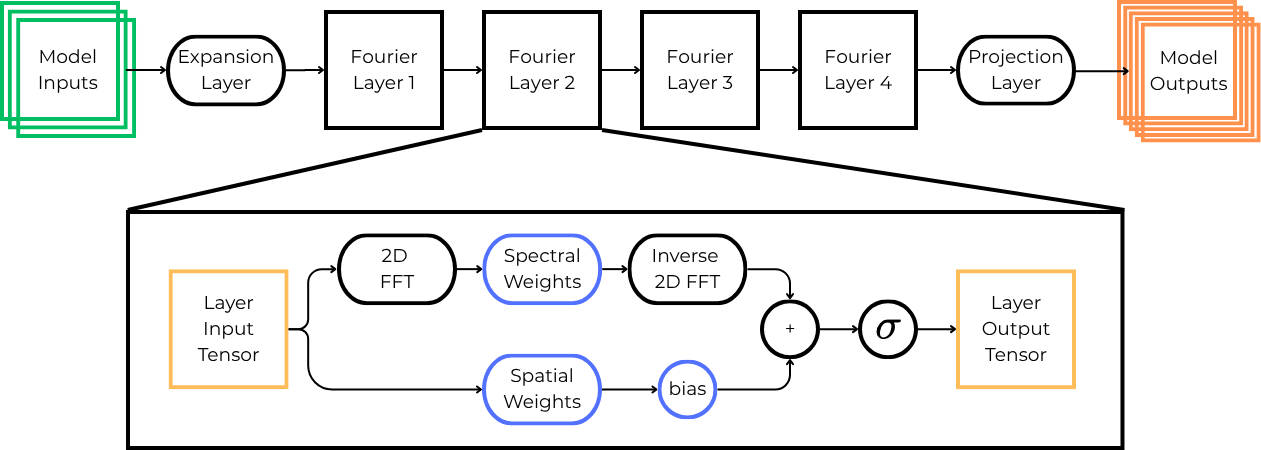
\includegraphics[width=\textwidth]{Figures/Methods/FNO_architecture.png}
\caption{The FNO model architecture used in this project. The input data is first expanded according to the hidden-channels parameter, allowing multiple latent features to be represented between Fourier layers. Each Fourier layer is shown in detail in the expanded view. The data passing through a Fourier layer is processed through two learned branches: a pointwise branch, which applies a learned linear transformation in the spatial representation, and a spectral branch, which applies a fast Fourier transform (FFT), multiplies the retained Fourier modes by learned spectral weights, and then applies an inverse FFT. The outputs of both branches, along with a learnable bias term, are summed before passing through a nonlinear activation function. After passing through four Fourier layers, the latent representation is projected from the hidden-channel dimensionality to the final output dimensions.}
\label{fig:FNO_architecture}
\end{figure}


%%%%%%%%%%%%%%%%%%%%%%%%%%%%%%%%%%%%%%%%%%%%%%%%%%%%%%%%%%%%%%%%%%%%%%
\subsection{Metamaterial Design Space}
\label{ssec:metamaterial_design_space}
To train a surrogate model capable of predicting acoustic eigenmodes, a representative design space of acoustic metamaterials must first be defined. The design space was selected to provide sufficient geometric and material complexity to demonstrate operator learning for eigenvalue PDEs while maintaining computationally tractable finite element simulations for dataset generation.

The dataset is restricted to two-dimensional acoustic metamaterials composed of infinitely repeating square unit cells exhibiting eight-fold symmetry. Each unit cell is discretized onto a $32\times32$ spatial grid and represented by three material-property channels corresponding to the normalized elastic modulus, density, and Poisson's ratio. Material properties are normalized to the interval $[0,1]$ to improve numerical conditioning during training, while the corresponding physical values are recovered using the fixed material constants listed in Table \ref{tab:parameter_ranges}. The two constituent materials were chosen to represent a stiff steel alloy and a compliant polymer.

\begin{table}[h]
  \centering
  \begin{tabular}{|c|c|c|c|c|c|c|}
    \hline
    $\text{Parameter}$ & $E_{\text{polymer}}$ & $E_{\text{steel}}$ & $\rho_{\text{polymer}}$ & $\rho_{\text{steel}}$ & $\nu_{\text{polymer}}$ & $\nu_{\text{steel}}$ \\
    \hline
    $\text{Units}$ & $\text{Pa}$ & $\text{Pa}$ & $\text{kg/m}^3$ & $\text{kg/m}^3$ & -- & -- \\
    \hline
    $\text{Value}$ & $1 \times 10^6$ & $2 \times 10^{9}$ & $1200$ & $8000$ & $0.45$ & $0.3$ \\
    \hline
  \end{tabular}
  \caption{Ranges for material parameters. The hard material is chosen to be a common steel alloy and the soft material a rubbery polymer.}
  \label{tab:parameter_ranges}
\end{table}

Unit-cell geometries are synthesized by sampling a Gaussian process with a periodic covariance kernel and subsequently enforcing eight-fold symmetry. This procedure produces smoothly varying spatial material distributions while ensuring compatibility with periodically tiled square lattices. The sampled field assumes values between $0$ and $1$, where $0$ represents pure polymer, $1$ represents pure steel, and intermediate values denote an effective mixture of the two materials below the spatial resolution of the discretization.

To investigate the influence of geometry representation on model performance, two classes of unit cells were generated. The first consists of the continuous-valued Gaussian process realizations described above and is referred to as the \emph{continuous geometry} dataset. The second is obtained by thresholding the Gaussian process samples to binary numbers, producing geometries composed exclusively of polymer and steel. This second collection is referred to as the \emph{discrete geometry} dataset. Each representation comprises approximately one-half of the total dataset.

\begin{figure}[H]
  \centering
  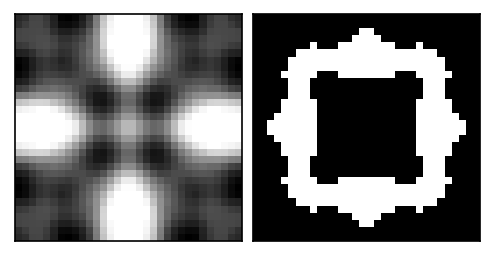
\includegraphics[width=0.5\textwidth]{Figures/Methods/continuous_and_binary_geometry_example.png}
  \caption{Example of a continuous geometry (left) and a discrete geometry (right) generated using the above process and parameters.}
  \label{fig:example_geometries}
\end{figure}

%%%%%%%%%%%%%%%%%%%%%%%%%%%%%%%%%%%%%%%%%%%%%%%%%%%%%%%%%%%%%%%%%%%%%%
\subsection{Wave Propagation Simulations} 
\label{ssec:wave_propagration_simulations}

For each metamaterial geometry, wave propagation is simulated by solving the frequency-domain linear elastodynamic equation with finite element analysis (FEA). After spatial discretization and enforcement of Bloch periodicity, the governing problem takes the generalized eigenvalue form
\begin{equation}
\label{eqn:eig_PDE}
\left( \mathbf{K}_r(\mathbf{k}) - \omega^2 \mathbf{M}_r(\mathbf{k}) \right) \mathbf{u} = \mathbf{0},
\end{equation}
where $\omega$ is the angular eigenfrequency, $\mathbf{u}$ is the corresponding complex Bloch displacement eigenvector, and $\mathbf{k}$ is the wavevector in the irreducible Brillouin zone (IBZ). The reduced stiffness and mass matrices $\mathbf{K}_r(\mathbf{k})$ and $\mathbf{M}_r(\mathbf{k})$ are obtained from geometry-dependent global finite-element matrices $\mathbf{K}$ and $\mathbf{M}$ via a wavevector-dependent Bloch transformation matrix $\mathbf{T}(\mathbf{k})$,
\begin{equation}
\label{eqn:reduced_KM}
\mathbf{K}_r(\mathbf{k}) = \mathbf{T}(\mathbf{k})^{\dagger}\mathbf{K}\,\mathbf{T}(\mathbf{k}),
\qquad
\mathbf{M}_r(\mathbf{k}) = \mathbf{T}(\mathbf{k})^{\dagger}\mathbf{M}\,\mathbf{T}(\mathbf{k}),
\end{equation}
with $(\cdot)^{\dagger}$ the Hermitian transpose. Here $\mathbf{T}(\mathbf{k})$ maps the full mesh degrees of freedom to an independent set while applying phase factors $\mathrm{e}^{i\mathbf{k}\cdot\mathbf{R}}$ across periodic faces of the unit cell; $\mathbf{K}$ and $\mathbf{M}$ themselves depend only on the material field and are assembled once per geometry. These intermediate matrices are described briefly so the reader can compare the explicit FEA pipeline (Figure~\ref{fig:FEA_full_process}) with the Fourier neural operator architecture in Section~\ref{ssec:fourier_neural_operator}; they are not inputs to the neural operator.

The IBZ is discretized into $25$ $x$ wave numbers and $13$ $y$ wave numbers, totaling $25 \times 13 = 325$ unique wavevectors covering the IBZ half plane. For each wavevector, the six lowest eigenfrequencies (bands) were computed using a custom FEA MATLAB script (see Section~\ref{sec:Repository} for implementation details). 

Each eigenvector $\mathbf{u}$ consists of two complex-valued displacement fields, $(u_x,u_y)$, which are separated into their real and imaginary components to produce four real-valued output channels, $(u_{x,real},u_{x,imag},u_{y,real},u_{y,imag})$. The corresponding eigenfrequency $\omega$ is encoded as a spatially uniform fifth channel, resulting in a target tensor of size $5\times32\times32$. Combined with the three-channel material representation described in the previous subsection, each simulation therefore produces a supervised learning sample mapping
\begin{equation*}
\mathbb{R}^{3\times32\times32}
\rightarrow
\mathbb{R}^{5\times32\times32}.
\end{equation*}
The overall finite element data-generation procedure is summarized in Figure \ref{fig:FEA_full_process}.

\begin{figure}[H]
  \centering
  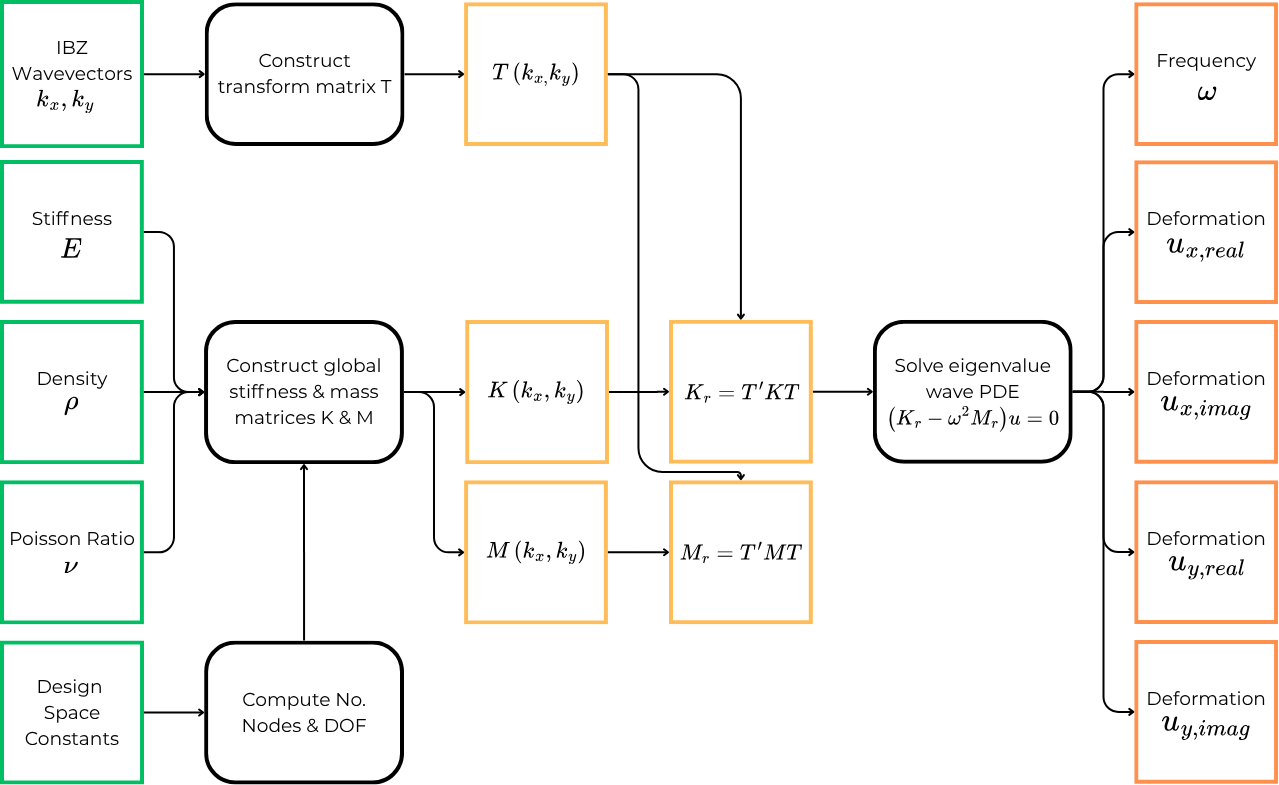
\includegraphics[width=\textwidth]{Figures/Methods/distilled_FEA_process.png}
  \caption{Flowchart of the FEA data generation method. Green squares represent varying inputs to the process, and orange squares represent computed quantities of the FEA process. Black rounded rectangles represent subroutines of the FEA process. The process starts with inputs of defined densities, stiffnesses, and Poisson ratios for each pixel of a metamaterial unit cell geometry (each a $32 \times 32$ pixel grid of values ranging from 0 to 1), along with a chosen $k_x$ and $k_y$ wavevector representing the stimulus to the metamaterial. A custom optimized FEA solver takes these inputs and produces intermediate matrices $(\mathbf{K},\mathbf{M},\mathbf{T})$, forms the reduced operators $(\mathbf{K}_r,\mathbf{M}_r)$, and then solves Eq.~\eqref{eqn:eig_PDE} for the displacement fields (eigenvectors) and frequencies $\omega$ (eigenvalues) for the given inputs.}
  \label{fig:FEA_full_process}
\end{figure}

%%%%%%%%%%%%%%%%%%%%%%%%%%%%%%%%%%%%%%%%%%%%%%%%%%%%%%%%%%%%%%%%%%%%%%
\subsection{Input Wavelet Encoding}
\label{ssec:input_wavelet_encoding}
To allow the FNO model to toggle between PDE solutions for a given geometry, information must be fed to the model indicating which excitation waveform (wavevectors) and deformation mode (band) we are looking for a solution to. This information is given in the form of a wavevector embedding, which we have found to yield superior results compared with a constant field embedding (2D matrices of the same value) or a sinusoidal embedding (2D sinusoidal fields with constants encoded as the sinusoidal frequency). A discussion on why wavelet encodings are superior is found in Section~\ref{ssec:band_wavevector_encoding}.

For the wavelet encodings, we use a 1D Gabor wavelet transform to map band numbers to unique wavelet images (see Algorithm \ref{alg:1d_gabor_embedding}), and a 2D Gabor wavelet transform to map x and y wavevectors to another set of unique wavelet images (see Algorithm \ref{alg:2d_gabor_embedding}). These representations show rich variation both in the spatial domain and in the Fourier domain, which allows for FNO model weights of both branches to richly interact with the wavelet representation, leading to better learning outcomes. 

\begin{figure}[H]
    \centering
    \begin{subfigure}{\textwidth}
        \centering
        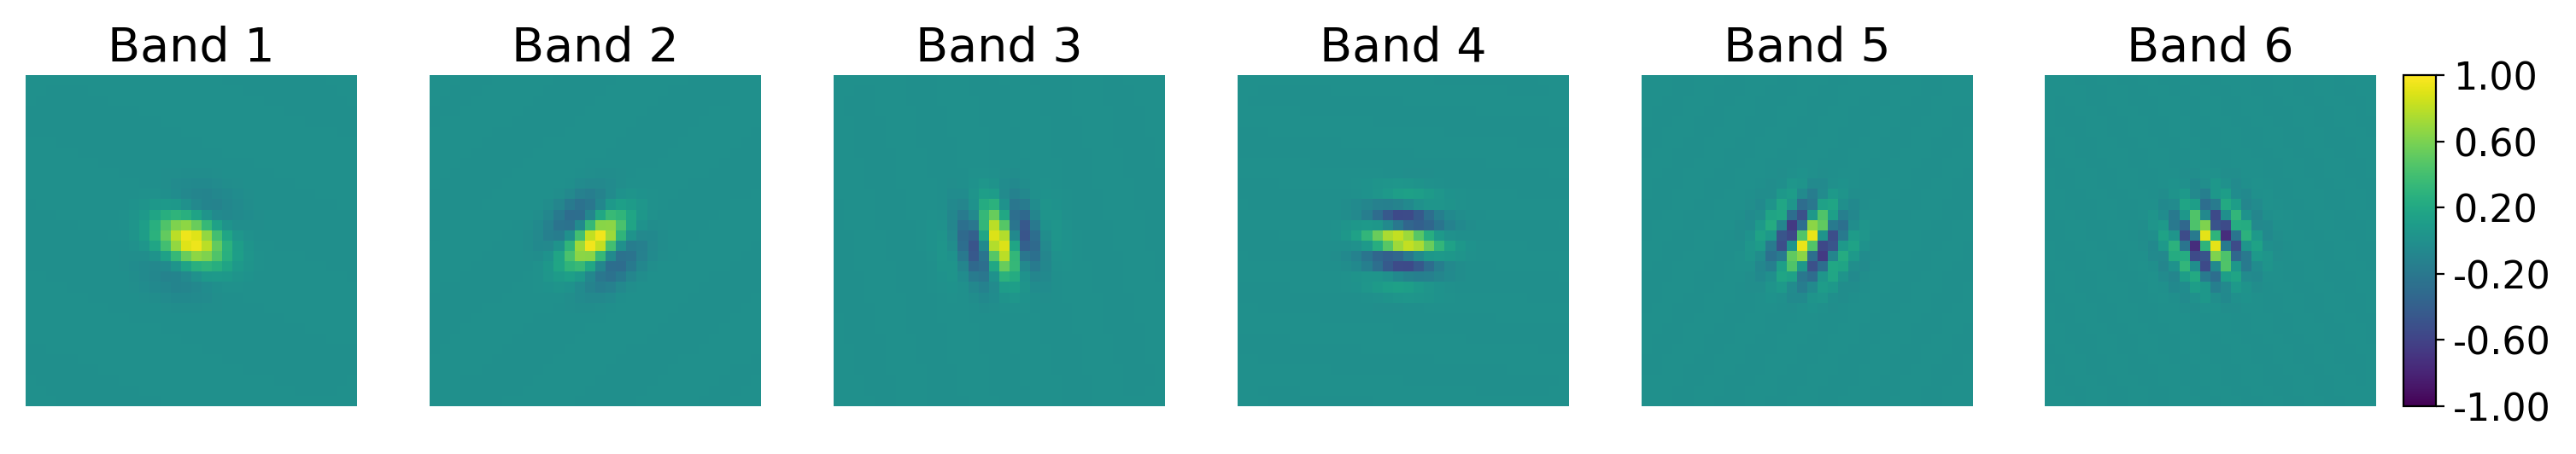
\includegraphics[width=\textwidth]{Figures/Methods/1D wavelet encoding.png}
        \caption{The wavelet spatial encoding for band integer.}
        \label{fig:1D_wavelet_encoding_spatial}
    \end{subfigure}  
    \begin{subfigure}{\textwidth}
        \centering
        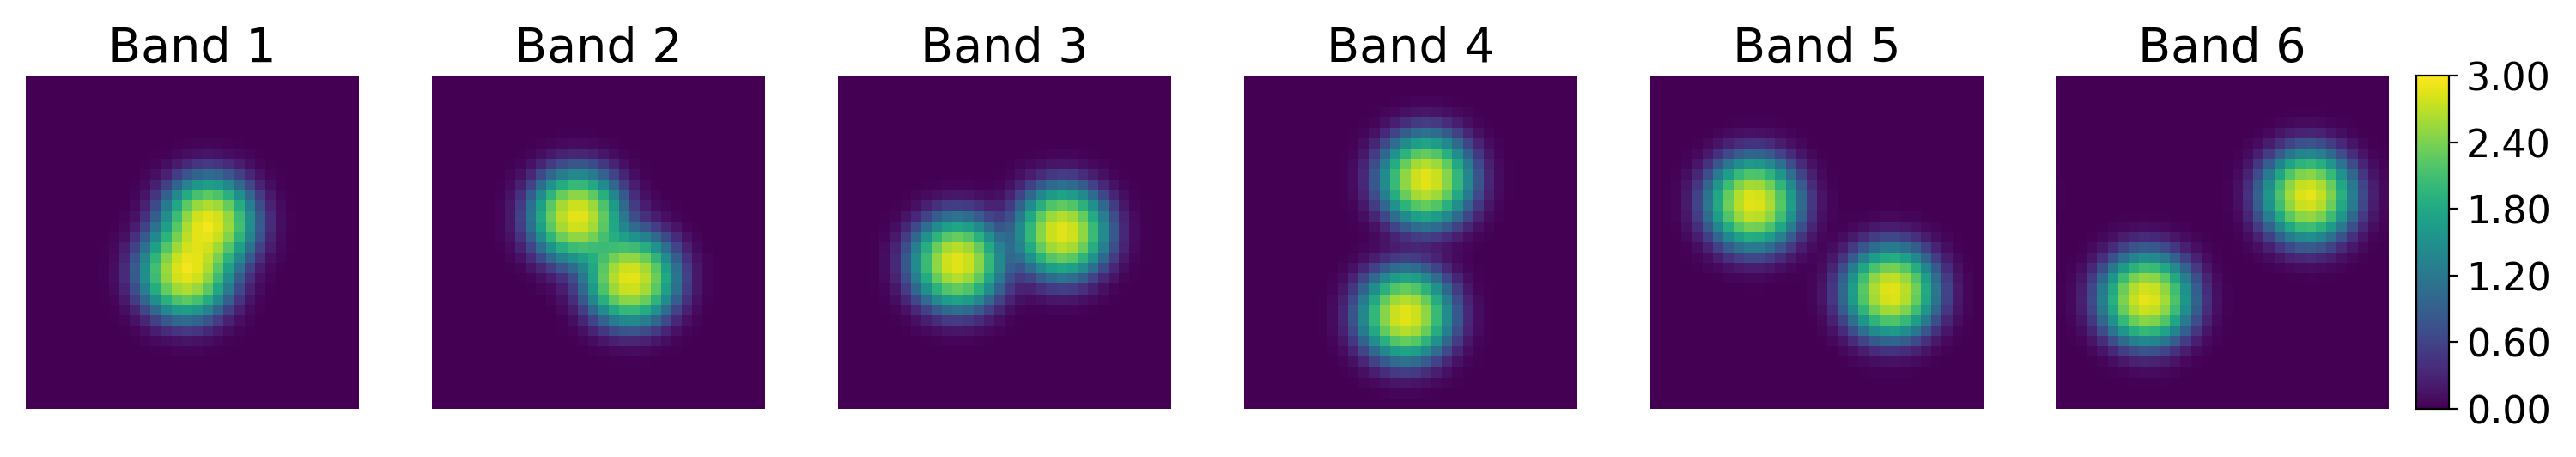
\includegraphics[width=\textwidth]{Figures/Methods/1D wavelet encoding fft.png}
        \caption{The FFT of the above wavelet spatial encodings.}
        \label{fig:1D_wavelet_encoding_fft}
    \end{subfigure}
    \caption{The wavelet encoding of the band integer (fig. \ref{fig:1D_wavelet_encoding_spatial}) and its FFT (fig. \ref{fig:1D_wavelet_encoding_fft}). Each band corresponds to a unique wavelet with representation in both spatial and spectral domains.}
    \label{fig:1D_wavelet_encoding}
\end{figure}

\begin{figure}[H]
    \centering
    \begin{subfigure}{\textwidth}
        \centering
        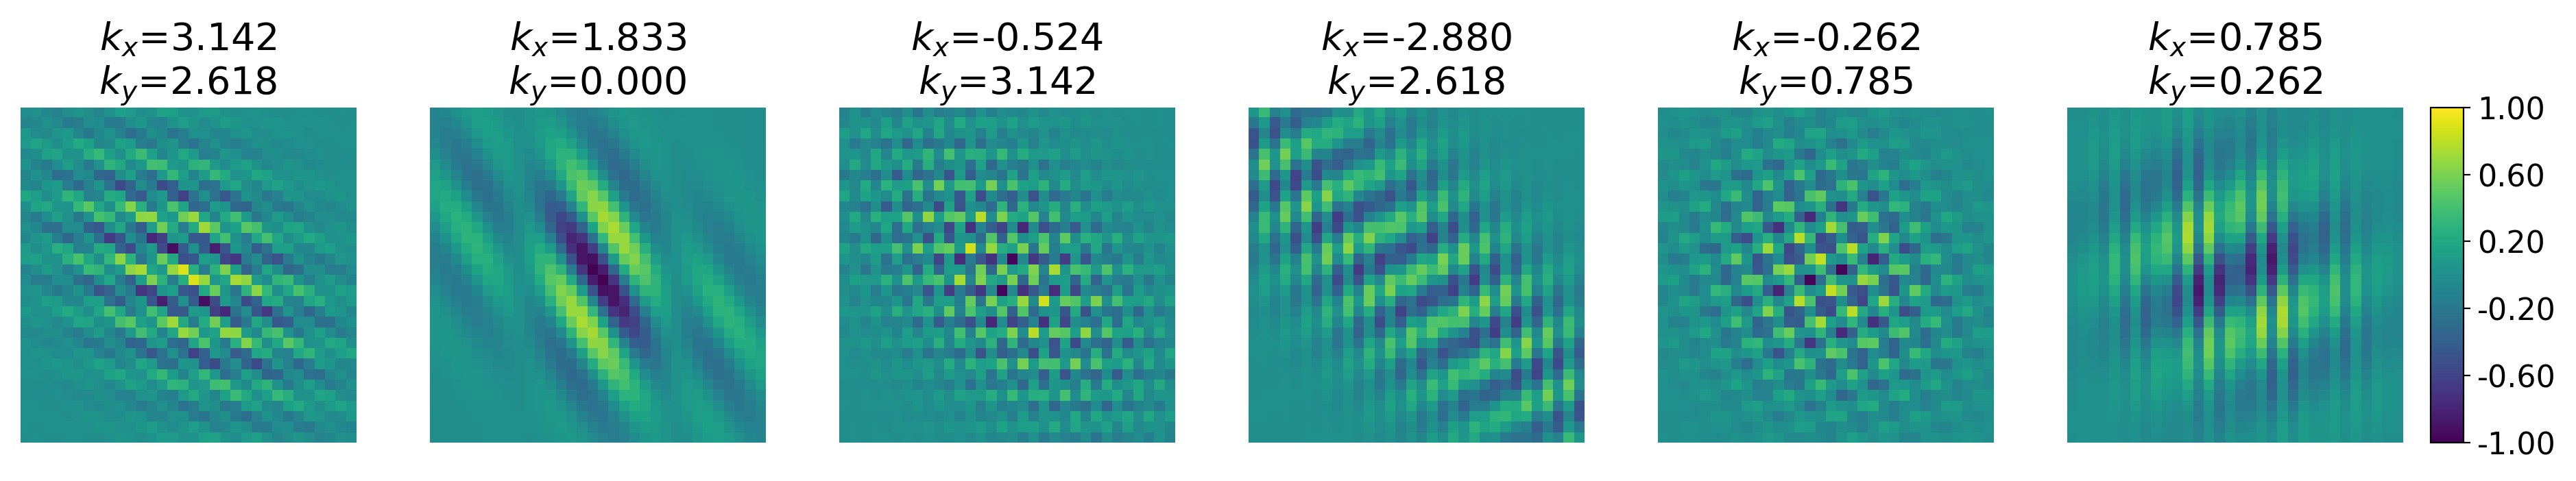
\includegraphics[width=\textwidth]{Figures/Methods/2D wavelet encoding.png}
        \caption{The wavelet spatial encoding for $x$ and $y$ wavevectors.}
        \label{fig:2D_wavelet_encoding_spatial}
    \end{subfigure}  
    \begin{subfigure}{\textwidth}
        \centering
        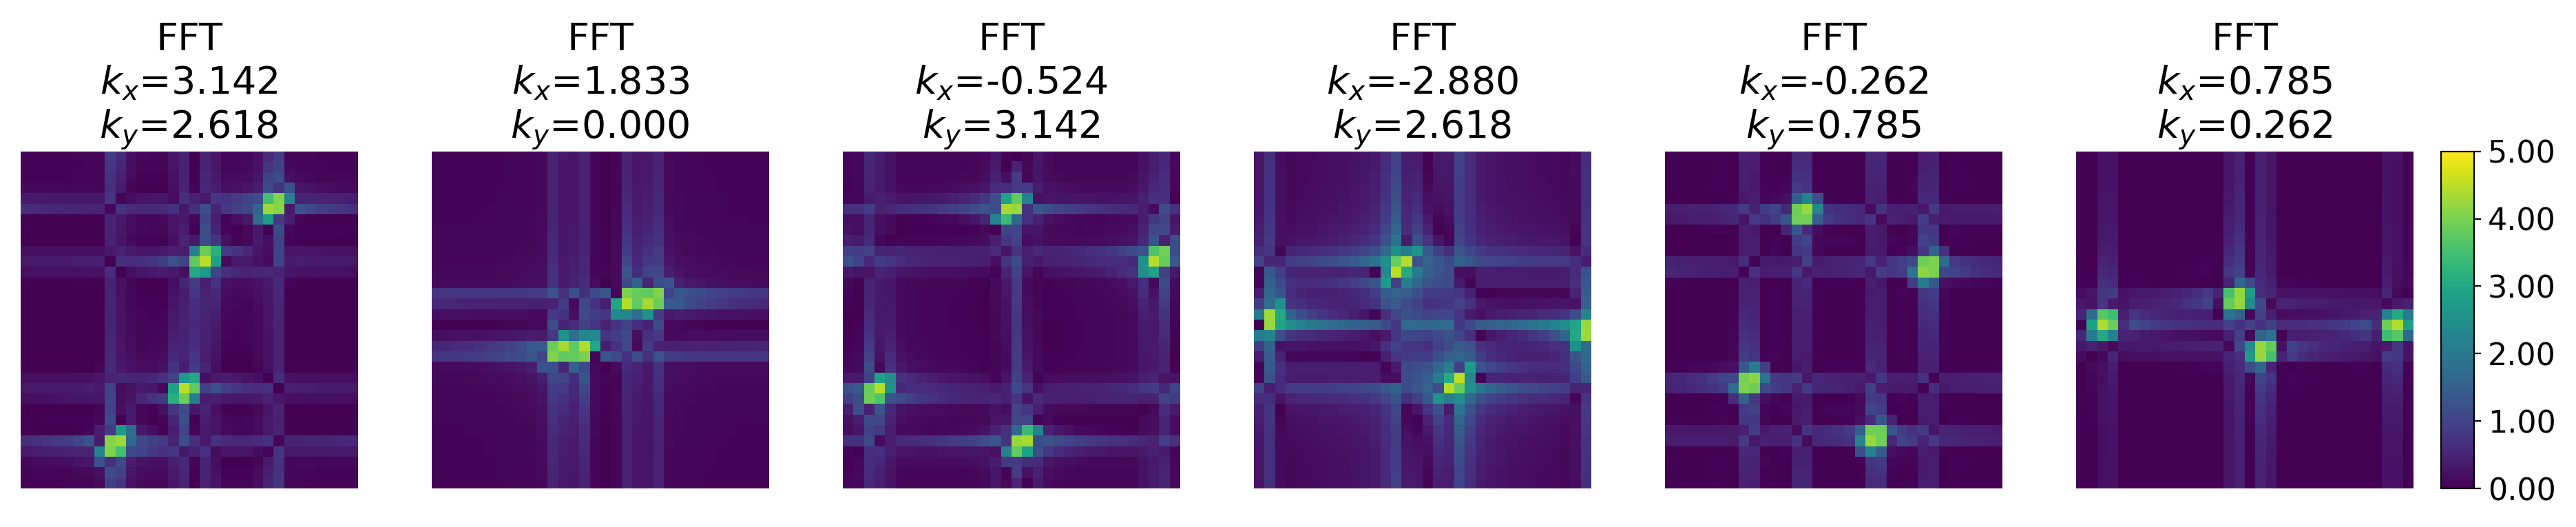
\includegraphics[width=\textwidth]{Figures/Methods/2D wavelet encoding fft.png}
        \caption{The FFT of the above wavelet spatial encodings.}
        \label{fig:2D_wavelet_encoding_fft}
    \end{subfigure}
    \caption{The wavelet encoding of the $x$ and $y$ wavevectors (\ref{fig:2D_wavelet_encoding_spatial}) and its FFT \ref{fig:2D_wavelet_encoding_fft}. The actual wavevectors are shown in the subplot titles. For each $k_x$ and $k_y$ value pair, there is a unique mapping in both the spatial and spectral domain representations.}
    \label{fig:2D_wavelet_encoding}
\end{figure}

When encoding continuous constants with oscillatory functions on a finite grid, it is important to verify that distinct parameter values do not alias into nearly identical patches. Otherwise the model cannot distinguish neighboring wavevectors, and mode selection collapses. We therefore checked pairwise cosine similarity of the mean-centered $\log_{10}|\mathrm{FFT}|$ spectra of all $325$ IBZ wavevector encodings produced by Algorithm~\ref{alg:2d_gabor_embedding} (Supplementary Information). The resulting similarity matrix is shown in Figure~\ref{fig:wavevector_encoding_similarity}; the maximum off-diagonal similarity is $0.862$, well below near-duplicate levels, confirming that the chosen encoding constants introduce no appreciable aliasing across the IBZ grid.

\begin{figure}[H]
  \centering
  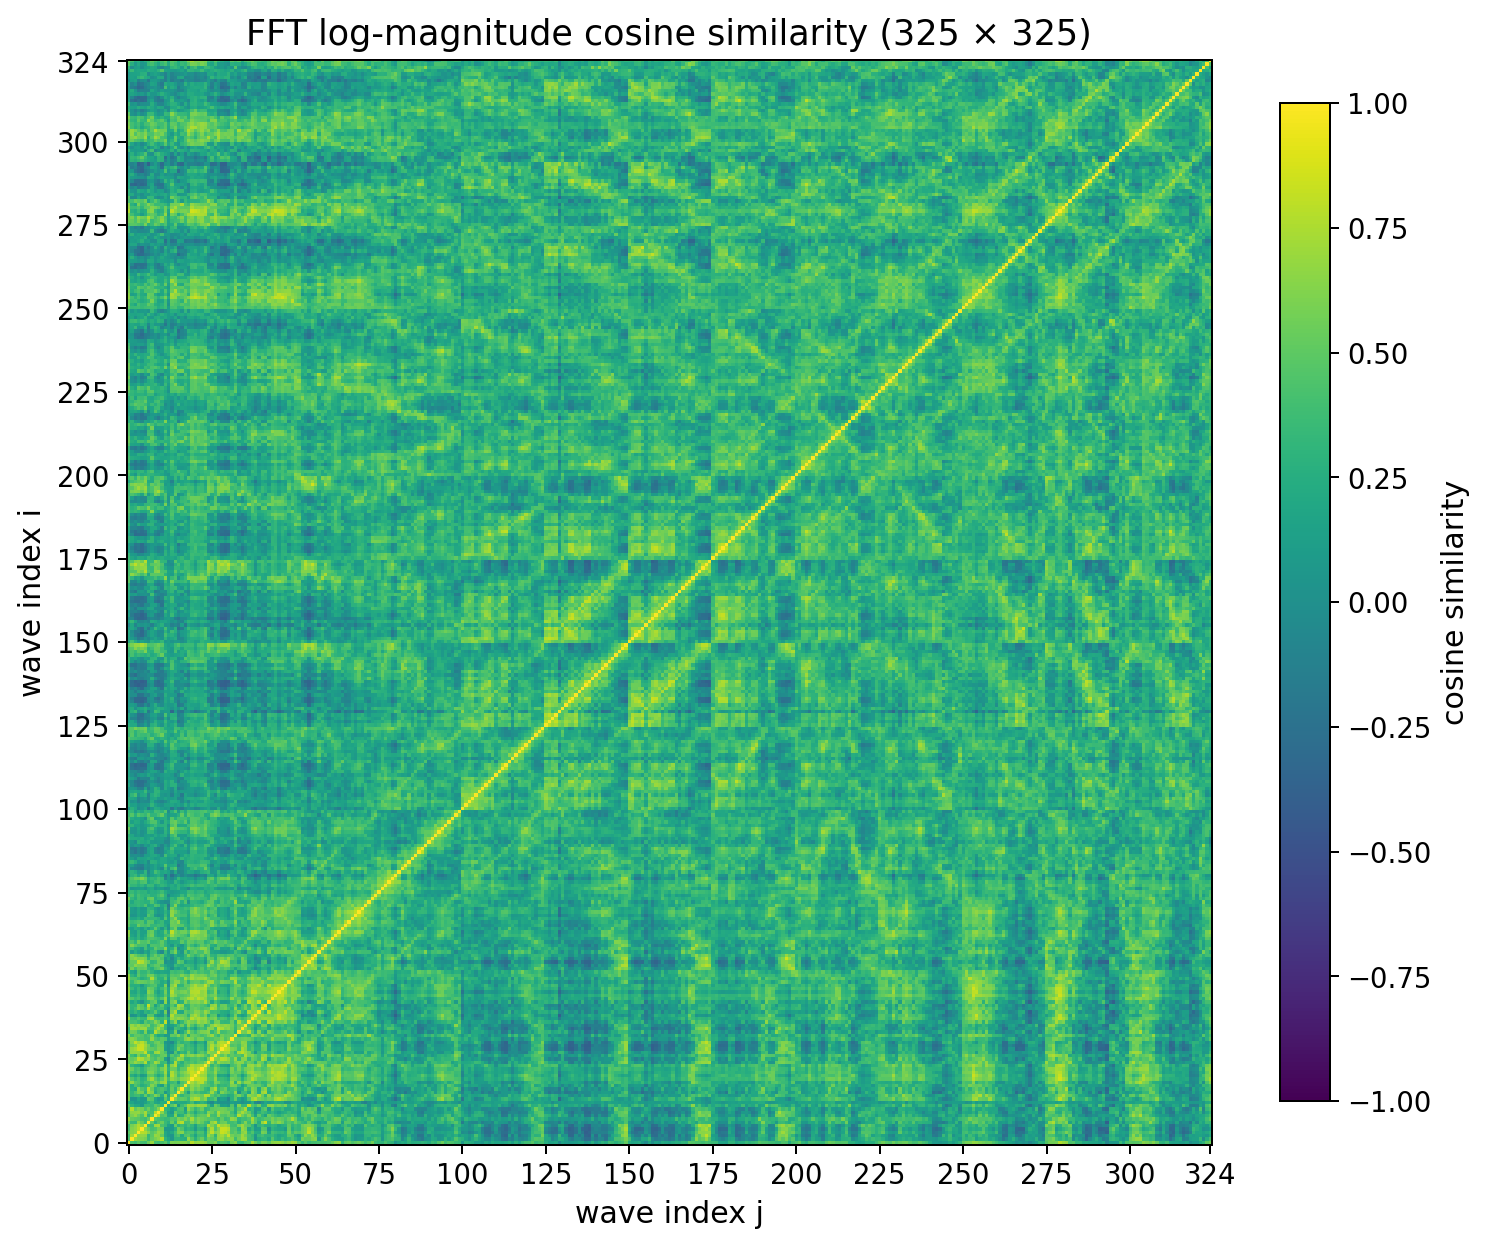
\includegraphics[width=0.75\textwidth]{Figures/Methods/fft_log_cosine_similarity_heatmap_fscale41_offset2p2_sigma0p5_kx13_ky25.png}
  \caption{Pairwise cosine similarity of mean-centered $\log_{10}|\mathrm{FFT}|$ spectra for the $325$ IBZ wavevector encodings generated by Algorithm~\ref{alg:2d_gabor_embedding}. The maximum off-diagonal similarity is $0.862$, indicating that distinct $(k_x,k_y)$ pairs remain spectrally separable on the $32\times32$ grid.}
  \label{fig:wavevector_encoding_similarity}
\end{figure}

%%%%%%%%%%%%%%%%%%%%%%%%%%%%%%%%%%%%%%%%%%%%%%%%%%%%%%%%%%%%%%%%%%%%%%


%%%%%%%%%%%%%%%%%%%%%%%%%%%%%%%%%%%%%%%%%%%%%%%%%%%%%%%%%%%%%%%%%%%%%%
\subsection{Dataset Construction} 
\label{ssec:dataset_construction}
Our full dataset contains 24000 geometries, randomly generated as described in prior subsections. Half are discrete valued with only 0s or 1s in each pixel location representing one of the two materials, while the other half are continuous valued with any value between 0 and 1 inclusive at each pixel location, representing blended materials at each pixel location. Each geometry has 6 possible bands each with 325 possible wavevectors (representing a mesh grid the IBZ half plane) per band, resulting in $24000 \times 6 \times 325 = 46,800,000$ sample pairs of inputs with shape $(3 \times 32 \times 32)$ and outputs of shape $(5 \times 32 \times 32)$. The data is stored with float16 datatype format in PyTorch tensors. 

% Due to computational and memory constraints, for each of the 9600 geometries, a random 1/4 of the 325 waveforms and 1/2 of the 6 deformation modes (i.e., 3 bands) were retained for FNO training. This stochastic downsampling maintains a diverse sampling of wave-structure interactions while reducing the size of the training dataset by a factor of 8.

\begin{figure}[H]
  \centering
  \begin{subfigure}[c]{0.5\textwidth}
    \centering
    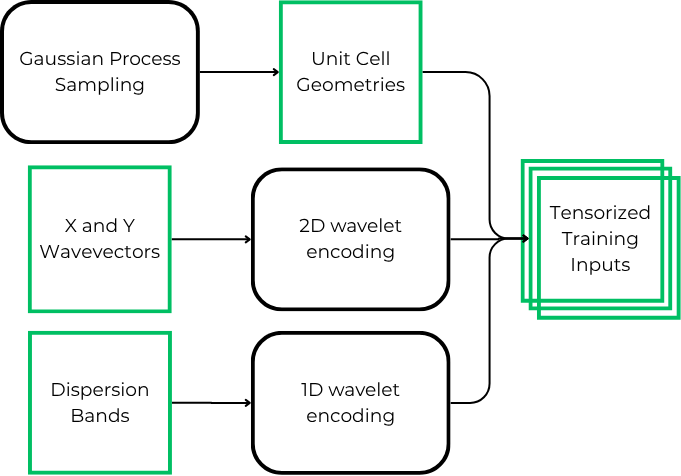
\includegraphics[scale=0.35]{Figures/Methods/distilled_input_tensorization.png}
    %
\includegraphics{Figures/distilled_input_tensorization.png}
    \caption{Construction of the input tensors}
    \label{fig:input_dataset_construction}
  \end{subfigure}%
  \hfill
  \begin{subfigure}[c]{0.5\textwidth}
    \centering
    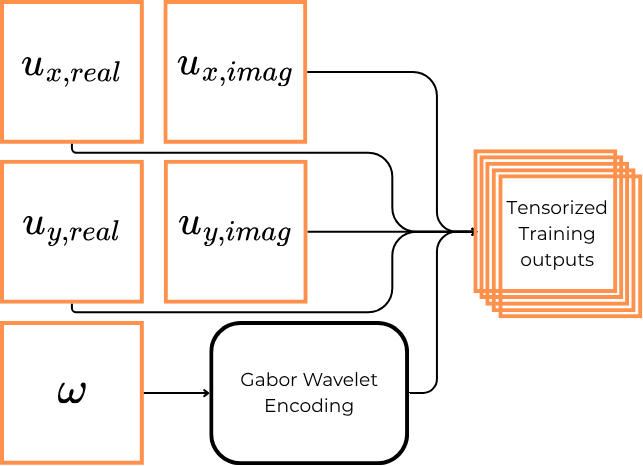
\includegraphics[scale=0.35]{Figures/Methods/distilled_output_tensorization2.png}
    %
\includegraphics{Figures/distilled_outout_tensorization.png}
    \caption{Construction of the output tensors}
    \label{fig:output_dataset_construction}
  \end{subfigure}
  \caption{Subfigure \subref{fig:input_dataset_construction} and \subref{fig:output_dataset_construction} shows the process of input data from subsection \ref{ssec:metamaterial_design_space} and output data from subsection \ref{ssec:wave_propagration_simulations} being tensorized for ingestion to the FNO model respectively. Note the wavelet embedding steps on fundamentally scalar quantities.}
  \label{fig:dataset_construction}
\end{figure}

%%%%%%%%%%%%%%%%%%%%%%%%%%%%%%%%%%%%%%%%%%%%%%%%%%%%%%%%%%%%%%%%%%%%%%


\subsection{Training Procedure}
\label{ssec:training_procedure}
The Fourier Neural Operator was trained using supervised learning on paired inputs and outputs described in Section \ref{sec:Methodology}. Each training sample consists of a $3 \times 32 \times 32$ input tensor (geometry and wavelet embeddings) and a $5 \times 32 \times 32$ output tensor (displacement field components and eigenfrequency).

6 loss functions were trialed as performance evaluation criterion: mean absolute error (MAE), mean squared error (MSE), normalized MAE, normalized MSE, Huber (smooth L1), and structural similarity index (SSI). Losses were evaluated and aggregated across all 5 output channels. The best performing loss criterion is the Huber loss and is shown below. Details on the other loss functions trialed can be found in Supplemental Information.
% \begin{equation*}
%     \mathcal{L}_{\text{MAE}} = \frac{1}{HW} \sum_{i=0}^{H-1} \sum_{j=0}^{W-1} \sum_{c=0}^{4} \left| \hat{u}_{c}(i,j) - u_{c}(i,j) \right|
% \end{equation*}

% \begin{equation*}
%     \mathcal{L}_{\text{MSE}} = \frac{1}{HW} \sum_{i=0}^{H-1} \sum_{j=0}^{W-1} \sum_{c=0}^{4} \left( \hat{u}_{c}(i,j) - u_{c}(i,j) \right)^2
% \end{equation*}
% \begin{equation*}
%     \mathcal{L}_{\text{NMAE}} = \frac{1}{HW} \sum_{i=0}^{H-1} \sum_{j=0}^{W-1} \sum_{c=0}^{4} \frac{\displaystyle \left| \hat{u}_{c}(i,j) - u_{c}(i,j) \right|}{\left| u_{c}(i,j) \right| + \varepsilon}
% \end{equation*}
% \begin{equation*}
%     \mathcal{L}_{\text{NMSE}} = \frac{1}{HW} \sum_{i=0}^{H-1} \sum_{j=0}^{W-1} \sum_{c=0}^{4} \frac{\displaystyle \left(\hat{u}_{c}(i,j) - u_{c}(i,j) \right)^2}{\left( u_{c}(i,j) \right)^2 + \varepsilon}
% \end{equation*}
% \begin{equation*}
% \mathcal{L}_{\text{Huber}} = 
% \begin{cases}
% \mathcal{L}_{\text{MAE}}, & \mathcal{L}_{\text{Huber}} \ge 10^{-3}, \\
% \mathcal{L}_{\text{MSE}}, & \mathcal{L}_{\text{Huber}} < 10^{-3}.
% \end{cases}
% \end{equation*}

\begin{equation*}
\mathcal{L}_{\text{Huber}}
=
\frac{1}{HW}
\sum_{i=0}^{H-1}
\sum_{j=0}^{W-1}
\sum_{c=0}^{4}
\begin{cases}
\dfrac{1}{2}\left(\hat{u}_c(i,j)-u_c(i,j)\right)^2,
&
\left|\hat{u}_c(i,j)-u_c(i,j)\right|\le\delta,
\\[2ex]
\delta\left(
\left|\hat{u}_c(i,j)-u_c(i,j)\right|
-\dfrac{\delta}{2}
\right),
&
\left|\hat{u}_c(i,j)-u_c(i,j)\right|>\delta.
\end{cases}
\end{equation*}

% \begin{equation*}
% \mathcal{L}_{\text{SSIM}}
% =
% 1
% -
% \frac{1}{5}
% \sum_{c=0}^{4}
% \frac{
% \left(2\mu_{u_c}\mu_{\hat{u}_c}+C_1\right)
% \left(2\sigma_{u_c\hat{u}_c}+C_2\right)
% }{
% \left(\mu_{u_c}^2+\mu_{\hat{u}_c}^2+C_1\right)
% \left(\sigma_{u_c}^2+\sigma_{\hat{u}_c}^2+C_2\right) 
% }, \quad \text{where}
% \end{equation*}
% \begin{equation*}
% \mu_{u_c}
% =
% \frac{1}{HW}
% \sum_{i=0}^{H-1}
% \sum_{j=0}^{W-1}
% u_c(i,j), \quad 
% \sigma_{u_c\hat{u}_c}
% =
% \frac{1}{HW}
% \sum_{i=0}^{H-1}
% \sum_{j=0}^{W-1}
% \left(u_c(i,j)-\mu_{u_c}\right)
% \left(\hat{u}_c(i,j)-\mu_{\hat{u}_c}\right)
% \end{equation*}

where $H = W = 32$ (pixels) and $c \in \{0,1,2,3,4\}$ corresponds to the 5 output channels: eigenfrequency, followed by real and imaginary components of x and y displacements.

For training the FNO model, combinations of model layers, hidden channels, activation function, loss function, optimizer, and training hyperparameters were trialed. The ADAMW optimizer was found to achieve the best performance compared with other flavors of momentum based optimizers and SGD. The model and training hyperparameters tuned are showed in table \ref{tab:training_hyperparameters} in \ref{sec:supplement}, with the best performing combination italicized.

% Training was performed on a randomly down-selected subset of the full dataset. Each of the 9600 geometries was paired 81 waveforms (randomly sampled from the full 325) and 3 dispersion bands (randomly sampled from the full 6), resulting in reduced memory overhead and faster training convergence while maintaining diversity across samples.



The best combination for model hyperparameters was found to be 4 Fourier layers, 128 hidden channels, and GELU nonlinear activation function. At this layer count and hidden channel count, performance was asymptotic and greater amounts of either would drive the model further into the overfit region as well as add on additional training time. The best combination for trianing hyperparameters were the Huber loss, which is to use a which would was found to be 12 epochs, Different hyperparameters of FNO model tried in combinations. 4 Fourier layers, with 64 hidden channels and GELU activation function were found to be where performance started to asymptote with increasing model complexity, and so it was not worth the computational costs in training to use more layers or hidden channels. These are the final combination of model hyperparameters from which all data presented in this article is generated.

% \begin{figure}[H]
%     \centering
%     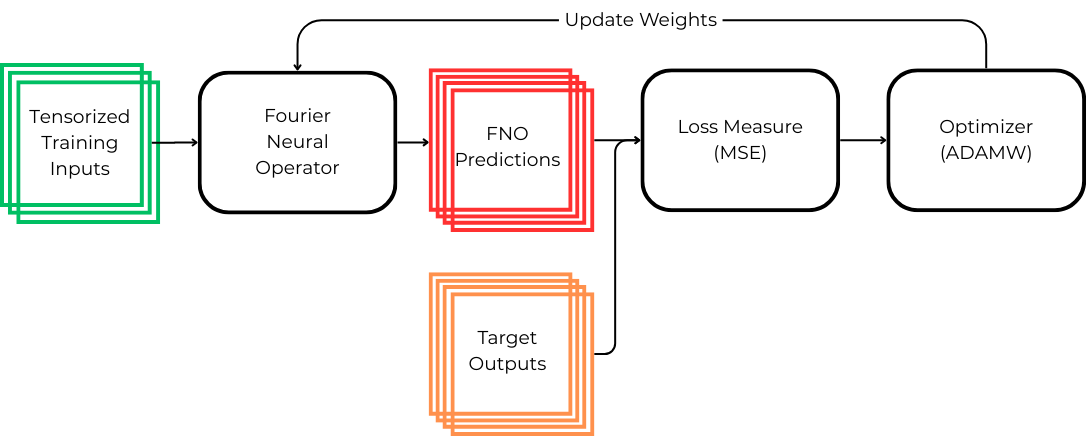
\includegraphics[scale=0.5]{Figures/Methods/model_training.png}
%     \caption{Schematic of model training loop. For compute speed and efficiency, batches of 256 inputs and outputs are run in parallel each loop.}
%     \label{fig:model_training}
% \end{figure}
% While L2 loss was used for training due to its commonality and prior successes in imaged based machine learning tasks, we chose to use L1 as the evaluation criterion for ease of interpretability of how off the model is on average for pixel predictions. Schematics of the usage of the two loss criterion in training and evaluation are shown in figure \ref{}
% \begin{figure}[H]
%     \centering
%     \begin{subfigure}[c]{0.8\textwidth}
%         \centering
%         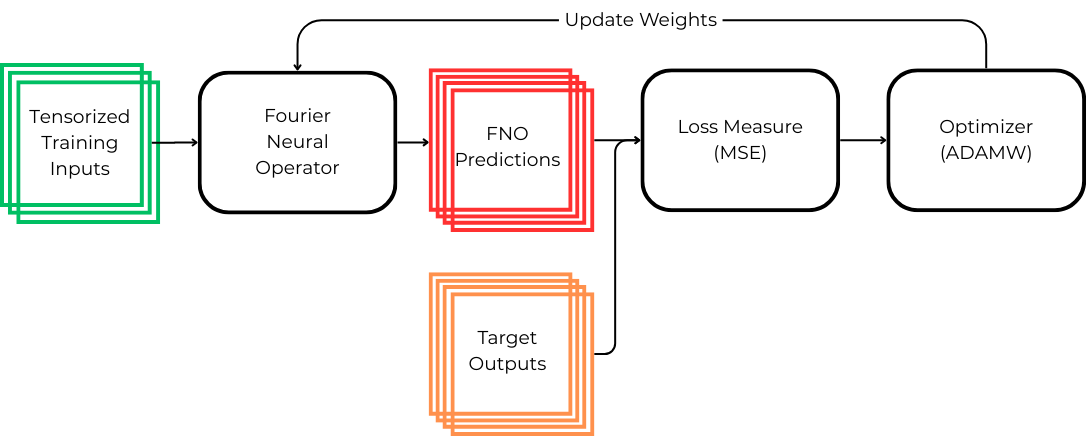
\includegraphics[scale=0.5]{Figures/Methods/model_training.png}
%         \caption{Schematic of model training loop. For compute speed and efficiency, batches of 256 inputs and outputs are run in parallel each loop.}
%         \label{fig:model_training}
%     \end{subfigure}%
%     \vspace{1em}
%     \begin{subfigure}[c]{0.8\textwidth}
%     \centering
%         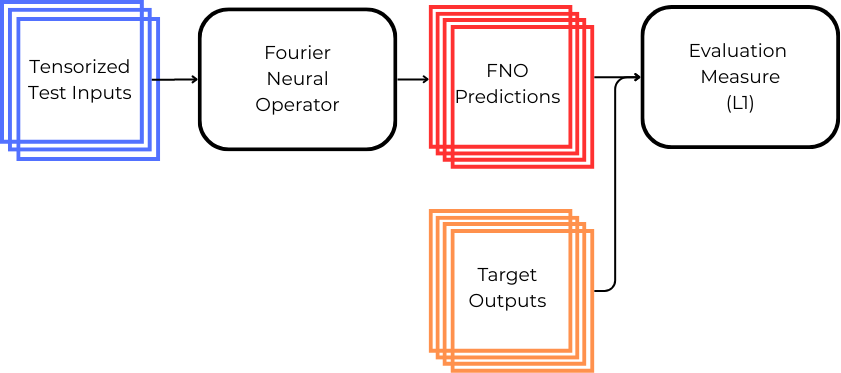
\includegraphics[scale=0.5]{Figures/Methods/model_evaluation.png}
%         \caption{Schematic of the model evaluation process. Absolute error is used here to have a simple interpretation of performance. The test datasets are of previously unseen geometries, meaning the model must be able to generalize from the highly limited number of possible geometries it is shown to the whole design space of possible geometries to do well in evaluations.}
%         \label{fig:model_evaluation}
%     \end{subfigure}
%     \caption{Subfigure \subref{fig:input_dataset_construction} and \subref{fig:output_dataset_construction} shows the training and evaluation process for the FNO model respectively.}
%     \label{fig:training_and_evaluation}
% \end{figure}

It was found that final model performance did not appreciably change for changes in step size or batch size fairly early on, so those two parameters were left fixed at 4 and 256 respectively for the remainder of the training runs. Learning rate and epochs to convergence as expected, had an inverse correlation. The higher the learning rate, the faster convergence happened, but there are two problems with high learning rates. The first is that the model may arrive at a more suboptimal combination of weights if the training rate is too high, because the movements in weight space during each backward pass remain too large to arrive close in weight space to where the loss minima would occur. The second, more interesting phenomena, is that if the learning rate is set higher than $\approx 10^{-2}$, there is instability introduced in the training, whereby at certain epochs, the loss would spike, and never come back down, usually plateauing, in all later epochs. This sort of spike is documented in other applications of ADAM family optimizers indicating the model is pushed into a region of weight space where the loss was flat for movements in any direction.

%%%%%%%%%%%%%%%%%%%%%%%%%%%%%%%%%%%%%%%%%%%%%%%%%%%%%%%%%%%%%%%%%%%%%%
\section{Results and Discussion}
% This section presents the final model results in the following cases:
% \begin{itemize}
%     \item[\checked] Performance on displacement field prediction
%     \item[\checked] Performance on eigenvalue prediction
%     \item[\checked] Performance across multiple geometries
%     \item[\checked] Performance variation with binary geometry discontinuity measures
%     \item[\checked] Performance variation with encoding strategies
%     \item[\unchecked] Performance variation with training hyperparameters and loss function
% \end{itemize}

% In our search through the best encoding scheme for inputs, datatype representation for outputs, model architecture hyperparameters, and training hyperparameters for our FNO eigenvalue PDE solver, we discovered the following notable results.  

%%%%%%%%%%%%%%%%%%%%%%%%%%%%%%%%%%%%%%%%%%%%%%%%%%%%%%%%%%%%%%%%%%%%%%
\subsection{Displacement Field Prediction}
We next evaluate the trained Fourier Neural Operator on its predictions of the Bloch displacement fields $(u_x,u_y)$. For each unseen test sample, the prediction error is measured by the normalized mean absolute error (NMAE) over the four real-valued displacement channels, $(u_{x,\mathrm{real}},u_{x,\mathrm{imag}},u_{y,\mathrm{real}},u_{y,\mathrm{imag}})$. Ranking samples by this NMAE defines a performance distribution from which we select representative cases at the $25$th, $50$th, and $75$th percentiles, corresponding to relatively weak, median, and relatively strong predictions. The same percentile comparison is shown for both the binarized and continuous material datasets, allowing direct visual assessment of how well the model recovers the spatial structure of the displacement modes across contrasting geometry regimes.

\subsubsection{Continuous Geometries}
\begin{figure}[H]
    \centering
    \begin{subfigure}[c]{0.75\textwidth}
        \centering
        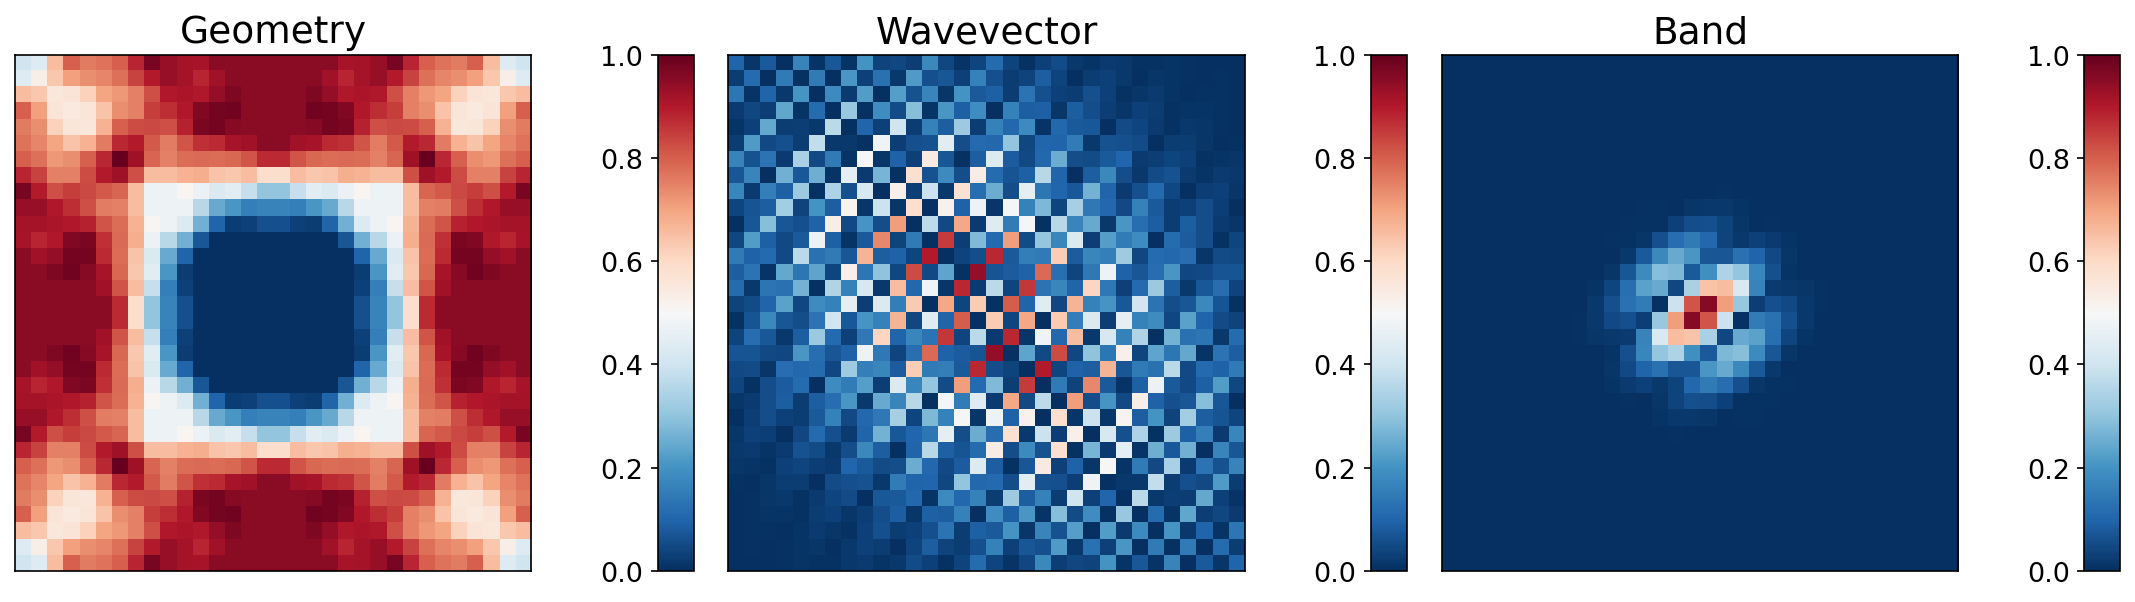
\includegraphics[width=\textwidth]{Figures/Fields C/c_test_nmae_p25_g452_w224_b1_input.png}
        \caption{Input sample at the 25th percentile of performance for unseen continuous valued geometries.}
        \label{fig:c_p25_input}
    \end{subfigure}
    \vspace{1em}
    \begin{subfigure}[c]{\textwidth}
    \centering
        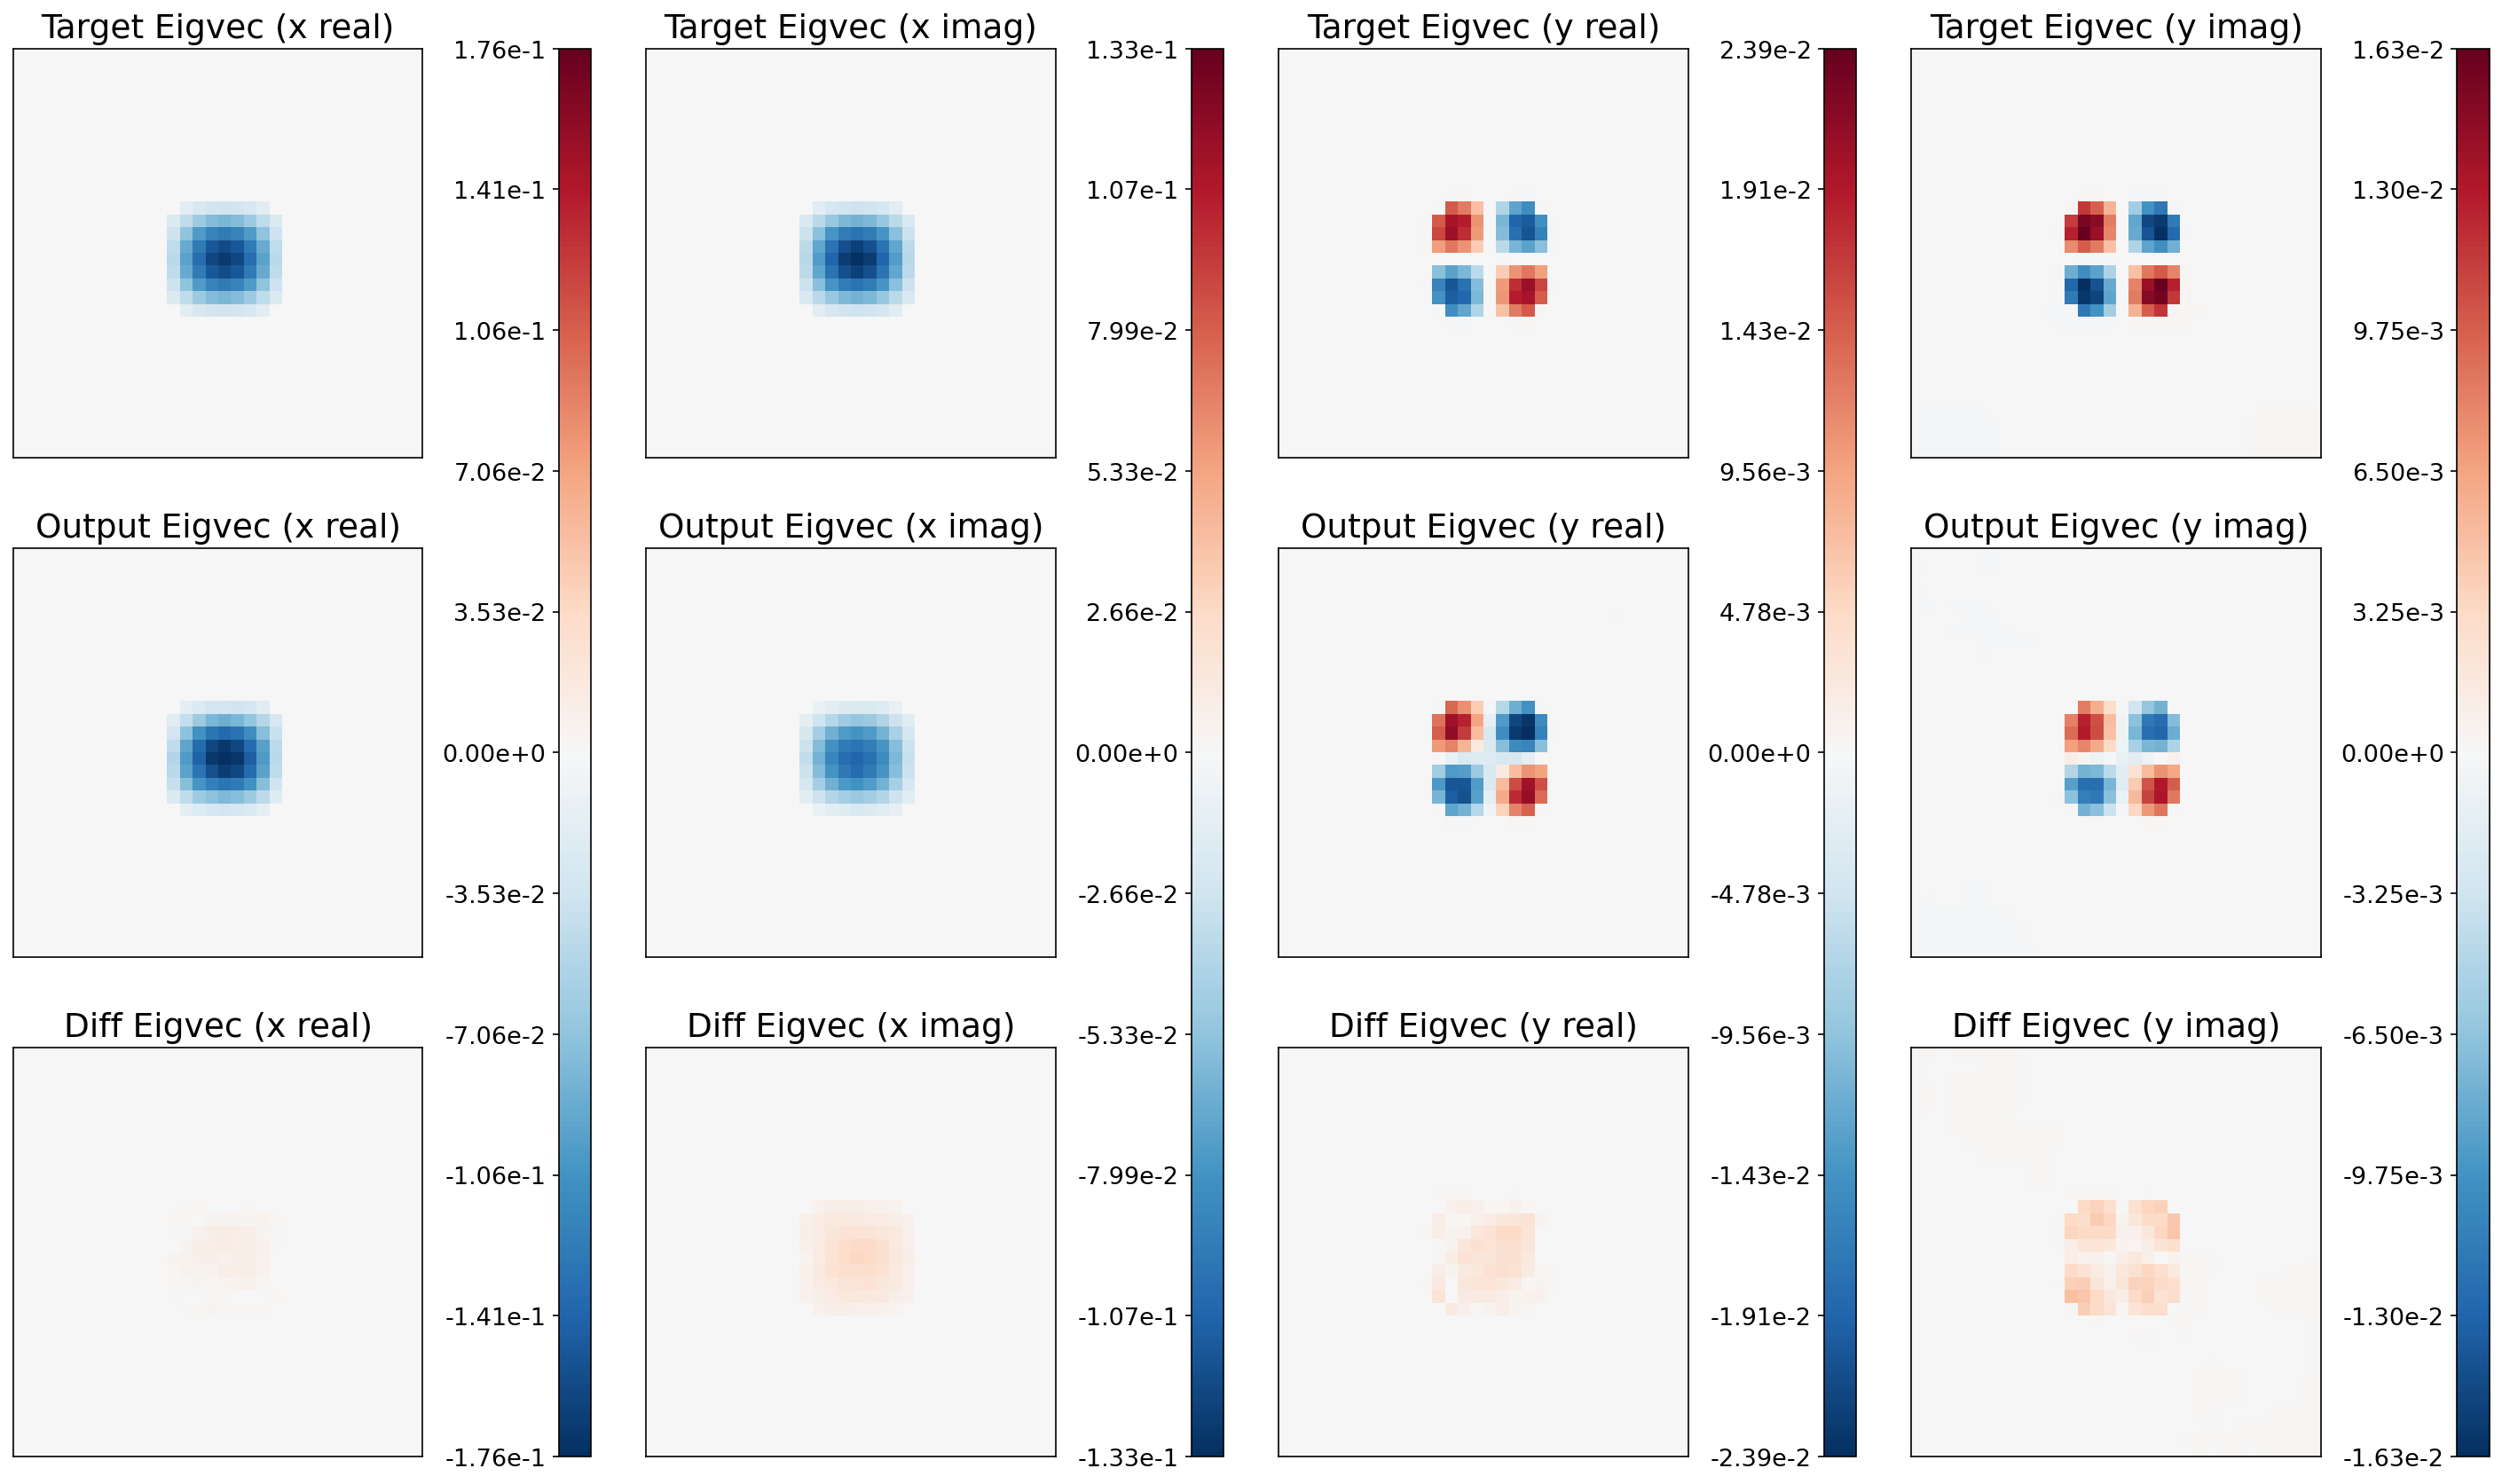
\includegraphics[width=\textwidth]{Figures/Fields C/c_test_nmae_p25_g452_w224_b1_fields.png}
        \caption{Output predictions at the 25th percentile of performance for unseen continuous valued geometries. The first row are target fields, followed by prediction fields on the second row, and difference fields on the third. At the 25th percentile, prediction outcomes are already fairly good, with accurate representations of scale and structure.}
        \label{fig:c_p25_output}
    \end{subfigure}
\end{figure}

\begin{figure}[H]
    \centering
    \begin{subfigure}[c]{0.75\textwidth}
        \centering
        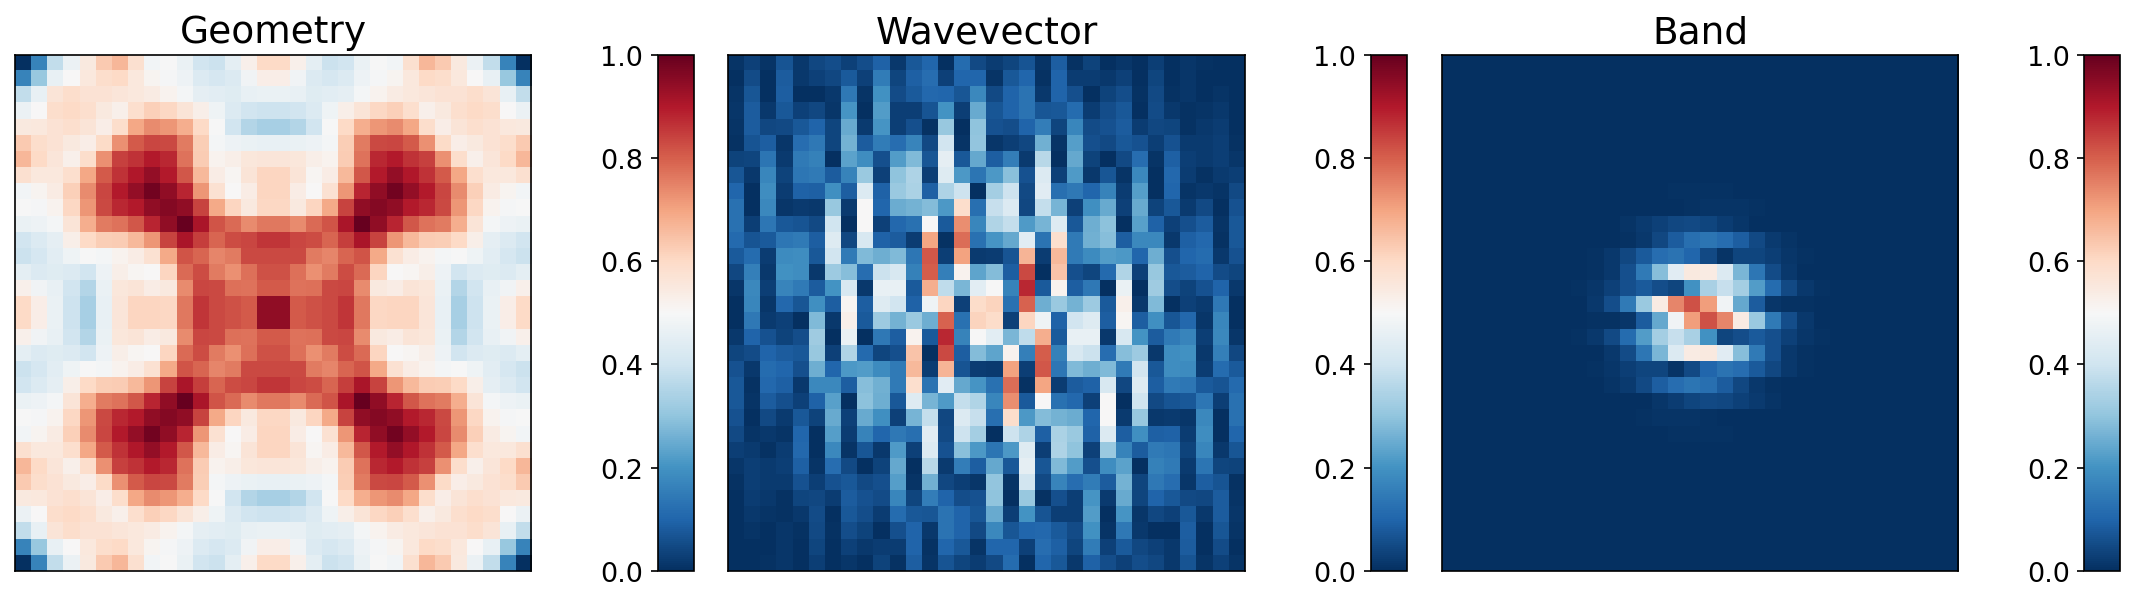
\includegraphics[width=\textwidth]{Figures/Fields C/c_test_nmae_p50_g183_w41_b3_input.png}
        \caption{Input sample at the 50th percentile of performance for unseen continuous valued geometries.}
        \label{fig:c_p50_input}
    \end{subfigure}
    \vspace{1em}
    \begin{subfigure}[c]{\textwidth}
    \centering
        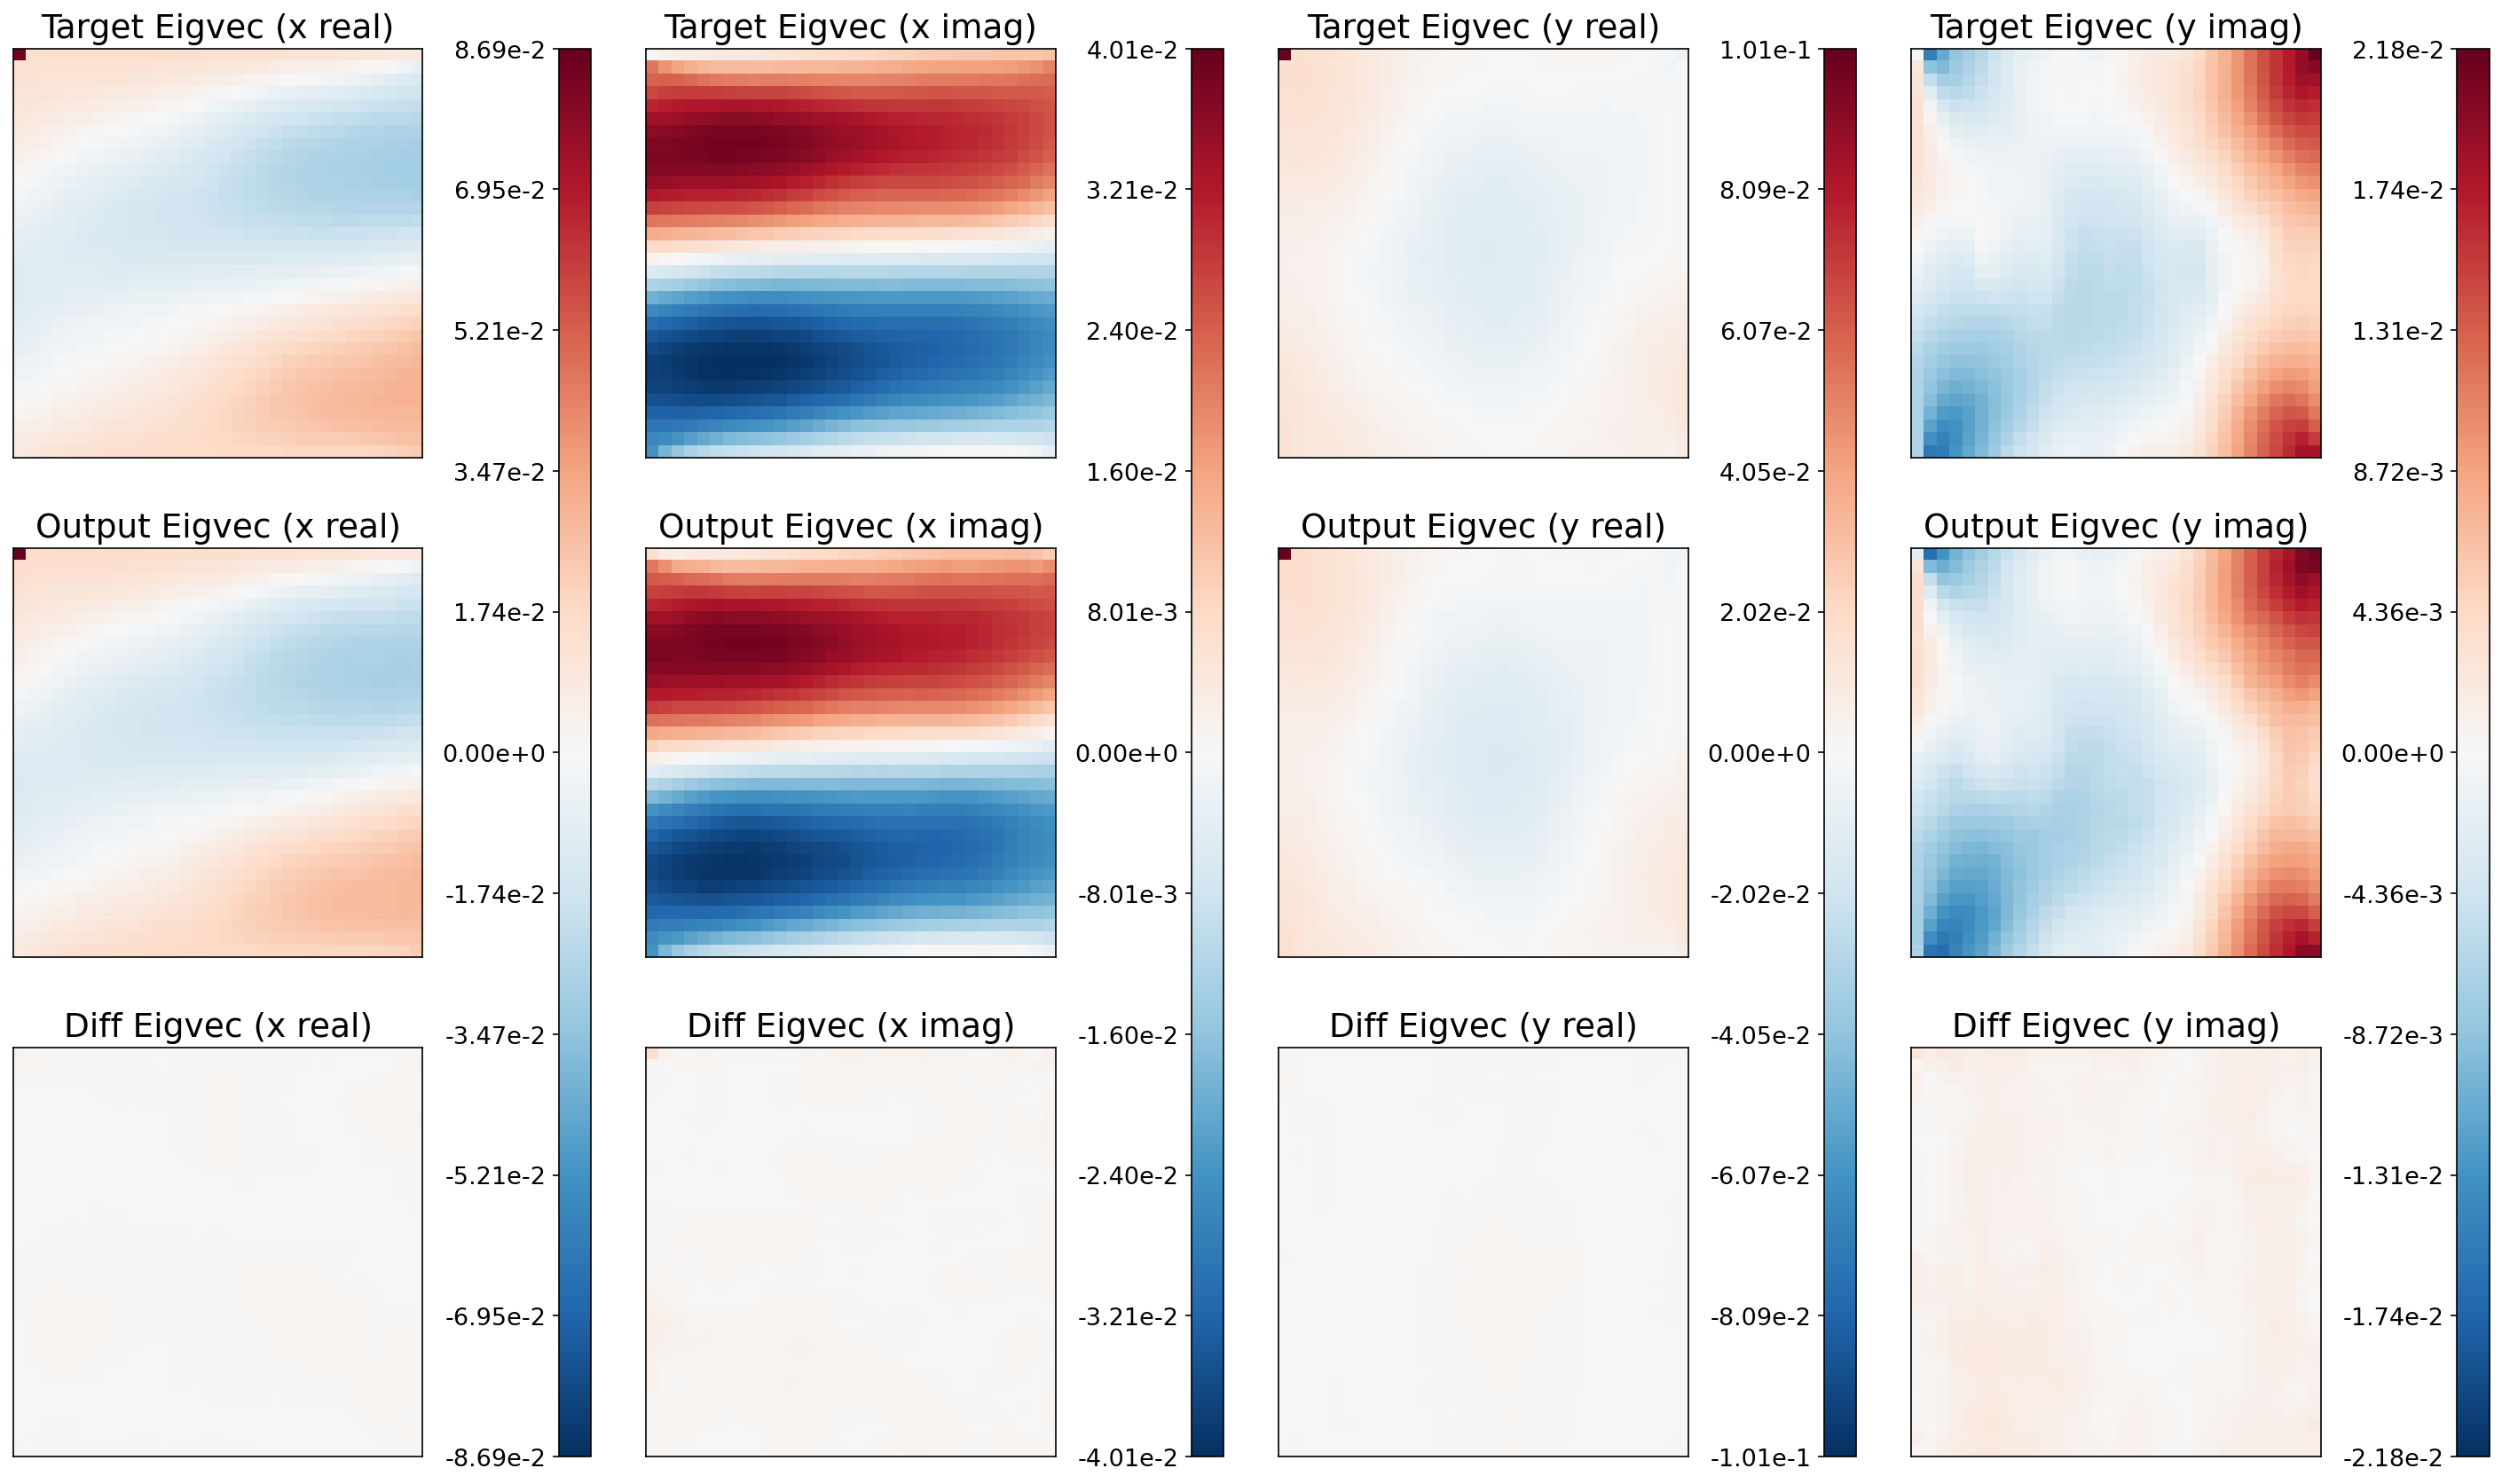
\includegraphics[width=\textwidth]{Figures/Fields C/c_test_nmae_p50_g183_w41_b3_fields.png}
        \caption{Output predictions at the 50th percentile of performance for unseen continuous valued geometries. The first row are target fields, followed by prediction fields on the second row, and difference fields on the third. Predictions are able to consistently capture complex structures without graininess.}
        \label{fig:c_p50_output}
    \end{subfigure}
\end{figure}

\begin{figure}[H]
    \centering
    \begin{subfigure}[c]{0.75\textwidth}
        \centering
        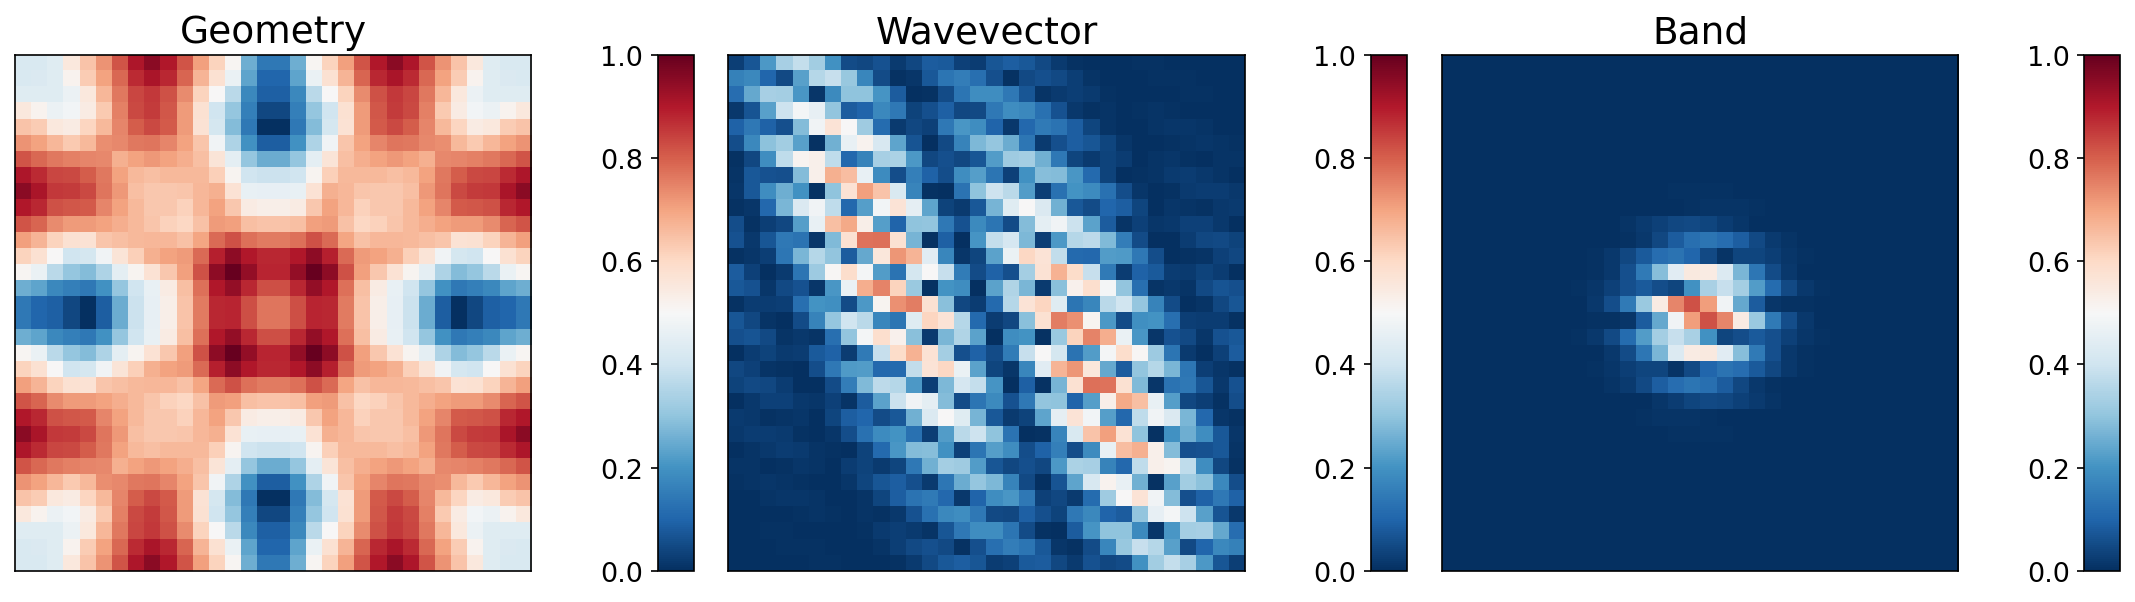
\includegraphics[width=\textwidth]{Figures/Fields C/c_test_nmae_p75_g279_w229_b3_input.png}
        \caption{Input sample at the 75th percentile of performance for unseen continuous valued geometries.}
        \label{fig:c_p75_input}
    \end{subfigure}
    \vspace{1em}
    \begin{subfigure}[c]{\textwidth}
    \centering
        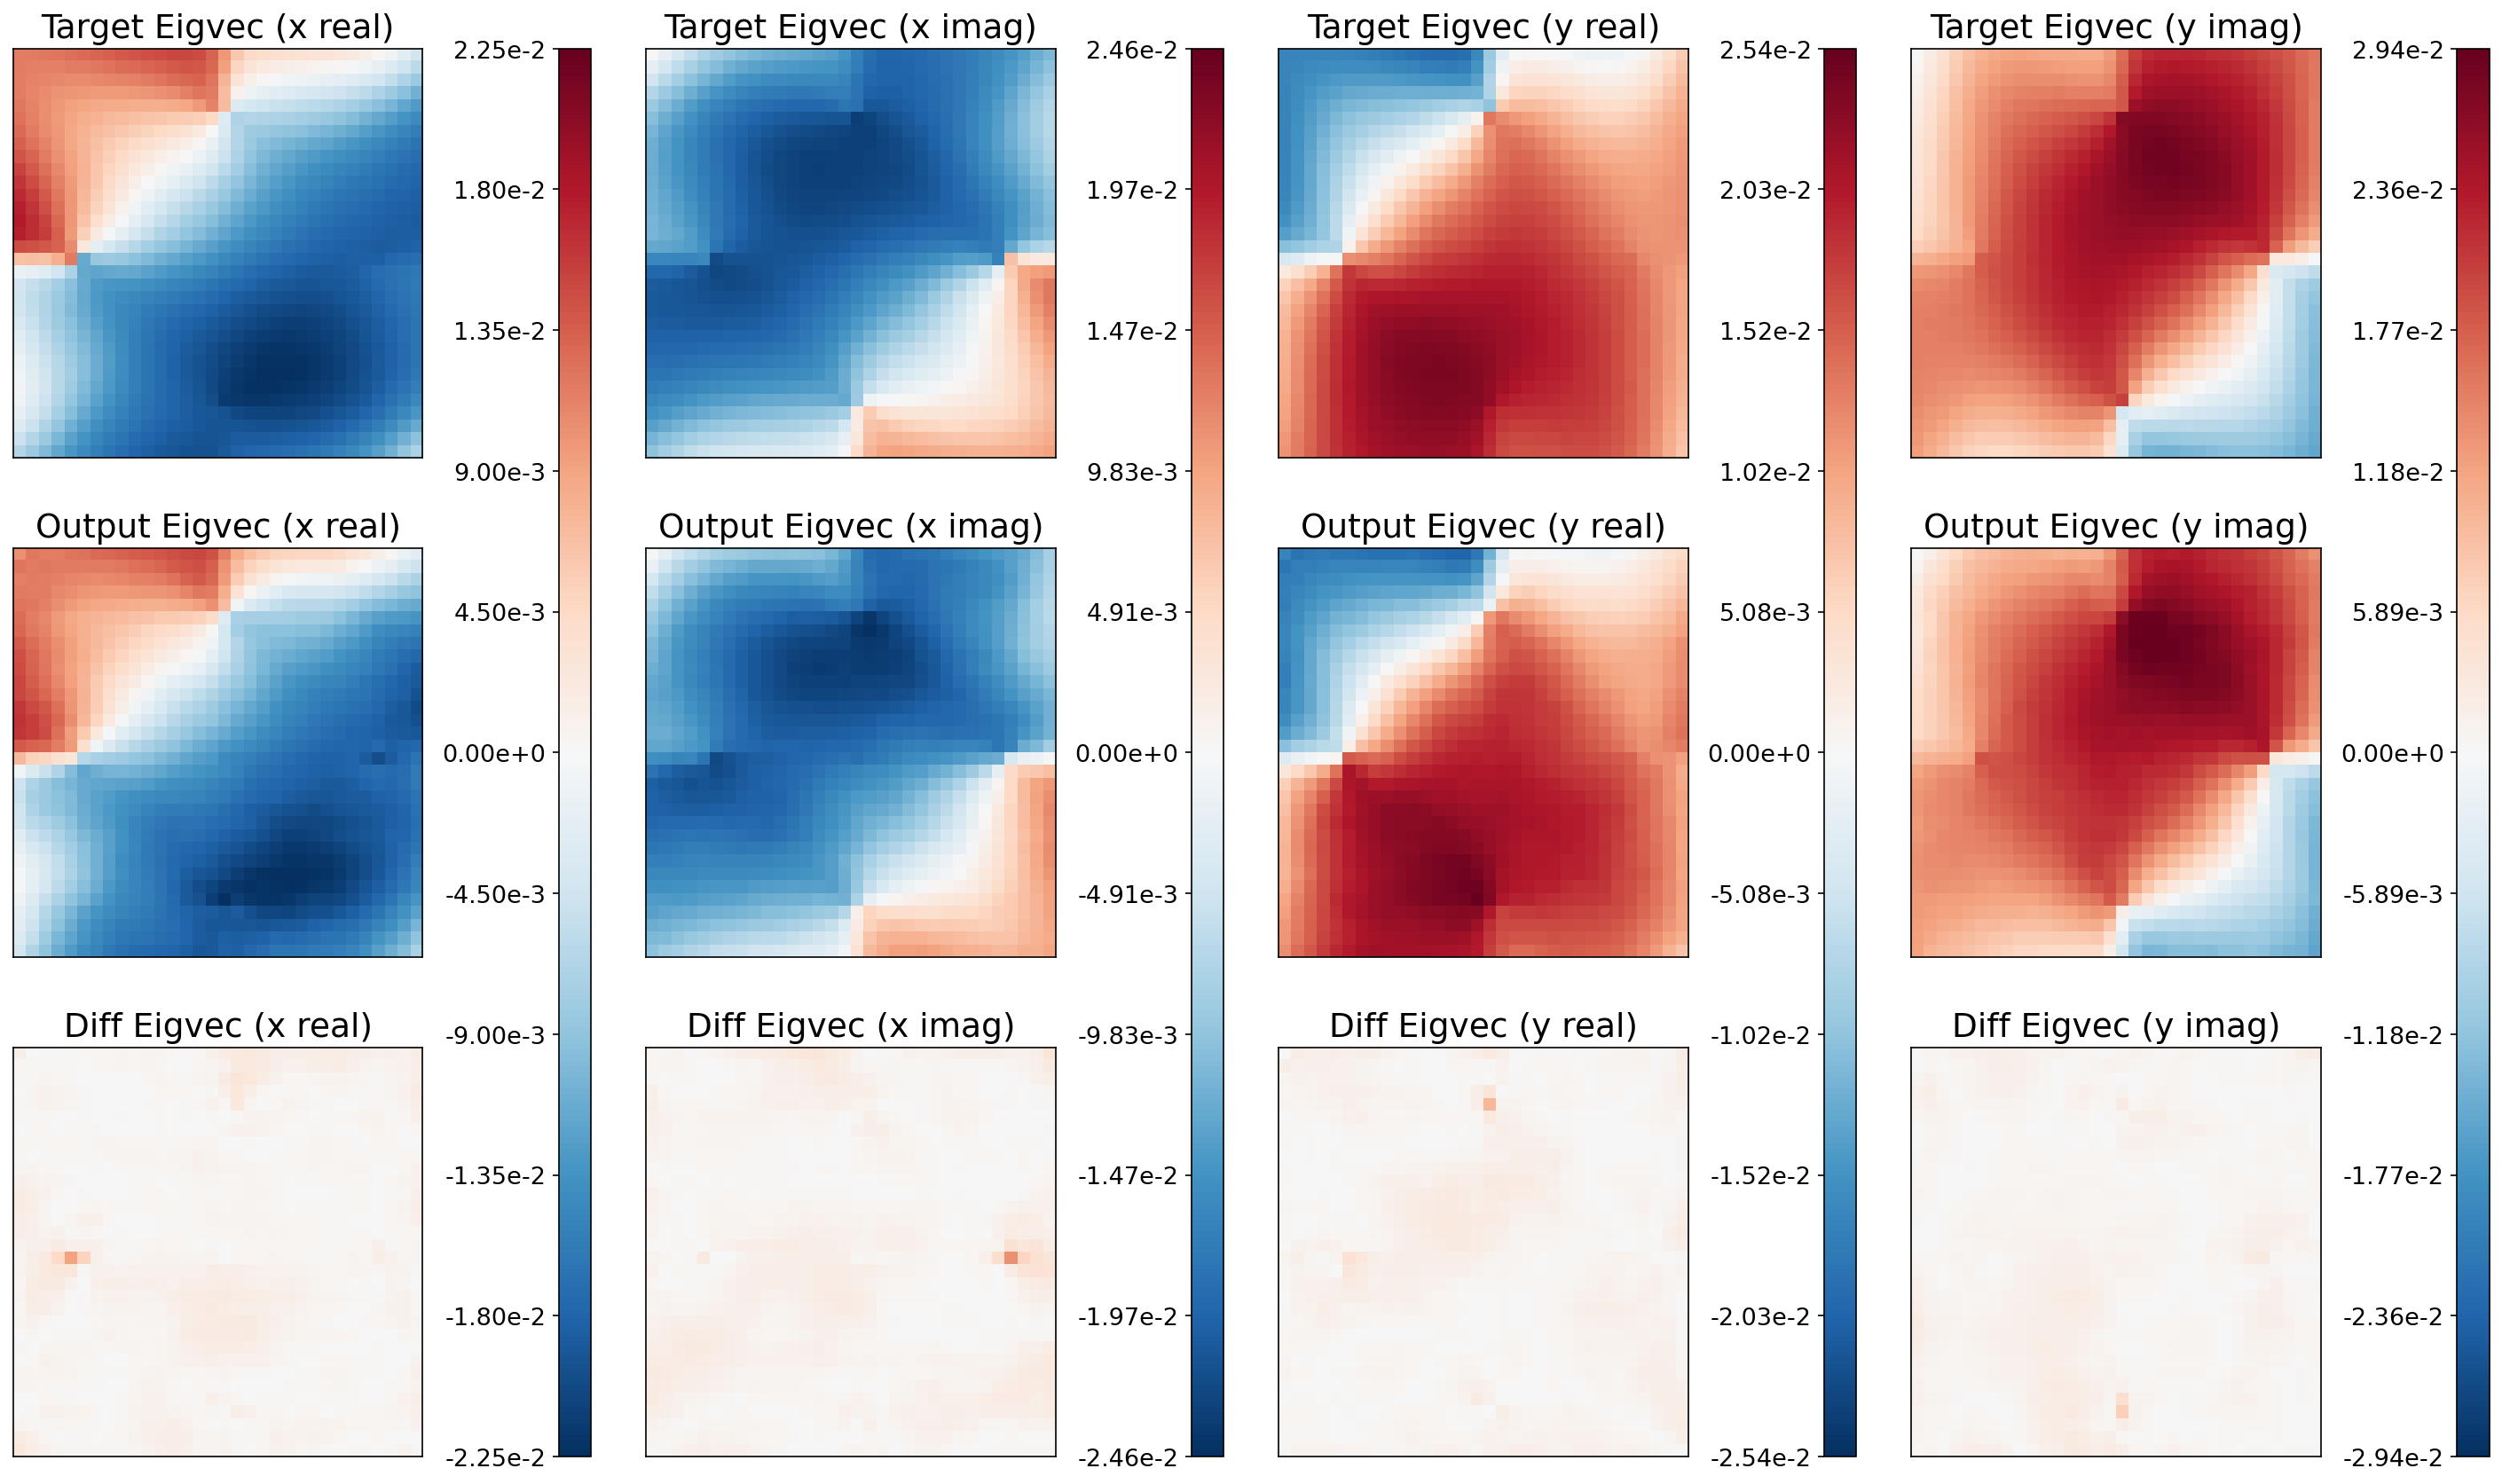
\includegraphics[width=\textwidth]{Figures/Fields C/c_test_nmae_p75_g279_w229_b3_fields.png}
        \caption{Output predictions at the 75th percentile of performance for unseen continuous valued geometries. The first row are target fields, followed by prediction fields on the second row, and difference fields on the third. At this point, the target and prediction are virtually indistinguishable by eye.}
        \label{fig:c_p75_output}
    \end{subfigure}
\end{figure}
These results demonstrate that with wavelet encodings, the FNO model performs well on continuous geometries, faithfully reproducing the displacement fields in most cases. Model predictions in the top three quartiles match targets well in structure and scale, with decreasing average pixel relative errors in the scale of $~10^{-2}$ smoothly decreasing down to $~10^{-4}$ with increasing percentile performance. (See Figure \ref{fig:disp_loss_histogram_continuous} for more detailed statistics.)

\subsubsection{Discrete Geometries}
\begin{figure}[H]
    \centering
    \begin{subfigure}[c]{\textwidth}
        \centering
        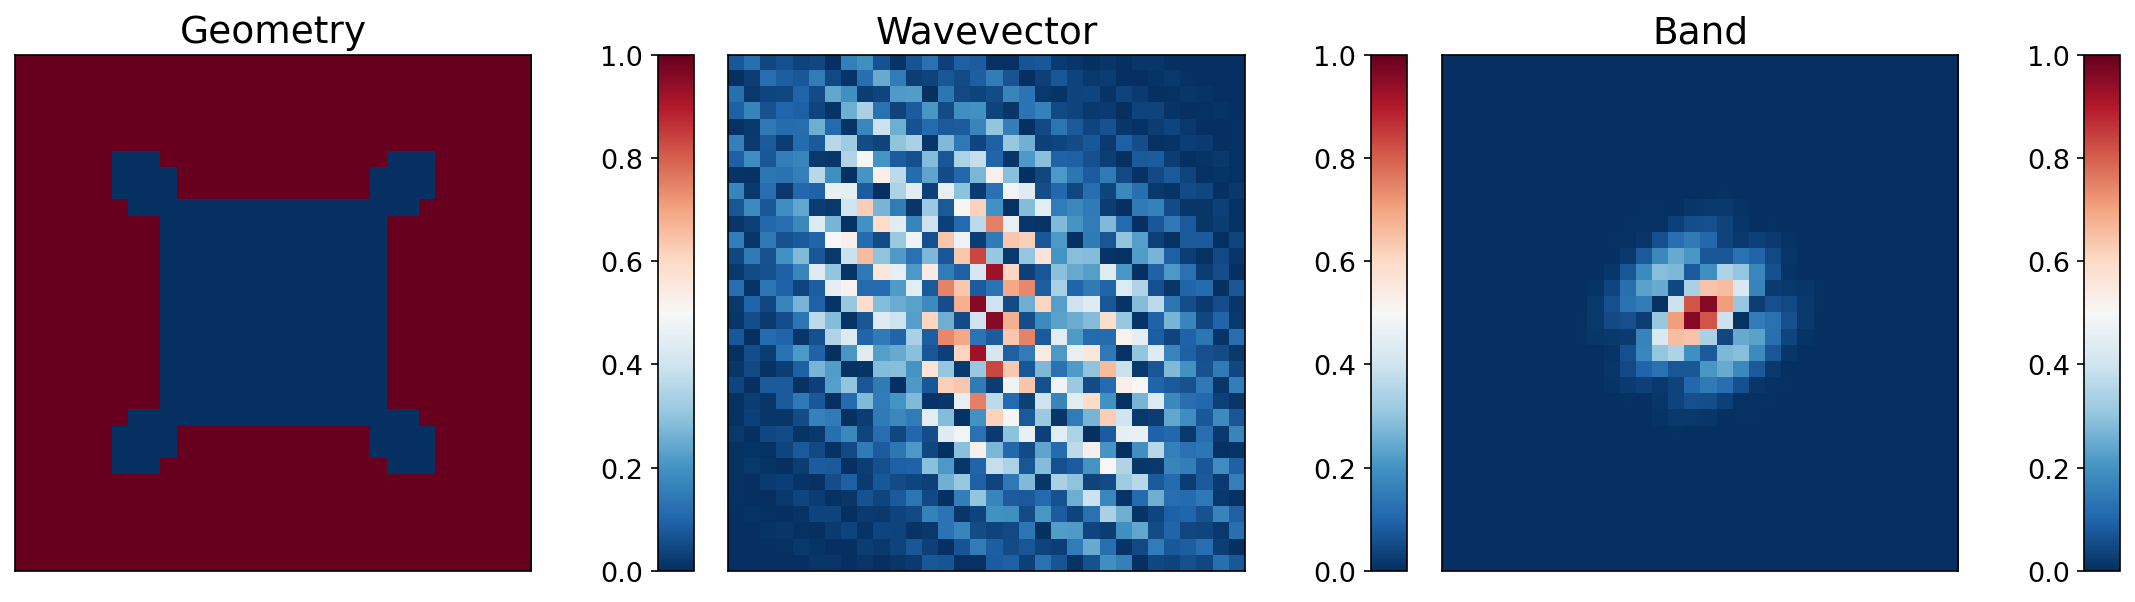
\includegraphics[width=0.75\textwidth]{Figures/Fields B/b_test_nmae_p25_g283_w234_b1_input.png}
        \caption{Input sample at the 25th percentile of performance for unseen discrete valued geometries.}
        \label{fig:b_p25_input}
    \end{subfigure}
    \vspace{1em}
    \begin{subfigure}[c]{\textwidth}
    \centering
        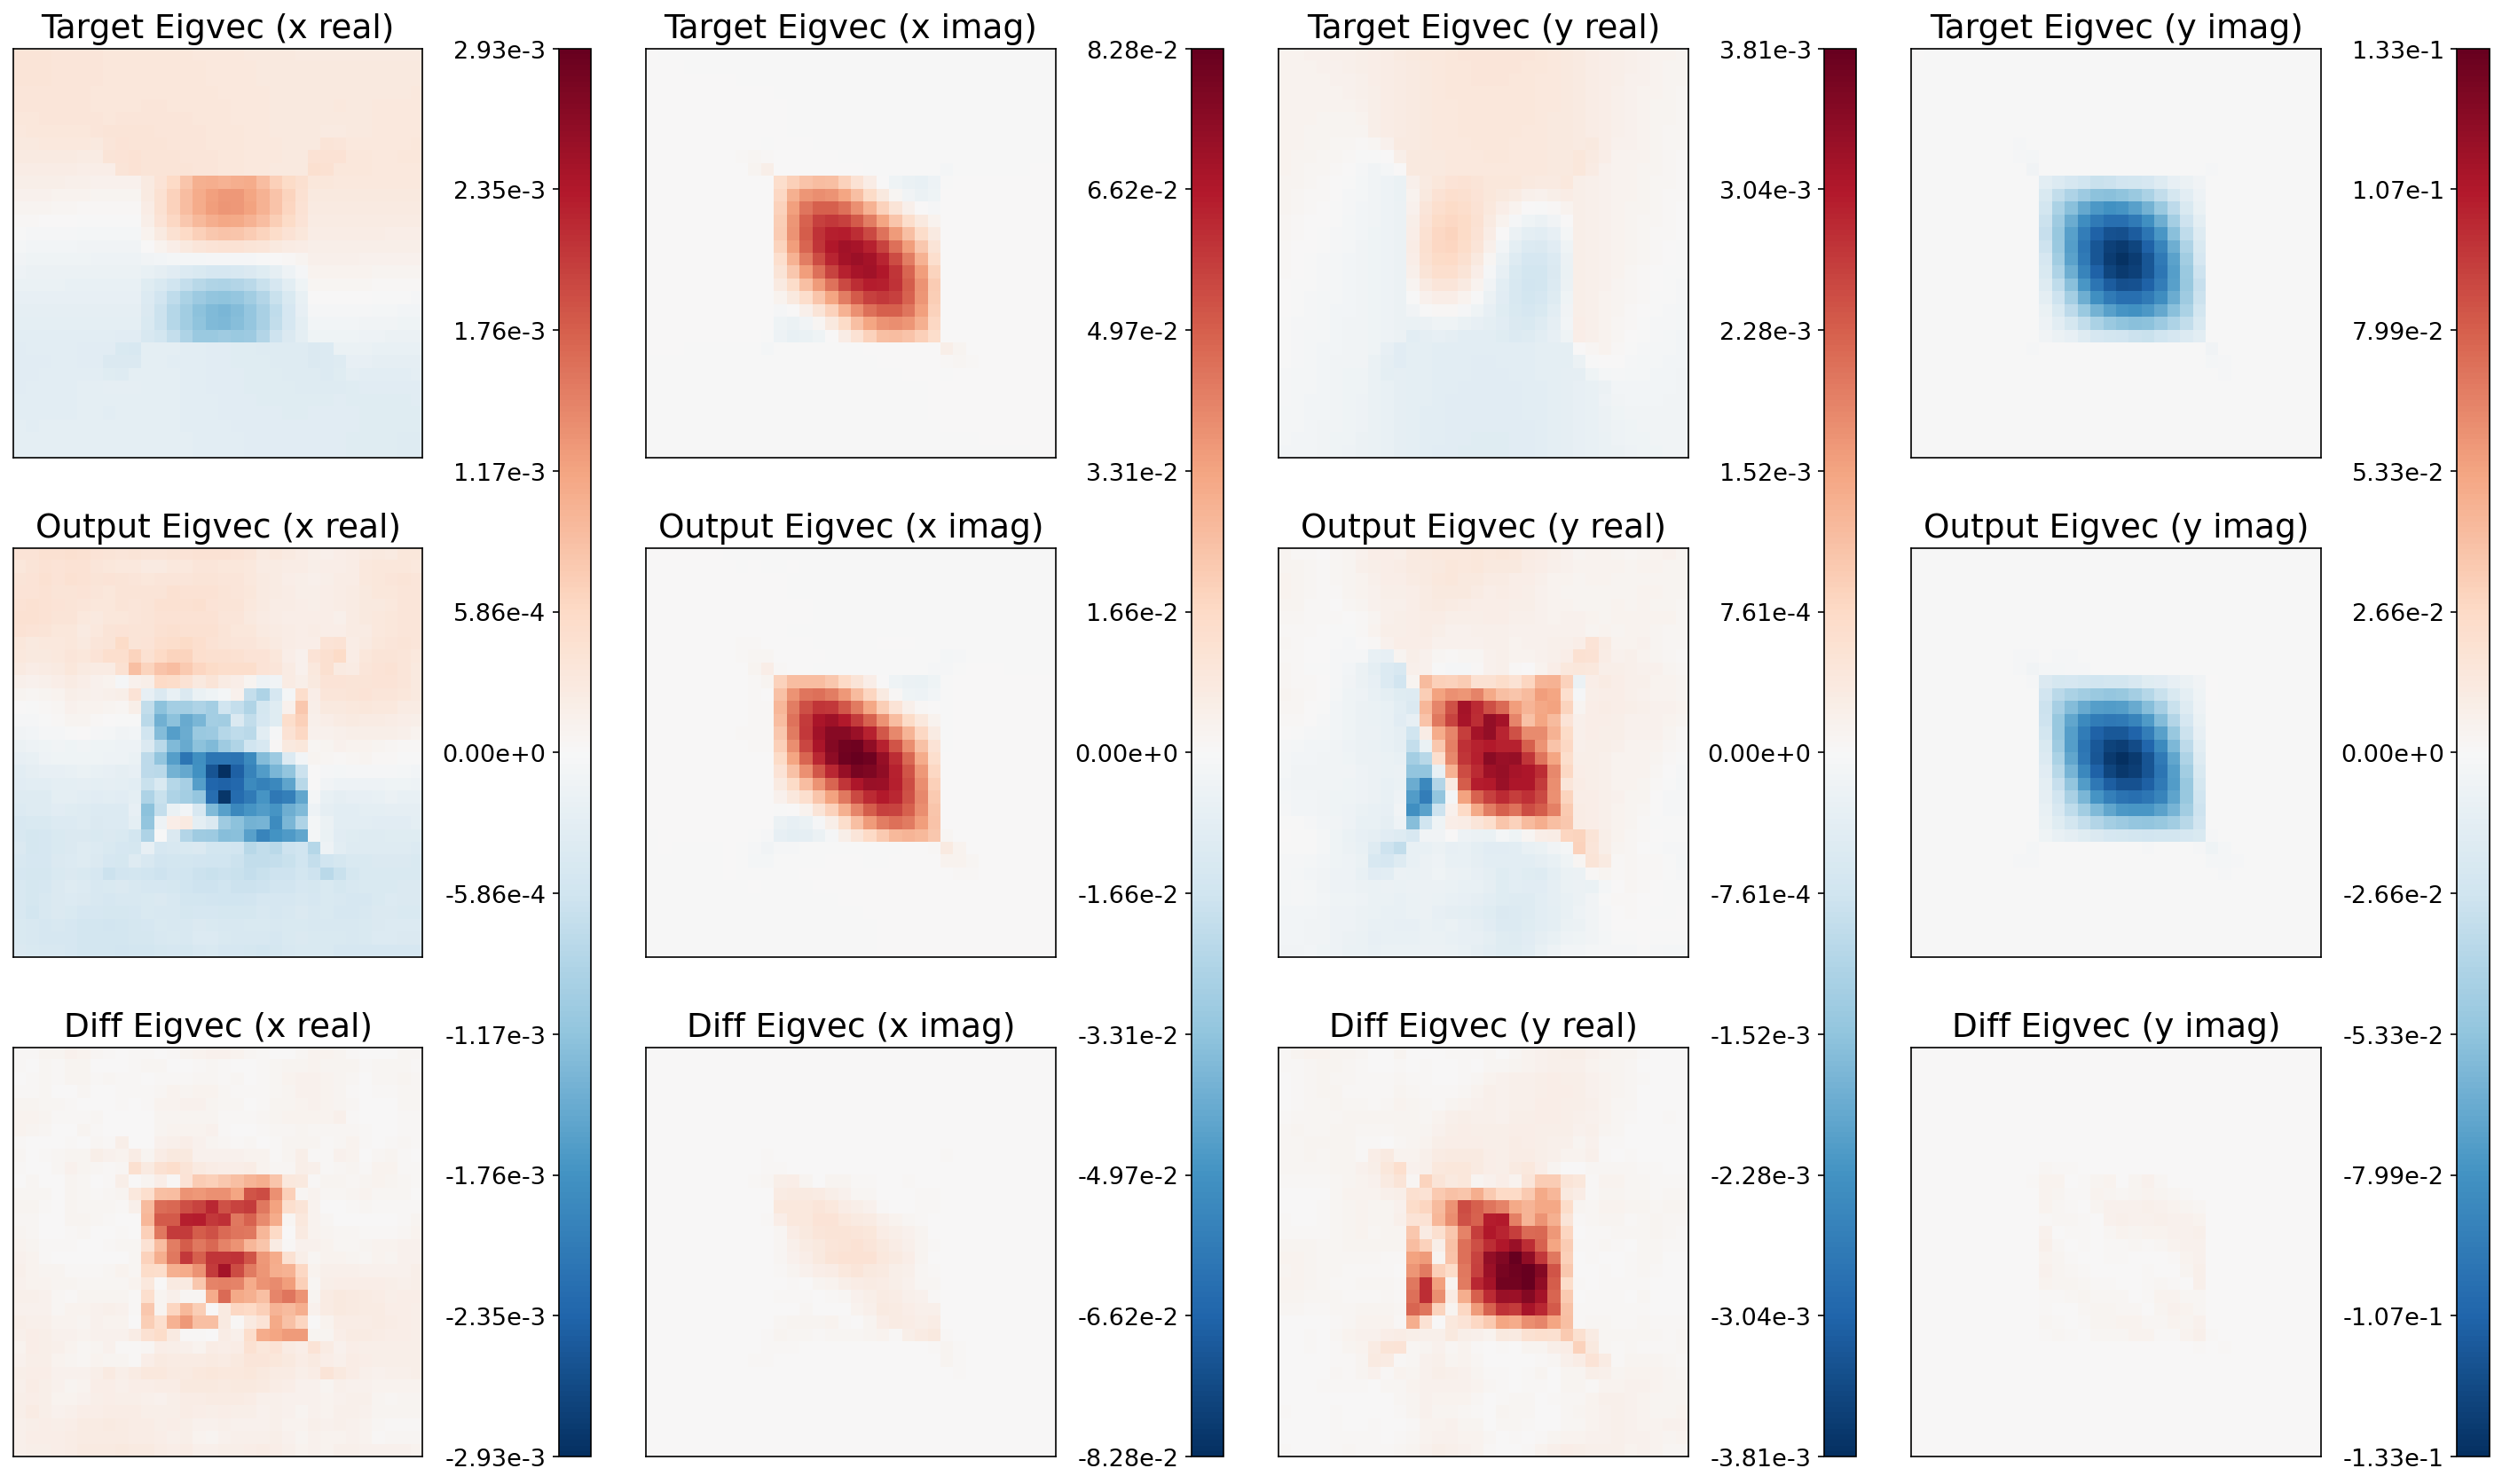
\includegraphics[width=\textwidth]{Figures/Fields B/b_test_nmae_p25_g283_w234_b1_fields.png}
        \caption{Output predictions at the 25th percentile of performance for unseen discrete valued geometries. The first row are target fields, followed by prediction fields on the second row, and difference fields on the third. Due to the nature of the loss function training, for this particular sample, the model would have prioritized the two imaginary displacement fields, because they are 1 to 2 orders of magnitude larger in scale compared to the two real displacement fields. In other words, absolute error is low at this point, but relative error is not for some channels of small scale than other channels. (Note that the colorbars for each column are independently scaled.)}
        \label{fig:b_p25_output}
    \end{subfigure}
\end{figure}

\begin{figure}[H]
    \centering
    \begin{subfigure}[c]{\textwidth}
        \centering
        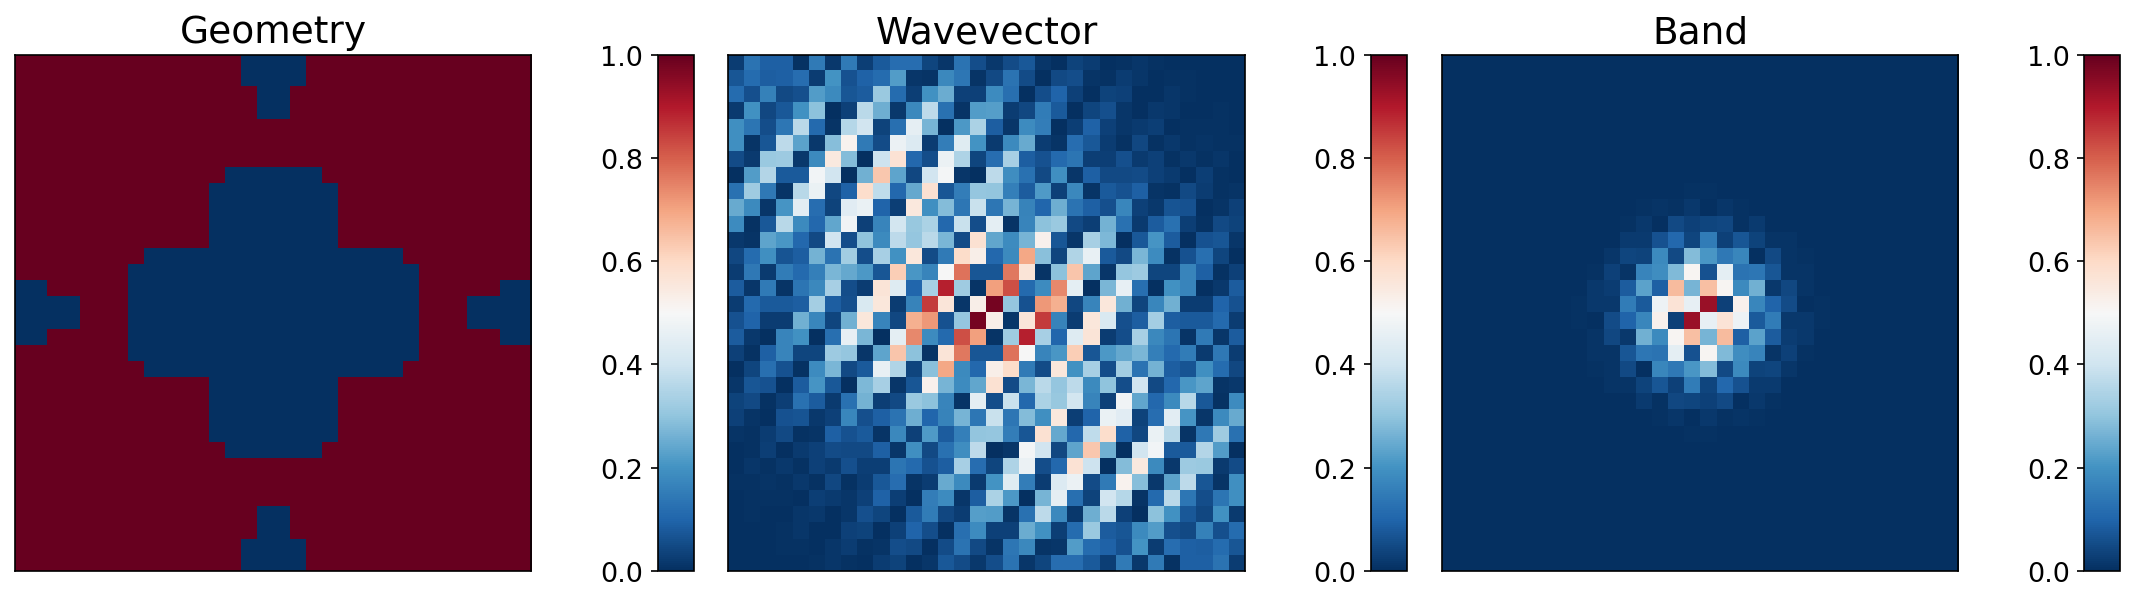
\includegraphics[width=0.75\textwidth]{Figures/Fields B/b_test_nmae_p50_g550_w257_b4_input.png}
        \caption{Input sample at the 50th percentile of performance for unseen discrete valued geometries.}
        \label{fig:b_p50_input}
    \end{subfigure}
    \vspace{1em}
    \begin{subfigure}[c]{\textwidth}
    \centering
        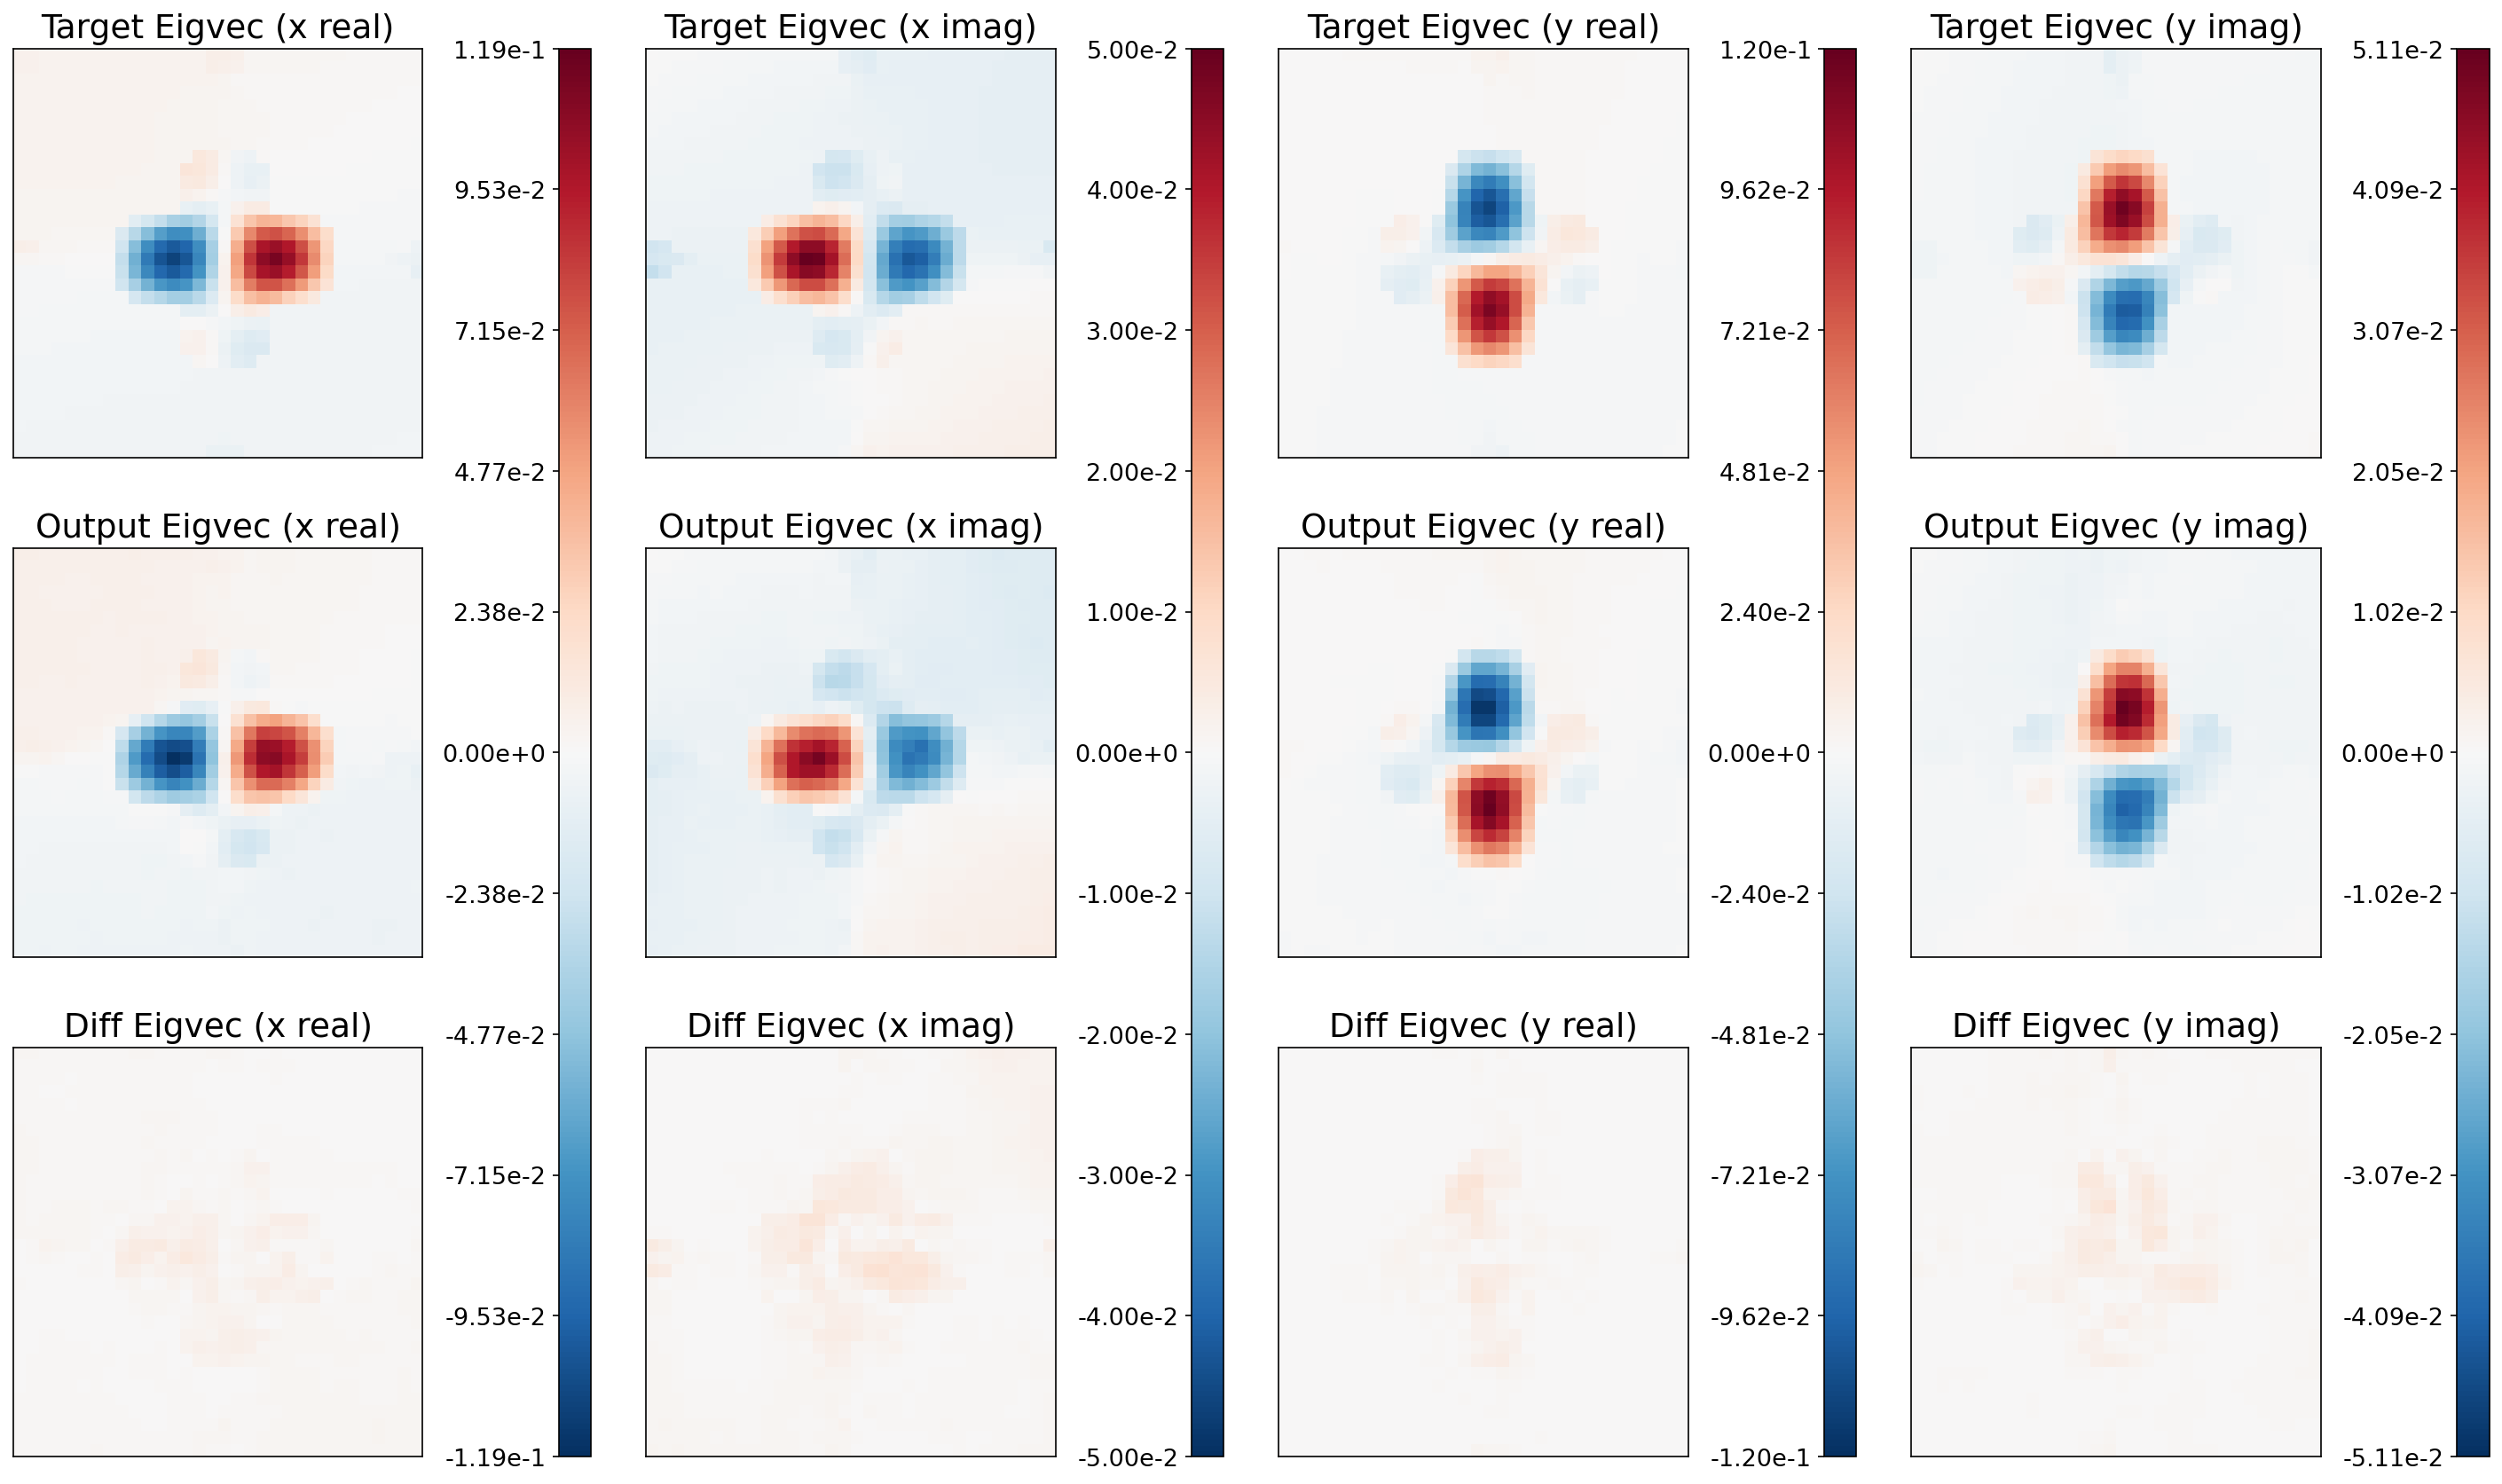
\includegraphics[width=\textwidth]{Figures/Fields B/b_test_nmae_p50_g550_w257_b4_fields.png}
        \caption{Output predictions at the 50th percentile of performance for unseen discrete valued geometries. The first row are target fields, followed by prediction fields on the second row, and difference fields on the third. At this point, absolute and relative errors are low and there is high agreement in structural and scale between targets and predictions.}
        \label{fig:b_p50_output}
    \end{subfigure}
\end{figure}

\begin{figure}[H]
    \centering
    \begin{subfigure}[c]{\textwidth}
        \centering
        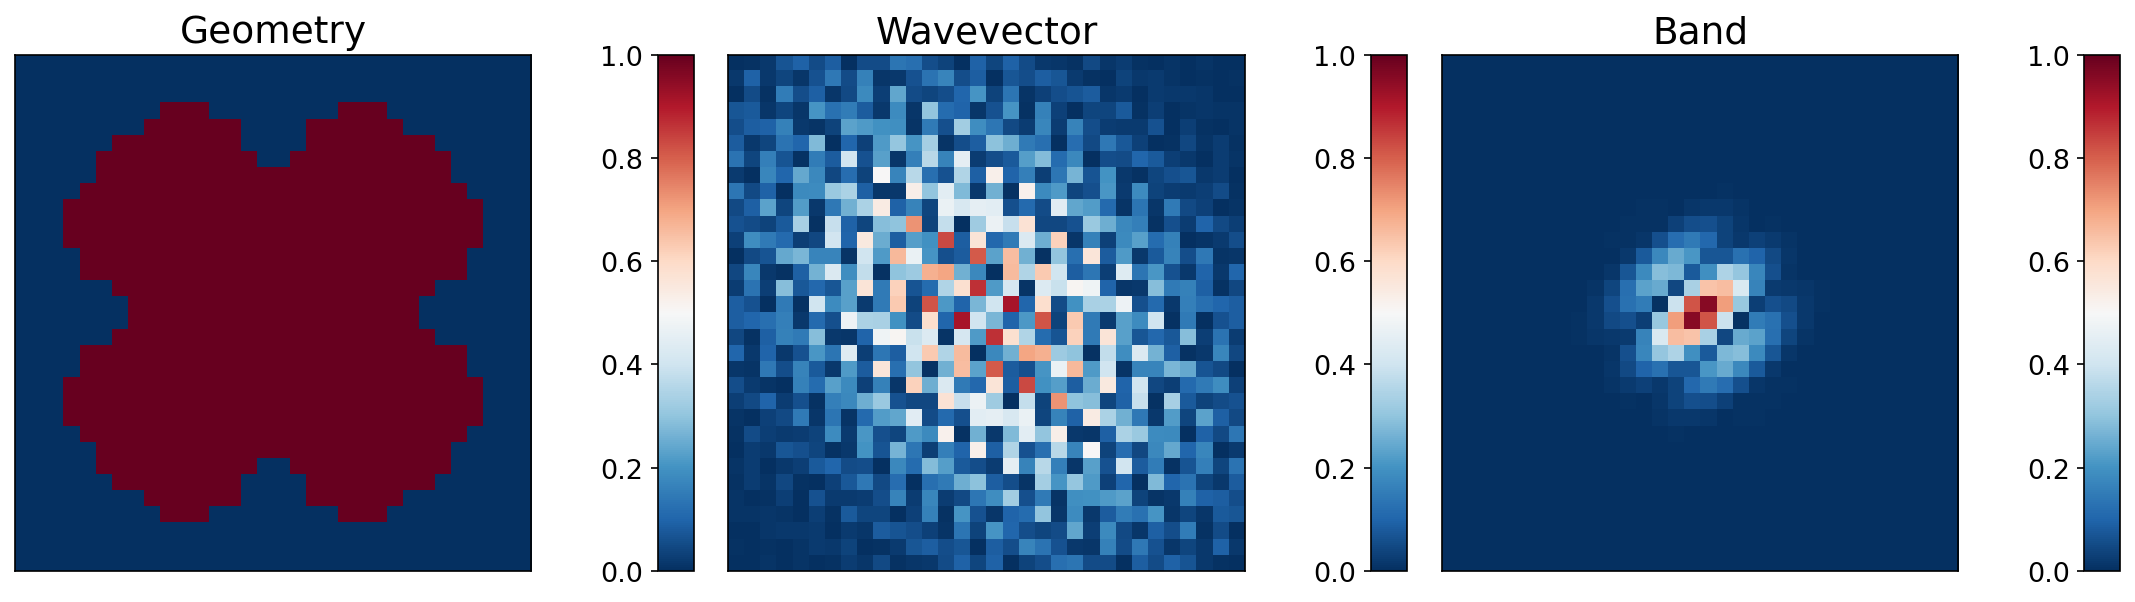
\includegraphics[width=0.75\textwidth]{Figures/Fields B/b_test_nmae_p75_g234_w145_b1_input.png}
        \caption{Input sample at the 75th percentile of performance for unseen discrete valued geometries.}
        \label{fig:b_p75_input}
    \end{subfigure}
    \vspace{1em}
    \begin{subfigure}[c]{\textwidth}
    \centering
        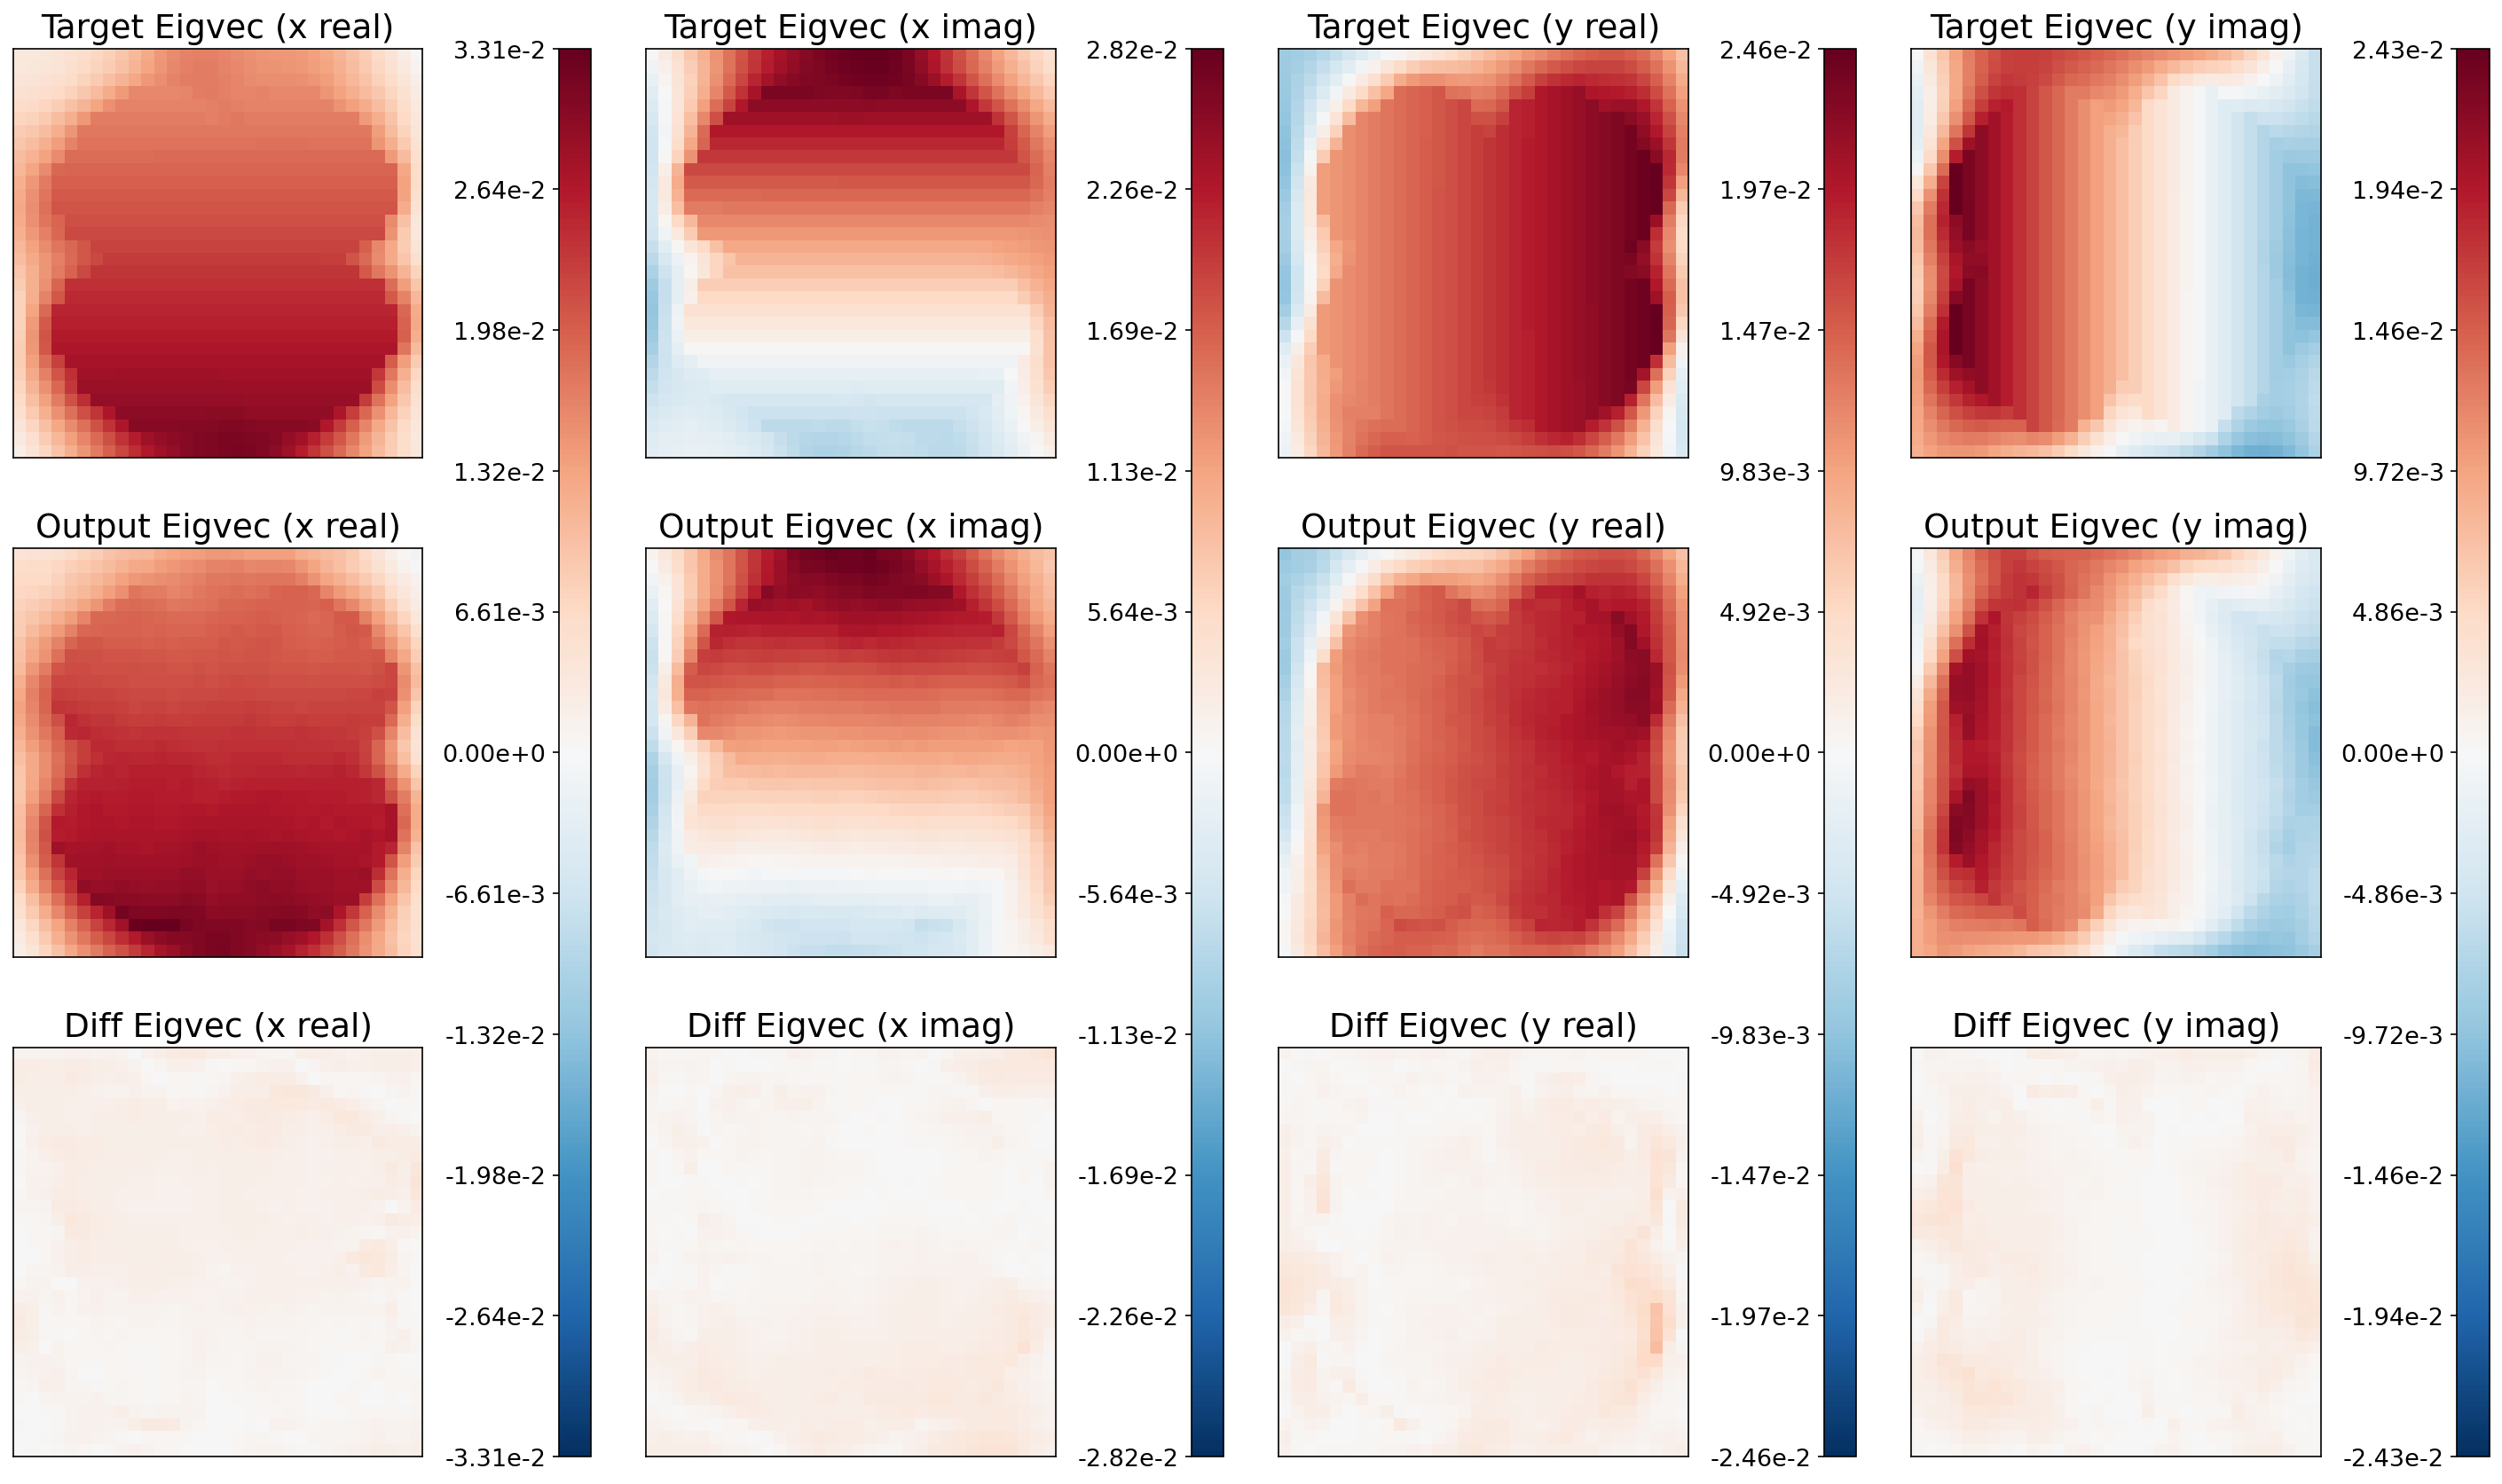
\includegraphics[width=\textwidth]{Figures/Fields B/b_test_nmae_p75_g234_w145_b1_fields.png}
        \caption{Output predictions at the 75th percentile of performance for unseen discrete valued geometries. The first row are target fields, followed by prediction fields on the second row, and difference fields on the third. At this point, disagreements between targets and predictions become very hard to see by eye.}
        \label{fig:b_p75_output}
    \end{subfigure}
\end{figure}

Like with the continuous geometry case, these results demonstrate that with wavelet encodings, the FNO model performs well on discrete geometries, faithfully reproducing the displacement fields in most cases. Model predictions in the top three quartiles match targets well in structure and scale, with decreasing average pixel relative errors in the scale of $~10^{-2}$ smoothly decreasing down to $~10^{-4}$ with increasing percentile performance. (See Figure \ref{fig:disp_loss_histogram_discrete} for more detailed statistics.)

\subsubsection{Continuous Versus Discrete Performance}
The model being able to simultaneously predict well on both continuous and discrete geometries is a non-trivial and important takeaway for the capabilities of FNOs with paired with wavelet encodings. Prior encoding strategies of constant fields and sinusoidal fields delivered far worse results with grainy structures or mode collapse issues because conditioning constants (wavevector and band) information could not propagate well through the spectral branch of the FNO layers. The performance over all unseen samples in the test set are shown in \ref{fig:disp_loss_histograms}. 

The poorer performance on binarized geometries is consistent with basic operator-learning theory. Continuous material fields lie in smoother function classes, whereas binary two-phase designs contain jump discontinuities with nonexistent derivatives at material interfaces. Since an FNO approximates the FEA operator $\mathcal{G}: \mathcal{U}\to\mathcal{V}$ through truncated Fourier representations, it is naturally advantaged when both inputs and outputs are comparatively smooth. Discrete geometries thus perform worse due to sharp boundaries, localized gradients, and broadband high-wavenumber content that are poorly captured on a fixed $32\times32$ grid and are mismatched to smooth wavelet encodings. Additionally, because continuous geometries have a greater tendency to have large sections of fields with zero or low displacements, a small spike is seen in relative error performance due to the near zero displacements which results in a small denominator.

These results indicate two important takeaways. The first is that it is possible for FNOs with wavelet encodings to learn multiple deformation modes for each geometry which the user can toggle between arbitrarily by setting the wavevector and band inputs. This is to our knowledge the first demonstration of FNOs on solving eigenvalue PDEs. The second, is that it is possible for that same model to simultaneously learn very different distributions of geometries (continuous valued and discrete valued), indicating it might be possible to distill out a generalized understanding of the PDE itself independent of geometry distributions and statistical artifacts. This is a possible subject for future work.

\begin{figure}[H]
    \centering
    \begin{subfigure}[t]{0.49\textwidth}
        \centering
        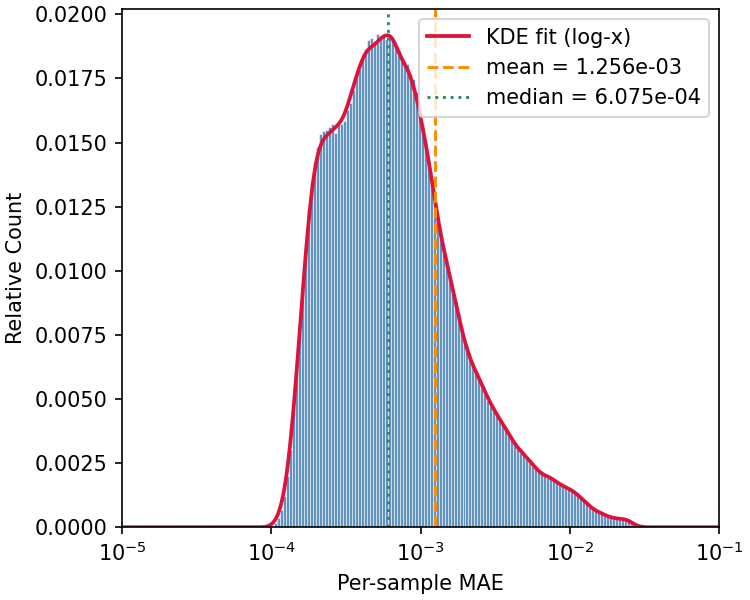
\includegraphics[width=\textwidth]{Figures/Statistics/displacement_loss_histogram_mae_c_test.png}
        \caption{Performance histogram for continuous geometries.}
        \label{fig:disp_loss_histogram_continuous}
    \end{subfigure}
    \hfill
    \begin{subfigure}[t]{0.49\textwidth}
        \centering
        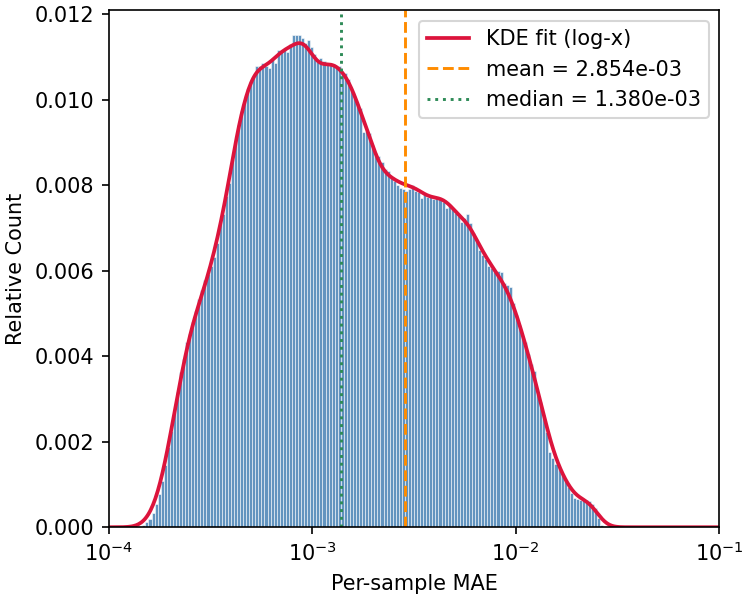
\includegraphics[width=\textwidth]{Figures/Statistics/displacement_loss_histogram_mae_b_test.png}
        \caption{Performance histogram for discrete geometries.}
        \label{fig:disp_loss_histogram_discrete}
    \end{subfigure}
    \caption{Comparison of relative prediction error distributions for continuous-valued and discrete metamaterial geometries for the same model. While there are some tail outliers, most samples fall within the range of $~10^{-2}$ to $~10^{-4}$, indicating that the same model is able to learn continuous and discrete geometry cases.}
    \label{fig:disp_loss_histograms}
\end{figure}

%%%%%%%%%%%%%%%%%%%%%%%%%%%%%%%%%%%%%%%%%%%%%%%%%%%%%%%%%%%%%%%%%%%%%%
\subsection{Dispersion Band Reconstruction}
\begin{figure}[H]
    \centering
    \begin{subfigure}[t]{0.32\textwidth}
        \centering
        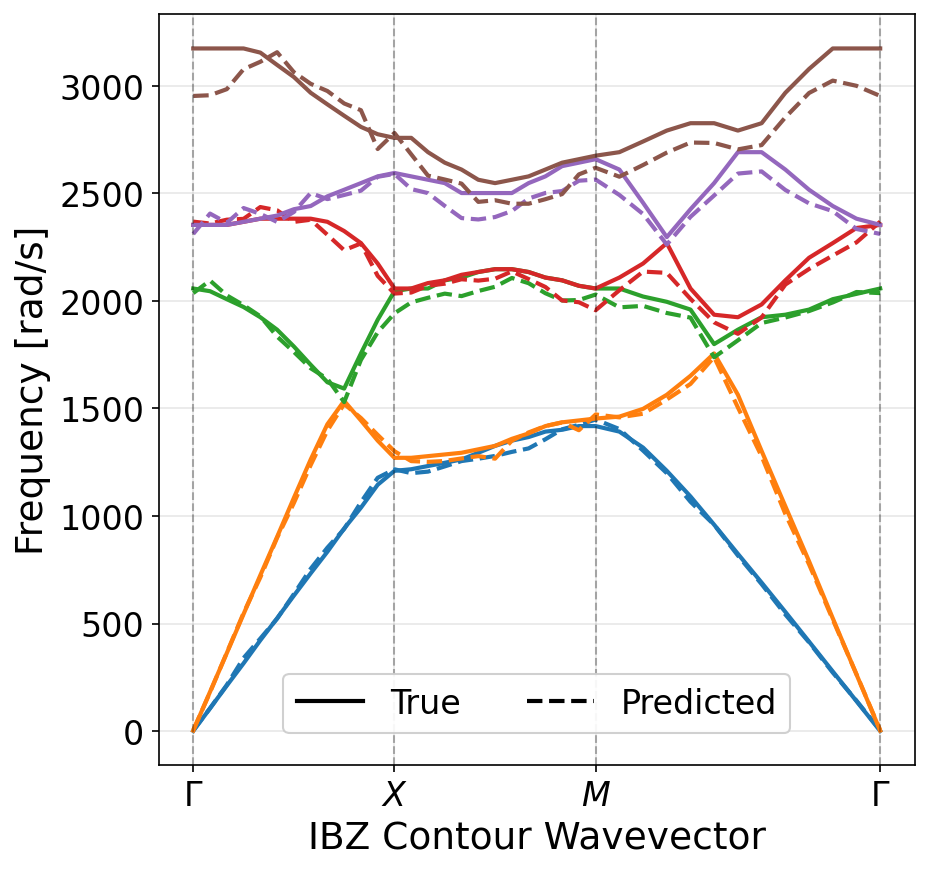
\includegraphics[width=\textwidth]{Figures/Dispersion C/NMAE753_NMSE730_g597.png}
        \caption{25th percentile performance.}
        \label{fig:dispersion_c_p25}
    \end{subfigure}
    \hfill
    \begin{subfigure}[t]{0.32\textwidth}
        \centering
        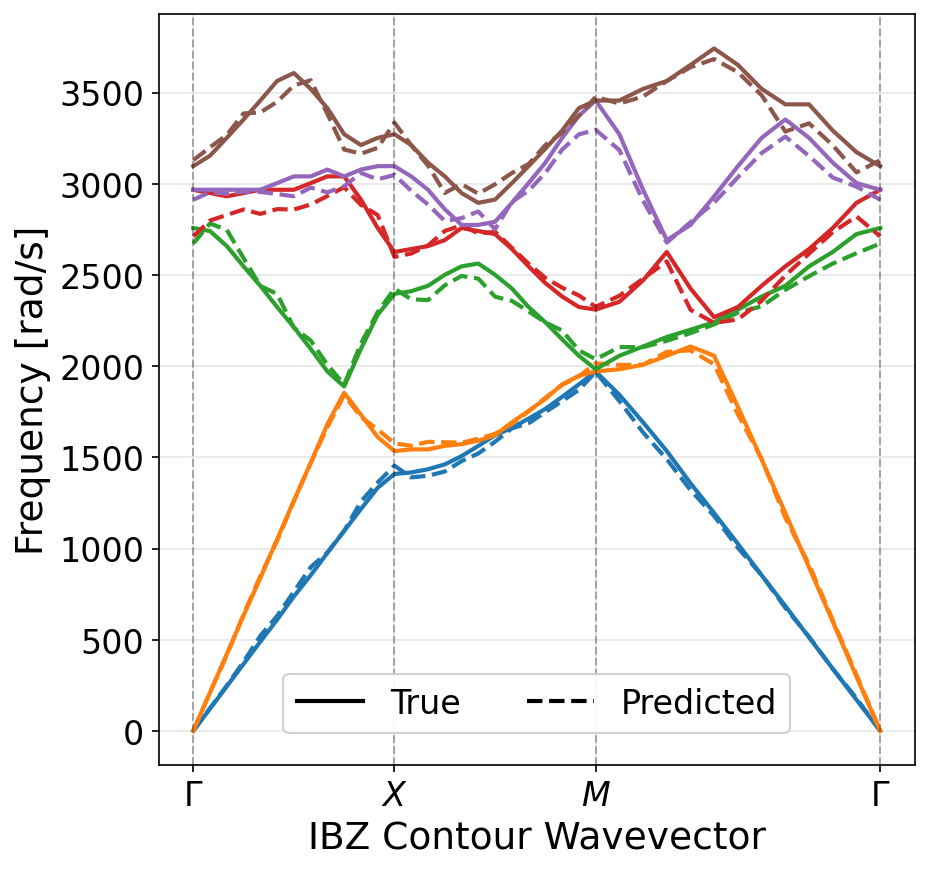
\includegraphics[width=\textwidth]{Figures/Dispersion C/NMAE502_NMSE443_g182.png}
        \caption{50th percentile performance.}
        \label{fig:dispersion_c_p50}
    \end{subfigure}
    \hfill
    \begin{subfigure}[t]{0.32\textwidth}
        \centering
        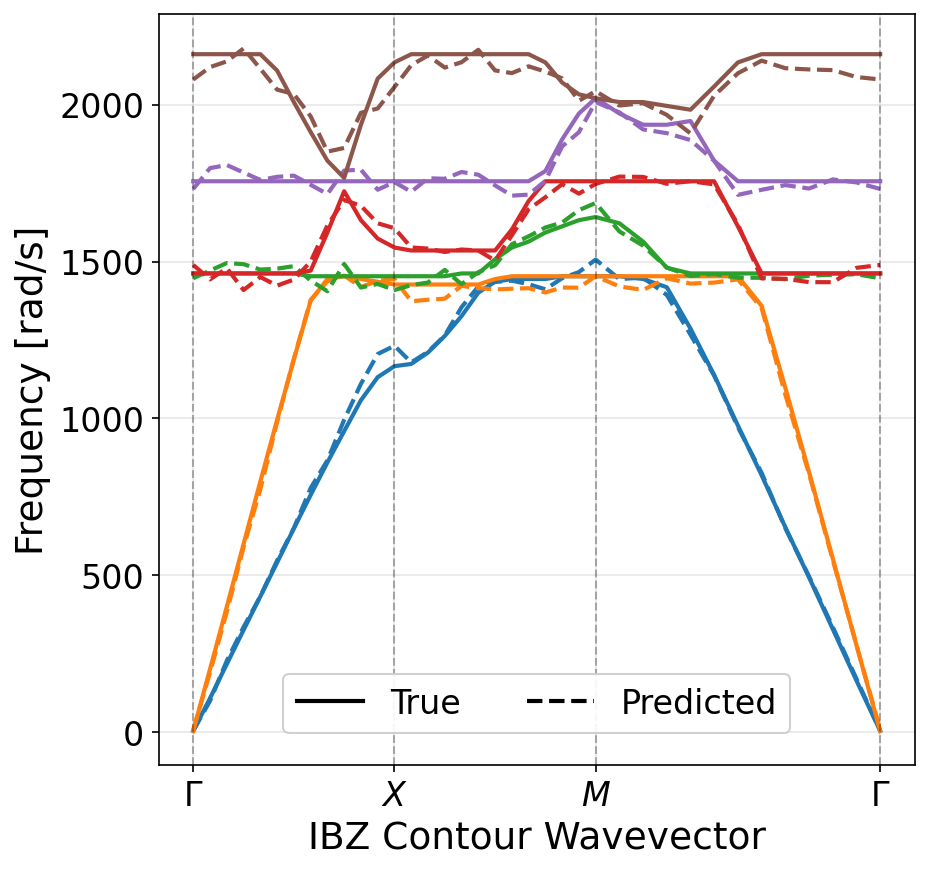
\includegraphics[width=\textwidth]{Figures/Dispersion C/NMAE250_NMSE250_g928.png}
        \caption{75th percentile performance.}
        \label{fig:dispersion_c_p75}
    \end{subfigure}
    \caption{Predicted and ground-truth dispersion bands for representative unseen continuous valued geometries spanning the 25th, 50th, and 75th percentiles of prediction performance.}
    \label{fig:dispersion_c_percentiles}
\end{figure}
These plots represent the eigenfrequency predictions of the model across all 325 wavevectors forming the half plane for continuous valued geometries, downselected to be the horizontal, vertical, and diagonal traversal of the IBZ. Note that because the encoding of the eigenfrequency into a field has a log operation (to allow the model to learn relationships at multiple scales), errors tend to be relative to the scale of the target, and thus higher bands may seem to be more deviant on a linear scale plot. Overall, the model performance is quite good at predictions in the encoded eigenfrequency, showing an average of < 1\% prediction error across all unseen samples.

\begin{figure}[H]
    \centering
    \begin{subfigure}[t]{0.32\textwidth}
        \centering
        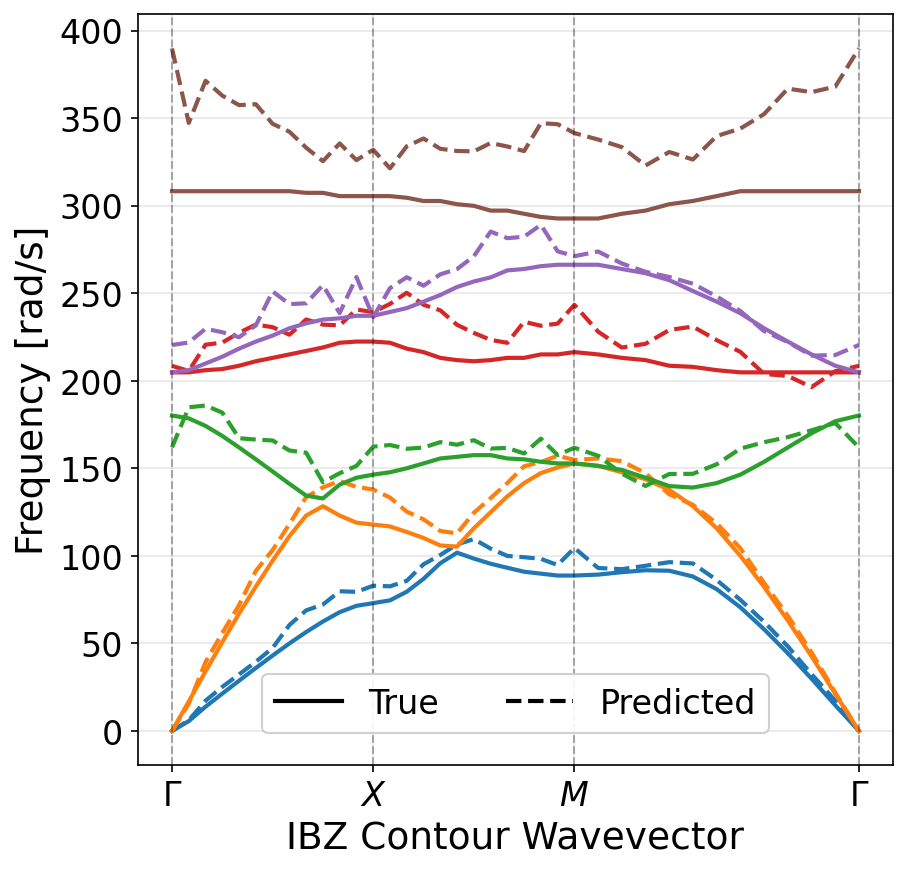
\includegraphics[width=\textwidth]{Figures/Dispersion B/NMAE754_NMSE754_g690.png}
        \caption{25th percentile performance.}
        \label{fig:dispersion_b_p25}
    \end{subfigure}
    \hfill
    \begin{subfigure}[t]{0.32\textwidth}
        \centering
        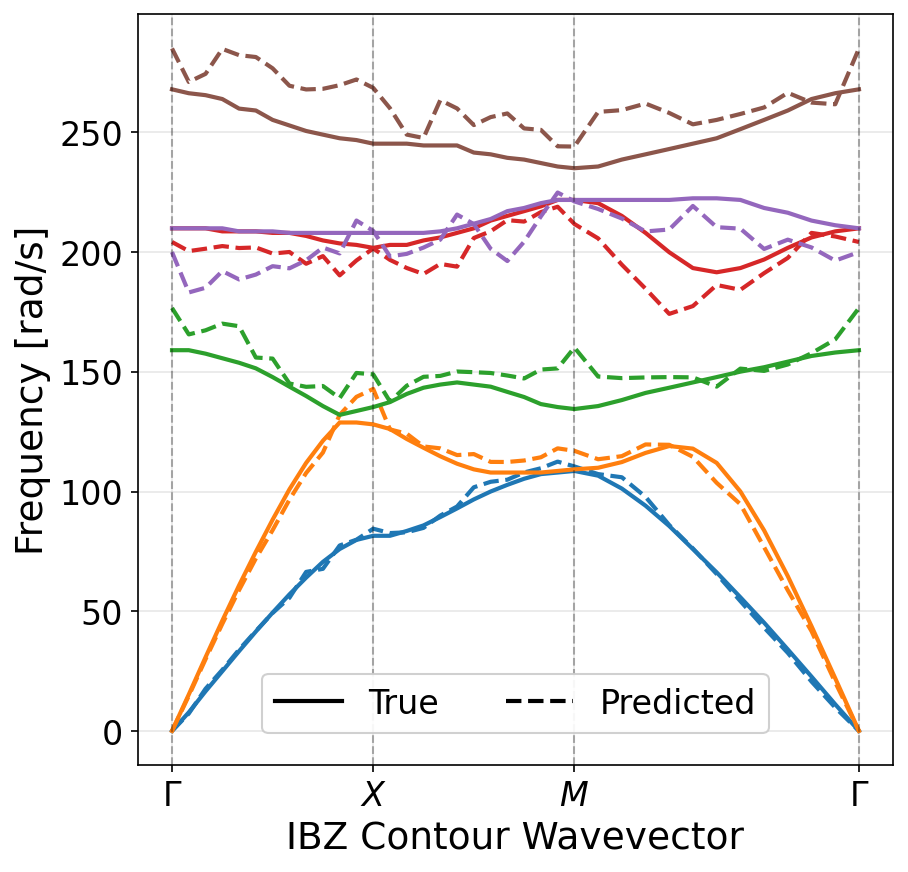
\includegraphics[width=\textwidth]{Figures/Dispersion B/NMAE499_NMSE514_g975.png}
        \caption{50th percentile performance.}
        \label{fig:dispersion_b_p50}
    \end{subfigure}
    \hfill
    \begin{subfigure}[t]{0.32\textwidth}
        \centering
        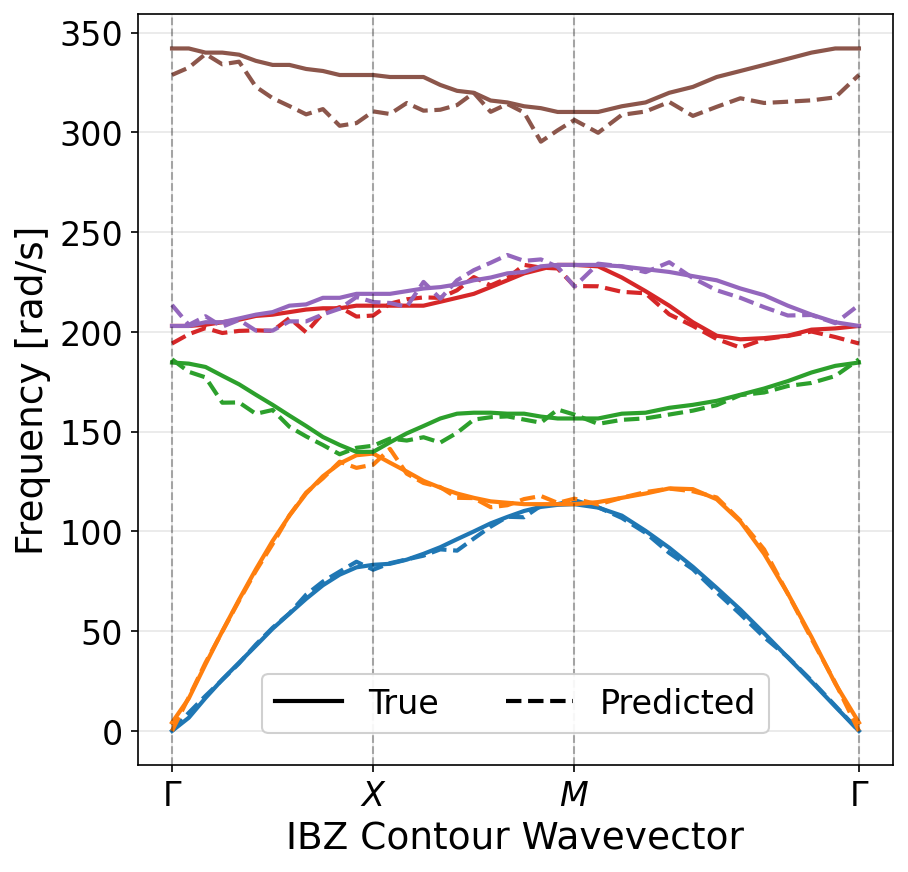
\includegraphics[width=\textwidth]{Figures/Dispersion B/NMAE252_NMSE328_g729.png}
        \caption{75th percentile performance.}
        \label{fig:dispersion_b_p75}
    \end{subfigure}
    \caption{Predicted and ground-truth dispersion bands for representative unseen discrete valued geometries spanning the 25th, 50th, and 75th percentiles of prediction performance.}
    \label{fig:dispersion_b_percentiles}
\end{figure}
Like with the continuous geometry figures, these plots represent the eigenfrequency predictions of the model across all 325 wavevectors forming the half plane for discrete valued geometries, downselected to be the horizontal, vertical, and diagonal traversal of the IBZ. Overall, the model performance is quite good at predictions in the encoded eigenfrequency, showing an average of $<1\%$ prediction error across all unseen samples.

\begin{figure}[H]
    \centering
    \begin{subfigure}[t]{0.49\textwidth}
        \centering
        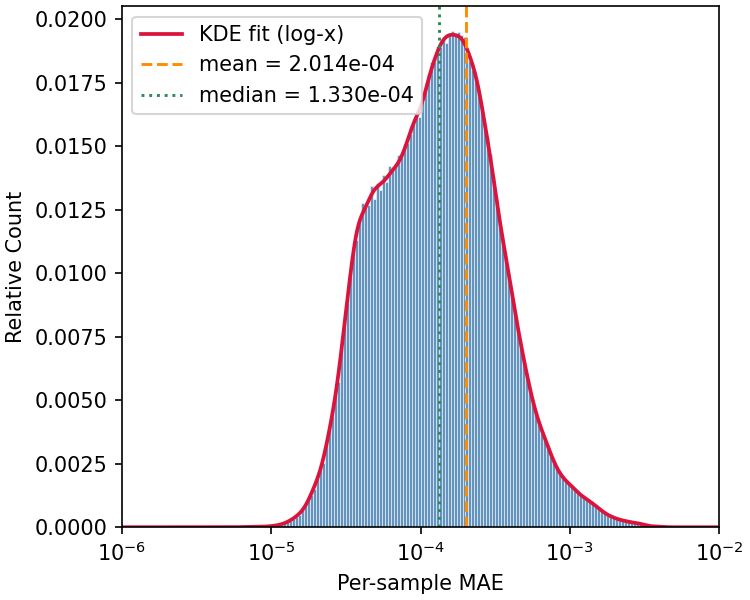
\includegraphics[width=\textwidth]{Figures/Statistics/freq_loss_histogram_mae_c_test.png}
        \caption{Performance histogram for continuous geometries.}
        \label{fig:freq_loss_histogram_continuous}
    \end{subfigure}
    \hfill
    \begin{subfigure}[t]{0.49\textwidth}
        \centering
        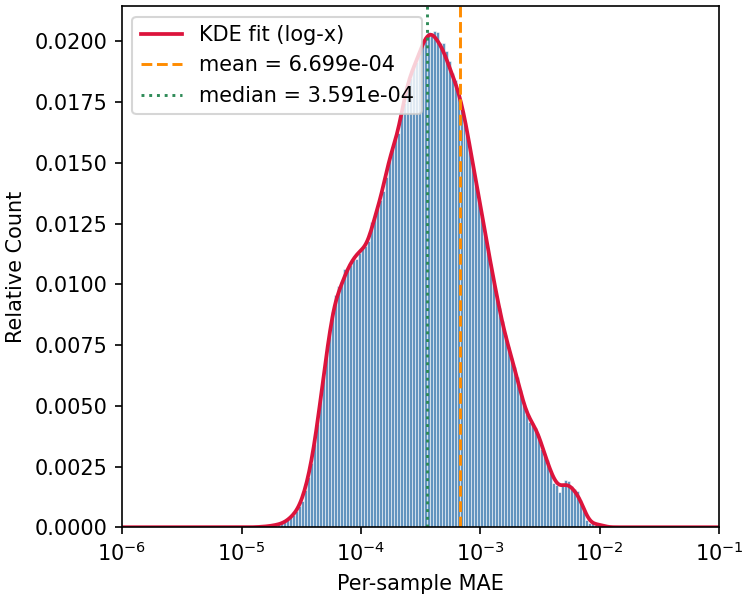
\includegraphics[width=\textwidth]{Figures/Statistics/freq_loss_histogram_mae_b_test.png}
        \caption{Performance histogram for discrete geometries.}
        \label{fig:freq_loss_histogram_discrete}
    \end{subfigure}
    \caption{Comparison of relative prediction error distributions for continuous-valued and discrete metamaterial geometries for the same model. While there are some tail outliers, most samples fall within the range of $~10^{-2}$ to $~10^{-4}$, indicating that the same model is able to learn continuous and discrete geometry cases.}
    \label{fig:freq_loss_histograms}
\end{figure}

%%%%%%%%%%%%%%%%%%%%%%%%%%%%%%%%%%%%%%%%%%%%%%%%%%%%%%%%%%%%%%%%%%%%%%
\subsection{Dependence of Prediction Error on Band and Boundary Length}
\label{ssec:boundary_length_vs_loss}

The preceding subsections showed that, although the same wavelet-conditioned FNO can predict displacement fields for both continuous and discrete unit cells, discrete geometries are systematically more difficult, with absolute and relative errors larger (Figures \ref{fig:disp_loss_histograms}, \ref{fig:freq_loss_histograms}), and the harder quartiles of the discrete test set degrading more visibly than their continuous counterparts. This gap is expected from the architecture of the FNO itself. Each Fourier layer retains only a truncated set of spectral modes after the discrete FFT. Smooth continuous material fields, and the comparatively smooth displacement modes they induce, concentrate their energy in a modest number of low-to-moderate wavenumbers and are therefore well represented by that truncated Fourier basis. Binary geometries, by contrast, contain jump discontinuities at material interfaces. Under an FFT, such discontinuities produce a broadband spectrum whose coefficients decay slowly with wavenumber, so a substantial fraction of the high-frequency content needed to resolve sharp phase boundaries lies outside the retained modes. The spectral branch therefore sees a degraded, band-limited version of the interface, yielding Gibbs-type ringing or blur and a harder operator-learning problem precisely when geometric discontinuity is more severe.
If this spectral-truncation explanation is correct, then even among discrete geometries the prediction error should increase with the boundary interface length. To test this empirically, we define the \emph{boundary length} of each binarized unit cell as the number of interior four-connected pixel edges separating a $0$-valued pixel from a $1$-valued pixel. This scalar is a discrete measure of interface complexity. For each of the $1000$ unseen discrete test geometries, we compute the mean absolute error (MAE) of the predicted displacement channels, averaged over all $325$ IBZ wavevectors, separately for each of the six retained eigenbands. The resulting relationships are shown in Figure~\ref{fig:boundary_vs_mae_by_band}.

\begin{figure}[H]
  \centering
  
\includegraphics[width=\textwidth]{Figures/Statistics/boundary_vs_mae_by_band_b_test.png}
  \caption{Mean displacement MAE versus interface boundary length, separated by color for each of the six eigenbands on the discrete test set. Points correspond to average performance on unit-cell geometries. Legend values $\rho$ are Spearman rank correlations. A positive trend appears for every band, consistent with degraded FNO accuracy as the total length of $0$/$1$ material interfaces increases.}
  \label{fig:boundary_vs_mae_by_band}
\end{figure}

Two complementary trends are apparent. First, for every band there is a positive monotonic association between boundary length and MAE, with Spearman correlations ranging from $\rho=0.644$ for band~$1$ to $\rho\approx0.42$--$0.56$ for the higher bands. Geometries with short interfaces are concentrated at lower absolute error, while geometries with long, meandering phase boundaries systematically occupy the upper portion of the cloud. This supports the interpretation that the hard cases for the learned operator are those for which the truncated Fourier representation must resolve more extensive sharp material transitions on the fixed $32\times32$ grid.
Second, absolute error itself increases with band index. Averaged over the test geometries, the mean wavevector-averaged MAE rises from approximately $1.6\times10^{-3}$ for band~$1$ to approximately $3.8\times10^{-3}$ for band~$6$. Higher bands correspond to more rapidly oscillating Bloch modes that concentrate energy nearer material interfaces and therefore inherit more of the geometric difficulty encoded by boundary length. Together with the continuous-versus-discrete comparisons above, Figure~\ref{fig:boundary_vs_mae_by_band} indicates that prediction difficulty on discrete designs is organized both by band (modal complexity) and by interface measure (geometric complexity), as expected when a spectral surrogate retains only a portion of the broadband Fourier content generated by discontinuities.

%%%%%%%%%%%%%%%%%%%%%%%%%%%%%%%%%%%%%%%%%%%%%%%%%%%%%%%%%%%%%%%%%%%%%%
\subsection{Band and Wavevector Encoding}
\label{ssec:band_wavevector_encoding}
For the FNO to ingest the conditioning constants of the eigenvalue PDE in equation \ref{eqn:eig_PDE}, namely the wavevectors $k_x$, $k_y$ and the band index $b$ that selects which eigenmode to return, these scalars must be represented as matrices or tensors compatible with the existing channel wise input structure. Alternatives that inject scalars through specialized pathways would require heavy architectural alterations, which are hard to justify given that FNO theory suggests eigenvalue PDEs should be solvable with existing hyperparameter combinations. We therefore compared three strategies for encoding these constants as input fields: constant valued fields, spatial sinusoids, and the Gabor wavelet encoding described in Section \ref{ssec:input_wavelet_encoding}.

The constant field representation is the naive default: $k_x$, $k_y$, and $b$ are each broadcast to a constant $S\times S$ channel with $S = 32$. For the wavevectors, whose physical values lie in $[-\pi,\pi]$, these constants were normalized to the interval $[-1,1]$ before broadcasting. Band indices $\{1,2,3,4,5,6\}$ were likewise normalized to the range $[0.1,0.6]$. This representation fails by mode collapse, with the FNO outputting near constant fields regardless of conditioning inputs. The cause is spectral: the FFT of a constant field is zero everywhere except at the DC coefficient, so the frequency domain branch of each Fourier layer receives no information to propagate or train on past the first layer. The Fourier branch therefore cannot contribute to the prediction, leaving only the shallow spatial domain branch, which behaves like a shallow CNN and is unable to capture the complexity of the eigenvalue problem.

A spatial sinusoidal encoding restores unique and nondegenerate representations in the spectral domain and allows the FNO to learn the problem. On pixel coordinates $(x,y)\in\{0,\ldots,S-1\}$, wavevector and band were encoded as
\[
I_k(x,y)=\cos\!\left(\frac{k_x}{S}x+\frac{k_y}{S}y\right),\qquad k_x,k_y\in[-\pi,\pi].
\]
\[
I_b(x,y)=\tfrac{1}{2}\left[\cos\!\left(\frac{2\pi b x}{S}\right)+\cos\!\left(\frac{2\pi b y}{S}\right)\right],\qquad b\in\{1,2,3,4,5,6\}.
\]
However, because a sinusoid is spectrally sparse, with energy concentrated at only a few wavenumbers, the Fourier branch remains weakly utilized, and predictions exhibit a persistent grainy, under resolved structure relative to ground truth. Increasing model depth and width did not remove this graininess, indicating the bottleneck was the encoding rather than model capacity.

The Gabor wavelet encoding resolves this by design. Wavelets are constructed to trade certainty between the spatial and spectral domains: neither representation is infinitely sharp, but both remain informationally rich. As a result, the conditioning inputs populate both branches of each Fourier layer with usable structure, both branches can train and contribute, and the model yields the accurate, well resolved predictions reported above while enabling deterministic mode selection. These observations support the broader conclusion that input encodings should be matched to the spatial and spectral structure of the operator: encodings that populate only one domain underuse the FNO's Fourier branch, whereas wavelet encodings exercise both.


\section{Conclusions}
\label{sec:Conclusion}
This work demonstrates that a single Fourier Neural Operator can learn multiple eigenmodes of the elastic wave equation across both continuous and discrete metamaterial geometries, recovering the eigenvectors as complex displacement fields and the eigenvalues as eigenfrequencies. For unseen geometries of both types, displacement predictions achieve relative errors typically between $10^{-2}$ and $10^{-4}$ and dispersion reconstructions average below $1\%$ error, showing that one model can span two very different geometry distributions and output predictions of multiple orders of magnitude while allowing the user to select any eigenmode deterministically and repeatably through arbitrary choice of conditioning inputs. This capability crucially rests on how the conditioning constants are encoded. Constant field encodings collapse to a single DC coefficient in the spectral domain, preventing the Fourier branch of the FNO from propagating information and causing mode collapse. Sinusoidal encodings are able to train meaningfully but yield grainy, under resolved predictions due to spectral model sparsity. Gabor wavelet encodings, by contrast, trade decreasing certainty in the spatial and spectral representations to maintain informationally rich representations in both domains, allowing both branches of each Fourier layer to richly interact with the data, leading to superior learning speed and prediction performance.

The same spectral perspective explains the limits we observe. Prediction error grows with the interface length of discrete geometries and with band index, consistent with the truncated Fourier representation struggling to resolve the broadband content generated by sharp material interfaces and rapidly oscillating modes. Practitioners applying FNOs to interface rich problems should therefore expect accuracy to track geometric discontinuity. Even so, the trained model is lightweight, roughly 2\,GB at float16 precision, and evaluates in about 1\,ms per sample on CPU, compared with about 1\,s per sample for the corresponding MATLAB FEA solve on CPU. This makes the FNO a compelling surrogate for iterative design and analysis in metamaterials and other fields governed by eigenvalue PDEs. Future work includes generalization to other resolutions, physics informed losses, and additional conditioning parameters such as material constants, expanding the accessible problem and solution space.

\section*{AI Usage Disclosure}
Generative AI tools were used to assist with coding of experiments, translating MATLAB code to Python, and automating training pipelines. AI tools were also used for light editing of the manuscript. All scientific claims, results, and final wording were reviewed and approved by the authors.

\section*{Declaration of Competing Interest}
The authors declare that they have no known competing financial interests or personal relationships that could have appeared to influence the work reported in this paper.

\section*{CRediT authorship contribution statement}
\noindent\textbf{Han Zhang:} Conceptualization, Data curation, Formal analysis, Investigation, Methodology, Software, Validation, Visualization, Writing -- original draft, Writing -- review and editing.\\
\noindent\textbf{Alexander Ogren:} Data curation, Software.\\
\noindent\textbf{Cynthia Rudin:} Supervision, Writing -- review and editing.\\
\noindent\textbf{Johann Guilleminot:} Formal analysis, Methodology, Supervision, Writing -- review and editing.\\
\noindent\textbf{L. Catherine Brinson:} Conceptualization, Funding acquisition, Methodology, Project administration, Resources, Software, Supervision, Visualization, Writing -- review and editing.

\section*{Data availability}
\label{sec:Repository}
Python code and experiments can be found at
\url{https://github.com/trutheresy/NO-2D-Metamaterials}.

MATLAB FEA code can be found at
\url{https://github.com/aco8ogren/2D-dispersion.git}.

\section*{Acknowledgements}
This work was supported by the NSERC Postgraduate Scholarship -- Doctoral (PGSD-599307-2025) and the NSF AI for Understanding and Designing Materials Research Traineeship (DGE-2022040).

%% If you have bibdatabase file and want bibtex to generate the
%% bibitems, please use
%%
\bibliographystyle{elsarticle-num}
%\bibliographystyle{plain} 
\bibliography{references}
%%\begin{thebibliography}{00}
%% \bibitem[Author(year)]{label}
%%\end{thebibliography}

\clearpage
\appendix

\renewcommand{\thesection}{S\arabic{section}}
\renewcommand{\thesubsection}{S\arabic{section}.\arabic{subsection}}
\renewcommand{\thefigure}{S\arabic{figure}}
\renewcommand{\thetable}{S\arabic{table}}
\renewcommand{\theequation}{S\arabic{equation}}

\setcounter{figure}{0}
\setcounter{table}{0}
\setcounter{equation}{0}

\section{Supplementary Information}
\label{sec:supplement}
\subsection{Model and Training Hyperparameters}
\begin{table}[H]
    \centering
    \begin{tabular}{|c|c|c|c|c|}
        \hline
        \textbf{Hyperparameter} &
        \multicolumn{4}{c|}{\textbf{Candidate Settings}} \\ \hline
    
        \textbf{Fourier Layers} & \textit{4} & 6 & 8 & 12 \\ \hline
        \textbf{Hidden Channels} & 32 & 64 & \textit{128} & 256 \\ \hline
        \textbf{Activation Function} & ReLU & \textit{GELU} & tanh & Sigmoid \\ \hline
        \textbf{Loss Criterion} & L1 & L2 & \textit{Huber} & SSIM \\ \hline
        \textbf{Epochs} & 8 & \textit{12} & 16 & 20 \\ \hline
        \textbf{Learning Rate} & $10^{-4}$ & \textit{$10^{-3}$} & $10^{-2}$ & $10^{-1}$ \\ \hline
        \textbf{Weight Decay} & 0 & \textit{$10^{-4}$} & $10^{-3}$ & $10^{-2}$ \\ \hline
        \textbf{Gamma} & 0 & 0.01 & \textit{0.1} & 0.5 \\ \hline
        \textbf{Step Size} & 0 & 1 & \textit{4} & 10 \\ \hline
        \textbf{Batch Size} & 64 & 128 & 256 & \textit{512} \\ \hline
        \textbf{Data Precision} & F8 E4M3 & F8 E5M2 & \textit{F16} & F32 \\ \hline
    \end{tabular}
    \caption{Combinations tried in grid search for optimal model and training hyperparameters.}
    \label{tab:training_hyperparameters}
\end{table}

\subsection{Loss Criterion}
In the exploration of optimal training protocols for the FNO model, other loss functions were trialed as training criterion: mean absolute error (MAE), mean squared error (MSE), normalized MAE, normalized MSE, Huber (smooth L1), and structural similarity index (SSI). For purposes of comparison, the validation criterion was chosen to be MAE and MSE. Broadly speaking, models that performed the best in terms of MSE also performed the best in MAE. The training criterion that yielded the lowest MAE and MSE loss was the Huber loss. All criterion followed a learning rate of $2\times10^{-3}$ with a decay factor per epoch of $0.9$. The mathematical definitions for each area as follows. Losses were evaluated and aggregated across all 5 output channels. 

\begin{itemize}
    \item The mean absolute error (MAE) loss is defined as
\begin{equation*}
    \mathcal{L}_{\text{MAE}} = \frac{1}{HW} \sum_{i=0}^{H-1} \sum_{j=0}^{W-1} \sum_{c=0}^{4} \left| \hat{u}_{c}(i,j) - u_{c}(i,j) \right|
\end{equation*}

Experimentally, models trained exclusively with MAE produced predictions with sharper interfaces and better-preserved boundary features than those trained solely with MSE. This behavior is consistent with the linear penalty of MAE, which does not disproportionately penalize isolated large residuals near discontinuities. Despite the improved qualitative sharpness, MAE training converged to higher validation MAE and MSE than Huber loss, indicating that the improved preservation of fine structural features came at the expense of overall numerical accuracy. This observation also motivated the hybrid training schedule in which optimization began with MAE before transitioning to MSE, combining the edge-preserving characteristics of MAE with the stronger refinement of large residuals provided by MSE.

\item The mean squared error (MSE) loss is defined as
\begin{equation*}
    \mathcal{L}_{\text{MSE}} = \frac{1}{HW} \sum_{i=0}^{H-1} \sum_{j=0}^{W-1} \sum_{c=0}^{4} \left( \hat{u}_{c}(i,j) - u_{c}(i,j) \right)^2
\end{equation*}

The quadratic penalty of MSE assigns increasingly large gradients to larger residuals, causing the optimizer to preferentially reduce regions with the greatest numerical error. As a consequence, the loss favors smooth predictions that minimize the overall energy of the residual rather than preserving sharp transitions. Experimentally, models trained exclusively with MSE produced outputs that reproduced the correct magnitude and large-scale structure of the solution, but exhibited diffuse interfaces and blurred boundaries. Fine-scale features were often replaced by low-amplitude, grainy artifacts, consistent with the tendency of MSE to average over uncertain or discontinuous regions in order to minimize the global squared error.

\item A hybrid MAE--MSE training schedule was also evaluated, where the model was optimized using MAE for the first half of the training epochs before switching to MSE for the remaining half. This training strategy approximates the behavior of the Huber loss over the course of optimization. During the early stages of training, prediction errors are typically large, making the linear penalty of MAE advantageous for preserving sharp interfaces while preventing large residuals from dominating the optimization. As training progresses and the average residual decreases, switching to MSE increases the emphasis on refining the remaining prediction errors and improving overall numerical accuracy.

Experimentally, this training schedule consistently outperformed training with either MAE or MSE alone for the same total number of epochs. The resulting predictions retained substantially sharper boundaries than models trained exclusively with MSE, while achieving lower validation MAE and MSE than models trained exclusively with MAE. Among the non-Huber training strategies investigated, the hybrid schedule produced the best overall balance between qualitative feature preservation and quantitative accuracy, converging to within approximately 10\% of the validation error achieved by Huber loss. Although less adaptive than Huber, which transitions between MAE- and MSE-like behavior on a per-residual basis, the epoch-wise transition captures much of the same optimization benefit.

\item The structural similarity index measure (SSIM) is defined as

\begin{equation*}
\mathcal{L}_{\text{SSIM}}
=
1
-
\frac{1}{5}
\sum_{c=0}^{4}
\frac{
\left(2\mu_{u_c}\mu_{\hat{u}_c}+C_1\right)\left(2\sigma_{u_c\hat{u}_c}+C_2\right)
}{
\left(\mu_{u_c}^2+\mu_{\hat{u}_c}^2+C_1\right)\left(\sigma_{u_c}^2+\sigma_{\hat{u}_c}^2+C_2\right)
}, \quad \text{where}
\end{equation*}
\begin{equation*}
\mu_{u_c}=\frac{1}{HW}\sum_{i=0}^{H-1}\sum_{j=0}^{W-1}u_c(i,j), \quad
\sigma_{u_c\hat{u}_c}=\frac{1}{HW}\sum_{i=0}^{H-1}\sum_{j=0}^{W-1}\left(u_c(i,j)-\mu_{u_c}\right)\left(\hat{u}_c(i,j)-\mu_{\hat{u}_c}\right)
\end{equation*}

A significant limitation of SSIM arises when it is applied to signed-valued fields. Unlike its original application to nonnegative image intensities, a perfect sign-reversed field ($\hat{u}=-u$) can achieve nearly the same SSIM score as a perfect reconstruction ($\hat{u}=u$). Consequently, a model trained solely with SSIM may converge to physically incorrect solutions containing polarity inversions while still minimizing the loss. The following derivation demonstrates the mathematical origin of this ambiguity.

For the purposes of the following discussion, we consider the common case where the stabilizing constants satisfy
\begin{equation*}
    C_1 \ll 2\mu_{u_c}^2,
    \qquad
    C_2 \ll 2\sigma_{u_c}^2,
\end{equation*}
allowing them to be neglected.

For a correct reconstruction,
\begin{equation*}
    u_c^{(+)} = u_c,
\end{equation*}
the SSIM score is
\begin{equation*}
\mathrm{SSIM}(u_c,u_c^{(+)})
=
\frac{\left(2\mu_{u_c}^2\right)\left(2\sigma_{u_c}^2\right)}
{\left(2\mu_{u_c}^2\right)\left(2\sigma_{u_c}^2\right)}
=1.
\end{equation*}

Now consider a sign-reversed reconstruction. The field and its mean reverse sign,
\begin{equation*}
    u_c^{(-)}=-u_c, \qquad \mu_{u_c^{(-)}}=-\mu_{u_c},
\end{equation*}
while the covariance reverses sign and the variance remains unchanged,
\begin{equation*}
    \sigma_{u_c,u_c^{(-)}}=-\sigma_{u_c,u_c}, \qquad \sigma_{u_c^{(-)}}^2=\sigma_{u_c}^2.
\end{equation*}
Substituting these relationships into the SSIM expression gives
\begin{equation*}
\mathrm{SSIM}(u_c,u_c^{(-)})
=
\frac{\left(-2\mu_{u_c}^2\right)\left(-2\sigma_{u_c}^2\right)}
{\left(2\mu_{u_c}^2\right)\left(2\sigma_{u_c}^2\right)}=1.
\end{equation*}
The numerator therefore differs from that of a correct reconstruction by two factors of $-1$, and thus, under these conditions, SSIM assigns essentially the same similarity score to a field and its sign-reversed counterpart as it does to a perfect reconstruction. This ambiguity constitutes a significant limitation when SSIM is applied to signed-valued regression problems where the polarity of the solution is physically meaningful. During training, the network frequently converged to predictions in which localized regions or the entire image were the negative of the correct solution while still achieving a favorable SSIM objective. Although the resulting fields exhibited accurate interface locations, boundary geometry, and overall morphology, the polarity inversions rendered the predictions physically incorrect. Consequently, SSIM should not be used as the sole training criterion for signed-valued fields unless it is supplemented by an additional loss that explicitly penalizes sign reversals.

\item The normalized mean absolute error (NMAE) loss is defined as
\begin{equation*}
    \mathcal{L}_{\text{NMAE}} = \frac{1}{HW} \sum_{i=0}^{H-1} \sum_{j=0}^{W-1} \sum_{c=0}^{4} \frac{\displaystyle \left| \hat{u}_{c}(i,j) - u_{c}(i,j) \right|}{\left| u_{c}(i,j) \right| + \varepsilon}
\end{equation*}
Unlike MAE, NMAE weights each prediction error by the inverse magnitude of the target value, causing the optimization to place greater emphasis on regions where the ground-truth solution is small in scale. Consequently, the loss seeks to minimize relative error rather than absolute error, preventing low-magnitude features from being dominated by high-magnitude regions during training.

Experimentally, NMAE successfully reduced the relative error in low-amplitude portions of the solution. However, this improvement came at the expense of increased overall MAE and MSE compared with training using the standard MAE loss. For the present application, the absolute magnitude of the prediction error was determined to be of greater practical importance than the relative error. As a result, the improved accuracy in low-valued regions did not outweigh the degradation in overall numerical accuracy, making NMAE a less suitable optimization criterion for the objectives of this work. However, for other applications, NMAE can be a valid and superior training criterion than standard MAE.

\item The normalized mean squared error (NMSE) loss is defined as
\begin{equation*}
    \mathcal{L}_{\text{NMSE}} = \frac{1}{HW} \sum_{i=0}^{H-1} \sum_{j=0}^{W-1} \sum_{c=0}^{4} \frac{\displaystyle \left(\hat{u}_{c}(i,j) - u_{c}(i,j) \right)^2}{\left( u_{c}(i,j) \right)^2 + \varepsilon}
\end{equation*}

Similar to NMAE, NMSE normalizes the prediction error by the magnitude of the target field, causing the optimization to prioritize relative error rather than absolute error. The quadratic penalty retains the characteristic behavior of MSE by assigning greater weight to larger residuals, while the normalization emphasizes regions where the target magnitude is small.

Experimentally, NMSE reduced the relative error in low-amplitude regions compared with standard MSE. However, this improvement was accompanied by increased overall validation MAE and MSE, performing worse than conventional MSE optimization. As with NMAE, the objective of this work was to minimize the absolute prediction error rather than the relative error. Consequently, the increased emphasis placed on low-magnitude regions did not translate into improved overall predictive performance, making NMSE less appropriate for the present application.
\end{itemize}

\subsection{Algorithms for Input Wavelet Encoding}
\label{ssec:input_wavelet_algorithms}
The band and wavevector conditioning channels used by the FNO are generated by the Gabor wavelet embeddings below, which match the implementations in the accompanying code.
\begin{algorithm}[H]
\caption{1D Gabor Wavelet Embedding from Band Index}
\label{alg:1d_gabor_embedding}
\begin{algorithmic}[1]
\STATE \textbf{INPUT:} Band index \( b \); grid size \( S \leftarrow 32 \); frequency scale \( r \leftarrow 2.0 \)
\STATE Create linspace vectors \( x, y \in [-1, 1] \) with \( S \) points
\STATE Construct meshgrid \( X, Y \leftarrow \text{meshgrid}(x, y) \)
\STATE Compute base frequency:
\[
f \leftarrow (1.0 + |b|) \cdot \frac{S}{8}
\]
\STATE Compute rotation angle:
\[
\theta \leftarrow (b \bmod 8) \cdot \frac{S}{16}
\]
\STATE Rotate coordinates:
\[
X_\theta \leftarrow X \cos \theta + Y \sin \theta, \quad
Y_\theta \leftarrow -X \sin \theta + Y \cos \theta
\]
\STATE Set Gaussian envelope widths:
\[
\sigma_x \leftarrow \sigma_y \leftarrow \frac{0.3}{r}
\]
\STATE Compute Gabor wavelet embedding:
\[
\psi_b(x, y) \leftarrow
\exp\left(-\frac{X_\theta^2}{2 \sigma_x^2} - \frac{Y_\theta^2}{2 \sigma_y^2}\right)
\cdot \cos(f \cdot X_\theta)
\]
\STATE \textbf{RETURN:} \( \psi_b \in \mathbb{R}^{S \times S} \)
\end{algorithmic}
\end{algorithm}

In Algorithm \ref{alg:1d_gabor_embedding}, the grid size \(S=32\) matches the geometry resolution used by the FNO. For this resolution the base frequency is \(f=(1+|b|)\,S/8\), so successive bands increase both carrier frequency and orientation. The modulo in \(\theta\) repeats orientation every eight bands, while \(f\) continues to increase, so embeddings remain distinguishable beyond eight bands. The constants \(r=2.0\), \(S/16\), and \(0.3\) were chosen so that the wavelets occupy most of the spatial domain and remain visually distinct across bands.

\begin{algorithm}[H]
\caption{2D Gabor Wavelet Embedding for Wavevectors}
\label{alg:2d_gabor_embedding}
\begin{algorithmic}[1]
\STATE \textbf{INPUT:} Wavevector components \( k_x, k_y \) (radians); grid size \( S \leftarrow 32 \); frequency scale \( r \leftarrow 1.0 \)
\STATE Set constants \( f_0 \leftarrow 2.20 \), \( \alpha \leftarrow 41 \), \( N_x \leftarrow 13 \), \( N_y \leftarrow 25 \)
\STATE Create linspace vectors \( x, y \in [-1, 1] \) with \( S \) points
\STATE Construct meshgrid \( X, Y \leftarrow \text{meshgrid}(x, y) \)
\STATE Compute frequencies:
\[
f_x \leftarrow (f_0 + k_x)\,\alpha, \quad f_y \leftarrow (f_0 + k_y)\,\alpha
\]
\STATE Compute rotation angles:
\[
\theta_x \leftarrow (k_x \bmod N_x) \cdot \frac{\pi}{N_x}, \quad \theta_y \leftarrow (k_y \bmod N_y) \cdot \frac{\pi}{N_y}
\]
\STATE Rotate coordinates:
\[
X_\theta \leftarrow X \cos \theta_x + Y \sin \theta_y, \quad
Y_\theta \leftarrow -X \sin \theta_x + Y \cos \theta_y
\]
\STATE Set Gaussian envelope widths:
\[
\sigma_x \leftarrow \sigma_y \leftarrow \frac{0.5}{r}
\]
\STATE Compute Gabor wavelet embedding:
\[
\psi_{k_x, k_y}(x, y) \leftarrow
\exp\left(-\frac{X_\theta^2}{2 \sigma_x^2} - \frac{Y_\theta^2}{2 \sigma_y^2}\right)
\cdot \sin(f_x X_\theta) \cdot \sin(f_y Y_\theta)
\]
\STATE \textbf{RETURN:} \( \psi_{k_x, k_y} \in \mathbb{R}^{S \times S} \)
\end{algorithmic}
\end{algorithm}

In Algorithm \ref{alg:2d_gabor_embedding}, \(k_x\) and \(k_y\) enter as continuous radian valued wavevector components. Distinct modulo periods \(N_x=13\) and \(N_y=25\) reduce aliasing under interchange of the two components. The offset \(f_0\) and scale \(\alpha\) map the physical range of \(k\) into carrier frequencies that remain well resolved on the \(S\times S\) grid, while \(\sigma=0.5/r\) sets the envelope width so that the patterns remain spatially localized yet informative in both domains.

\subsection{Wavelet Decoding}
\label{ssec:wavelet_decoding}
For purposes of checking general applicability, an experiment was run to check if a positive scalar may be embedded in a Gabor wavelet image and recovered after pixelization, storage, or inference. Algorithms \ref{alg:eigenfrequency_wavelet_encoding} and \ref{alg:eigenfrequency_wavelet_decoding} implement this encode--decode pair by spectral peak detection with centroid refinement. In the experiment, we test recovery over \([1,8000]\), spanning about four orders of magnitude. Despite discretization onto a finite \(S\times S\) grid and limited numeric precision associated with float16 storage and arithmetic, the decoded values remain accurate across the full range. Figures \ref{fig:eigenfrequency_encoding} and \ref{fig:eigenfrequency_decode_error} show representative encodings and the corresponding round trip error.

\begin{figure}[H]
  \centering
  
\includegraphics[width=\textwidth]{Figures/Methods/eigenfrequency_encoding.png}
  \caption{Log spaced Gabor wavelet encodings of scalars from 1 to 8000. Alternating rows show the spatial wavelet images and the corresponding Fourier magnitude spectra.}
  \label{fig:eigenfrequency_encoding}
\end{figure}

\begin{figure}[H]
  \centering
  
\includegraphics[width=\textwidth]{Figures/Methods/eigenvalue_encode_decode_error_test.png}
  \caption{Encode--decode error for scalars from a minimum of 1 to a maximum of 8000.}
  \label{fig:eigenfrequency_decode_error}
\end{figure}

\begin{algorithm}[H]
\caption{Scalar Wavelet Encoding}
\label{alg:eigenfrequency_wavelet_encoding}
\begin{algorithmic}[1]
\STATE \textbf{INPUT:} Scalar \( s>0 \); image size \( S \leftarrow 32 \); bounds \( [s_{\min}, s_{\max}] \); spectral-index bounds \( [k_{\min}, k_{\max}] \)
\STATE Set constants \( \gamma \leftarrow 1,\ \phi \leftarrow 0,\ \sigma \leftarrow 8,\ \theta_{\min}\leftarrow \pi/30,\ \theta_{\max}\leftarrow \pi/2-\pi/30 \)
\STATE Compute log-domain values:
\[
\ell_s \leftarrow \log s,\quad \ell_{\min}\leftarrow \log s_{\min},\quad \ell_{\max}\leftarrow \log s_{\max}
\]
\STATE Compute normalized position and spectral index:
\[
t \leftarrow \mathrm{clip}\!\left(\frac{\ell_s-\ell_{\min}}{\ell_{\max}-\ell_{\min}},0,1\right),\quad
k \leftarrow k_{\min} + t\,(k_{\max}-k_{\min})
\]
\STATE Compute log width per unit \(k\):
\[
\Delta_\ell \leftarrow \frac{\ell_{\max}-\ell_{\min}}{k_{\max}-k_{\min}}
\]
\STATE Compute orientation from within-band log position:
\[
\theta \leftarrow \theta_{\min} + \left(\frac{(\ell_s-\ell_{\min})\bmod \Delta_\ell}{\Delta_\ell}\right)\left(\theta_{\max}-\theta_{\min}\right)
\]
\STATE Build centered grid \(X,Y \in \{-S/2,\dots,S/2-1\}\), then rotate:
\[
X_\theta \leftarrow X\cos\theta + Y\sin\theta,\quad
Y_\theta \leftarrow -X\sin\theta + Y\cos\theta
\]
\STATE Set envelope widths \( \sigma_x \leftarrow \sigma,\ \sigma_y \leftarrow \gamma \sigma_x \), and carrier frequency \( \omega \leftarrow 2\pi k/S \)
\STATE Compute wavelet image:
\[
\psi_s \leftarrow
\exp\!\left(-\frac{1}{2}\left(\frac{X_\theta^2}{\sigma_x^2}+\frac{Y_\theta^2}{\sigma_y^2}\right)\right)\cos(\omega X_\theta+\phi)
\]
\STATE \textbf{RETURN:} \( \psi_s \in \mathbb{R}^{S\times S},\ k,\ \theta \)
\end{algorithmic}
\end{algorithm}

\begin{algorithm}[H]
\caption{Scalar Wavelet Decoding}
\label{alg:eigenfrequency_wavelet_decoding}
\begin{algorithmic}[1]
\STATE \textbf{INPUT:} Wavelet image \( \psi \in \mathbb{R}^{S\times S} \); bounds \( [s_{\min}, s_{\max}] \), \( [k_{\min}, k_{\max}] \), \( [\theta_{\min}, \theta_{\max}] \)
\STATE Set constants for centroid refinement: radius \(R\leftarrow 3\), power \(p\leftarrow 2\)
\STATE Mean-center image \( \psi_c \leftarrow \psi - \mathrm{mean}(\psi) \), then compute the centered 2D discrete Fourier magnitude:
\[
\hat{\psi}(k_x,k_y)\leftarrow \sum_{m=0}^{S-1}\sum_{n=0}^{S-1}\psi_c(m,n)\,
\exp\!\left(-2\pi i\!\left(\frac{k_x m}{S}+\frac{k_y n}{S}\right)\right),\quad
F(k_x,k_y)\leftarrow |\hat{\psi}(k_x,k_y)|
\]
\STATE Keep upper-half-plane spectral support (plus positive-frequency center row) and find dominant peak index \( (r^{*},c^{*}) \)
\STATE Define symmetric peak partner about center, then compute weighted local centroid around \( (r^{*},c^{*}) \) within radius \(R\), using weights \(w=F^p\) and excluding points closer to the symmetric partner
\STATE Convert refined centroid to wavevector coordinates \( (k_x,k_y) \), then:
\[
k_{\mathrm{ext}} \leftarrow \sqrt{k_x^2+k_y^2},\quad
\theta_{\mathrm{ext}} \leftarrow \operatorname{atan2}(k_y,k_x)\bmod \pi
\]
\STATE Map extracted \(k\) to approximate log value:
\[
\ell_{\mathrm{approx}} \leftarrow \ell_{\min} + \mathrm{clip}\!\left(\frac{k_{\mathrm{ext}}-k_{\min}}{k_{\max}-k_{\min}},0,1\right)\,(\ell_{\max}-\ell_{\min})
\]
\STATE Let \( \Delta_\ell \leftarrow (\ell_{\max}-\ell_{\min})/(k_{\max}-k_{\min}) \), compute within-band position from angle:
\[
\alpha \leftarrow \mathrm{clip}\!\left(\frac{\theta_{\mathrm{ext}}-\theta_{\min}}{\theta_{\max}-\theta_{\min}},0,1\right),\quad
\delta_\ell \leftarrow \alpha\,\Delta_\ell
\]
\STATE Find nearest consistent log value by testing neighboring bands \(b-1,b,b+1\):
\[
\ell^\star \leftarrow \arg\min_{\ell \in \{\ell_{\min} + j\Delta_\ell + \delta_\ell\}} |\ell-\ell_{\mathrm{approx}}|
\]
\STATE Clip \( \ell^\star \) to \( [\ell_{\min},\ell_{\max}] \), then decode:
\[
s_{\mathrm{ext}} \leftarrow \exp(\ell^\star)
\]
\STATE \textbf{RETURN:} \( s_{\mathrm{ext}},\ k_{\mathrm{ext}},\ \theta_{\mathrm{ext}} \)
\end{algorithmic}
\end{algorithm}

Algorithms \ref{alg:eigenfrequency_wavelet_encoding} and \ref{alg:eigenfrequency_wavelet_decoding} summarize the forward and inverse mapping used in this experiment. The forward mapping places the scalar on a log scale and jointly encodes magnitude and orientation into a Gabor-like pattern. The inverse mapping recovers an estimate by spectral peak detection with centroid refinement, followed by a consistency step that combines extracted magnitude and angle to reconstruct the most likely log value.

\end{document}

\endinput
%%
%% End of file `elsarticle-template-harv.tex'.
